\documentclass[openany, 11pt]{book}

\usepackage{titlesec}
\usepackage{geometry}
\usepackage{chngcntr}
\usepackage{tabularx}
\usepackage{hyperref} % Add the hyperref package for clickable links
\usepackage{parskip}
\usepackage{enumitem}
\usepackage{amsmath}
\usepackage{graphicx}
\usepackage{amssymb}
\usepackage{soul}
\usepackage{tcolorbox}
\usepackage{ulem}
\usepackage[absolute,overlay]{textpos}
\usepackage{xcolor}
\usepackage{booktabs}
\usepackage{pdflscape}
\usepackage{fancyhdr}
\usepackage{wasysym}
\usepackage{textcomp}
\usepackage{wrapfig}

\tcbuselibrary{skins}

\geometry{a4paper, margin=1in} % Adjust margins as needed

% Define chapter title format
\titleformat{\chapter}[display]
{\normalfont\bfseries\centering}{\vspace*{-2cm}}{0pt}{\LARGE}

% Redefine \thesection to suppress chapter number in TOC
\renewcommand{\thesection}{\arabic{section}}

% Adjust spacing around chapter titles
\titlespacing{\chapter}{0pt}{12pt}{6pt}

% Adjust spacing around section headers
\titlespacing{\section}{0pt}{8pt}{2pt}

% Configure hyperref to make only the first-level entries clickable
\hypersetup{
    linktoc=page,
    linktocpage=true
}

\setlist{topsep=0pt, partopsep=0pt, parsep=0pt, itemsep=0pt}

\newtcolorbox{notebox}{
    colback=blue!5!white,
    colframe=blue!75!black,
    fonttitle=\bfseries,
    title=Note
}

% Clear default header/footer settings
\fancyhf{}

% Set page number on the left for even pages and the right for odd pages
\fancyfoot[LE,RO]{\thepage}

% Set line at the top of the page
\renewcommand{\headrulewidth}{0pt}

% Apply the settings
\pagestyle{fancy}

% \cover command
%
% This command creates a cover block with a specified size and text color.
%
% Parameters:
% #1 (optional): Text color (default: white)
% #2: X-coordinate of the top-left corner of the block, in pt
% #3: Y-coordinate of the top-left corner of the block, in pt
% #4: Width of the block, in cm
% #5: Height of the block, in cm
%
% Usage:
% \cover{1}{2}{3}{4} % Default text color (white)
% \cover[black]{5}{6}{2}{2} % Specified text color (black)
%
% Notes:
% - If the optional text color argument is not provided, the default is white.
%
% Example:
% \cover[red]{10}{20}{3}{3} % Creates a red cover block at coordinates (10pt, 20pt) with a size of 3x3 cm.
\newcommand{\cover}[5][white]{%
    \begin{textblock*}{3cm}(#2pt,#3pt)
        \colorbox{white}{\textcolor{#1}{\rule{#4cm}{#5cm}}}
    \end{textblock*}%
}

\begin{document}

    \title{Universal Milling Machine SCHAUBLIN 13 Manual}
    \author{}
    \date{}
    \maketitle

    \tableofcontents

    \chapter{Principal Technical Data}

\section*{Table}
\begin{tabularx}{\textwidth}{lX}
    Useful area        & 600 x 210 mm \\
    Number of T-slots  & 4            \\
    Width of T-slots   & 12 mm        \\
    Spacing of T-slots & 40 mm        \\
\end{tabularx}

\section*{Table Movements}
\begin{tabular}{ll}
    Longitudinal (by means of feed-spindle or lever) & 260 mm  \\
    Longitudinal (with crosspiece)                   & 310 mm  \\
    Vertical (by feed-spindle only)                  & 310 mm. \\
\end{tabular}

\section*{Automatic Table Movement}
\begin{tabular}{ll}
    8 longitudinal feeds & 11 to 210 mm/min. \\
    8 vertical feeds     & 11 to 210 mm/min. \\
\end{tabular}

\section*{High Speed Table Feed}
(Only if specially ordered)
\begin{tabular}{ll}
    Longitudinal and vertical & 1000 mm/min. \\
\end{tabular}

\section*{Spindle Head}
\begin{tabular}{ll}
    Axial Stroke (By feed spindle or lever)   & 150 mm.             \\
    Internal Taper                            & ISO 30              \\
    Spindle Bore                              & Ø 15 mm             \\
    Diameter of cutter arbors, long and short & 13-16-22-25,4-27 mm
\end{tabular}

\section*{Spindle Speeds}
\begin{tabular}{ll}
(by infinitely-variable gear)
    & 58 - 2000 rpm \\
\end{tabular}

\section*{Spindle Drive Motor}
\begin{tabular}{ll}
    Power & 2 HP        \\
    Speed & 1500 r.p.m. \\
\end{tabular}

\section*{Dimensions}
\begin{tabular}{ll}
    Weight                                & 500 kg (1100 lbs.) \\
    Space required; length, depth, height & 124 x 80 x 150 cm  \\
\end{tabular}

    \newpage
\begin{figure}[h]
    \centering
    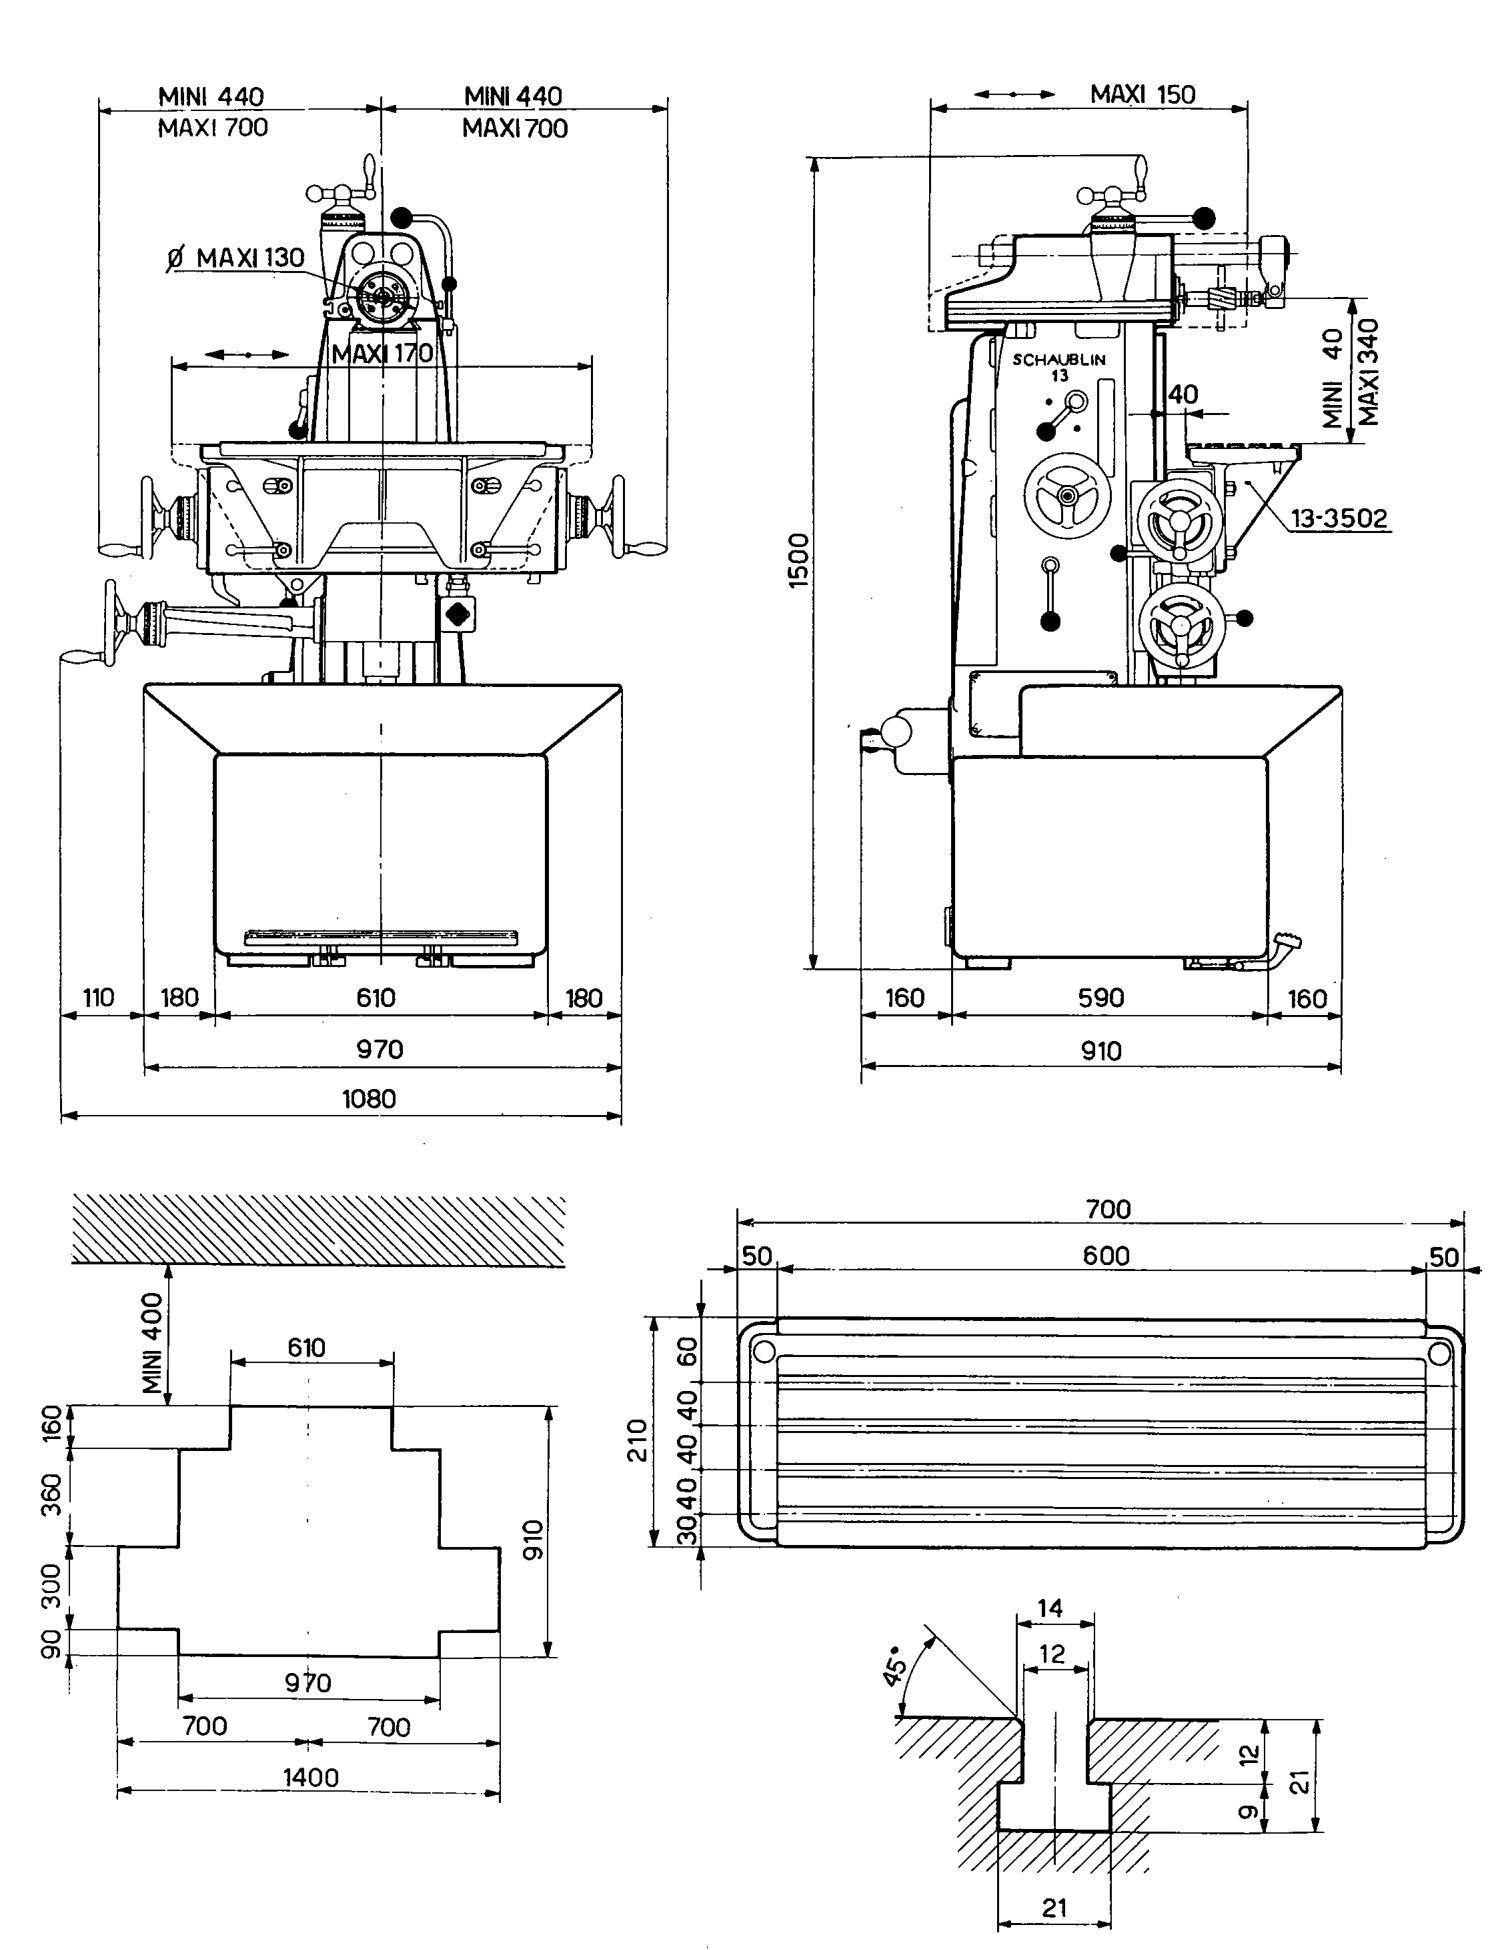
\includegraphics[width=1.0\linewidth]{images/page_7}
    \label{fig:main_dimensions}
\end{figure}

    \chapter{Erection}

\section*{Handling}
On receipt of the machine, uns crew the top of case and remove
sides, unscrew the four fixing bolts and take out the machine.
Take care to recover any accessories which may be included among
the packing.
The machine weighs approximately 500 kilos (1100 lbs.). When
handling the machine with the aid of hoisting tackle, it should
be slung as shown in the drawing on page 8. The hook should be
wrapped with rags and the table is locked in its bottom position
(without the swarf tray).

\section*{Concrete Foundation}
The Schaublin 13 Miller is designed for erection on a concrete
foundation, the dimensions of the latter being as shown in the
foundation drawing on page 8. The depth of the foundation will
depend on the nature of the ground; the concreting should be done
on firm ground only.
The electric supply leads can be laid either above ground,
through the gap between the floor and the frame, or underground
along a channel leading to point 4. In this latter case it is
advisable to provide in the concrete foundation a steel pipe 2
with an inside diameter of 26 mm., 155 mm. long. The electric
supply cable must project about 24" above the floor.
The machine is secured to the concrete foundation by means of
4 stay-bolts 1, these latter being first inserted in the holes
provided in the concrete. With the aid of 4 flat steel strips 3,
placed under the feet of the machine, the latter is levelled
and vertically trued by means of a precision spirit-level.
When this has been done, the staybolts, iron strips and machine
feet are grouted in with cement, care being taken to keep the
machine correctly levelled and trued.
The holes provided in the machine base to accommodate the fixing
bolts are 14 mm. in diameter. The stay-bolts, nuts and strips
for fixing the machine are not supplied with the latter.
The machine must be accessible from every direction. (see page 6). % TODO: add page reference

\section*{Cleaning}
Only clean, chemically neutral and preferably white rags should
be used for degreasing and cleaning.
First remove the anti-rust grease with a dry scouring cloth,
and then wipe the surfaces over with a rag dipped in paraffin
and wrung out. The anti-rust grease has no lubricating proper-
ties whatever, and must be completely removed as its presence
may cause serious seizing, often weeks after the machine has
been started up. Care should be taken during cleaning operations
to ensure that no scratches are produced, especially on the
saddle and milling-spindle head guides.
Finally, all bright surfaces should be coated with a light film
of lubricating oil.

    \newpage
\begin{figure}[h]
    \centering
    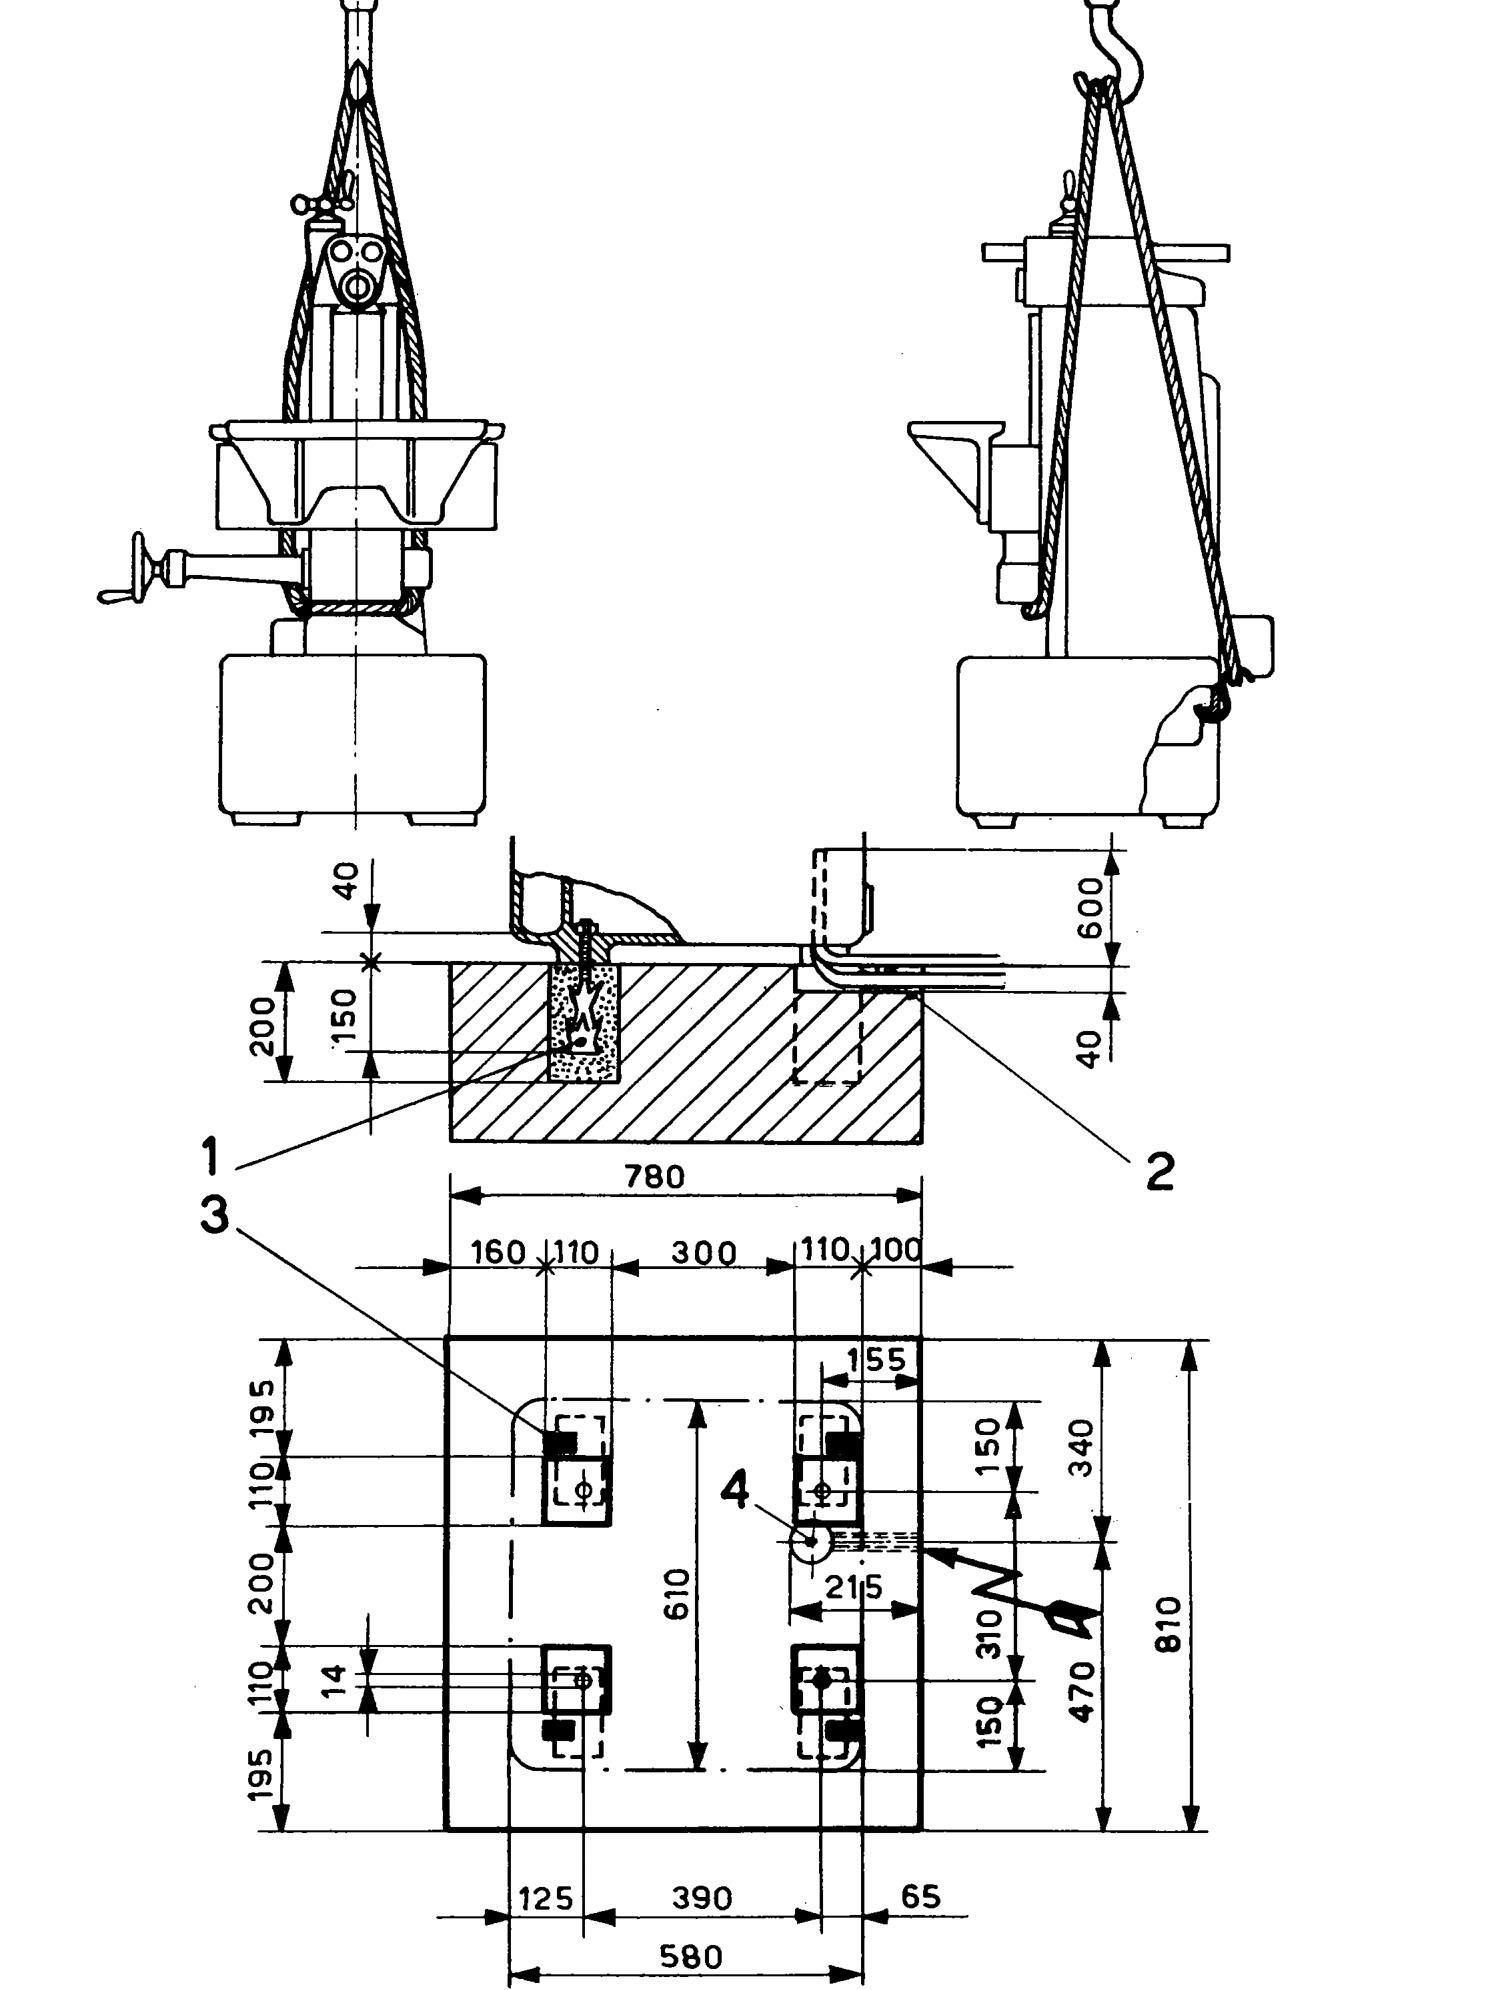
\includegraphics[width=1.0\linewidth]{images/page_9}
    \label{fig:transport_and_floorplan}
\end{figure}

    \chapter{Lubrication and Maintenance}

Before the Miller is started up, all its operative parts must be
thoroughly oiled. We recommend for this purpose an oil having the
following characteristics:-

\begin{center}
    VISCOSITY 4,5°E at 50°C
\end{center}

The viscosity of the oil in the two oil baths must not exceed
4,5°E at 50°C. The following is the correct procedure for filling
the oil baths: -

\section*{Gearbox Oil Bath}

Slacken screw 5 and remove clamping-piece 6. Pull one of the
surrpoting arms 7 rearwards until the passage between the arm
guide hole and the clamping hole is clear. Fill, through the
apertune thus provided, up to the mark on the oil level gauge 8.
Drain by removing screw 9. (See page 10, A, and page 21).

\section*{Feed box Oil Bath}

Unscrew oil-level indicator 10 and fill up until the gears dip
into the oil (test by turning the wheels). A quantity of 0,2
litre (about 1/3 pint) is sufficient. Drain by unscrewing screw
11. (See page 10, B).

\section*{Draining the oil baths}

Once a year, drain the two oil baths, swill them out with
paraffin, and refill.

\section*{Lubricating the Variator}

Remove the cover 12 and fill the small reservoir with oil.
Check oil level weekly.

\section*{Lubricating the motors}

The bearings of the main drive motor, the high-speed feed motor
and the coolant pump motor should be greased with ball-bearing
grease. The instructions enclosed herewith contain full particulars
as to maintenance and lubrication of the motors.

\section*{Pressure Lubrication}

The other parts of the machine are lubricated once a week by
injection oil with an oil gun. All lubricating points are
indicated on page 11. 4 to 5 shots of oil per nipple are
sufficient.

\underline{The feed box is to be lubricated 2 - 3 times a week through red oil nipple.}

\section*{Lubricating the Vertical Feed Spindle}

Raise the table to its top position. Lift the telescoping guard
tubes and oil the feed-spindle with a hand oilcan. This operation
should be performed once weekly.

    \newpage
\begin{figure}[h]
    \centering
    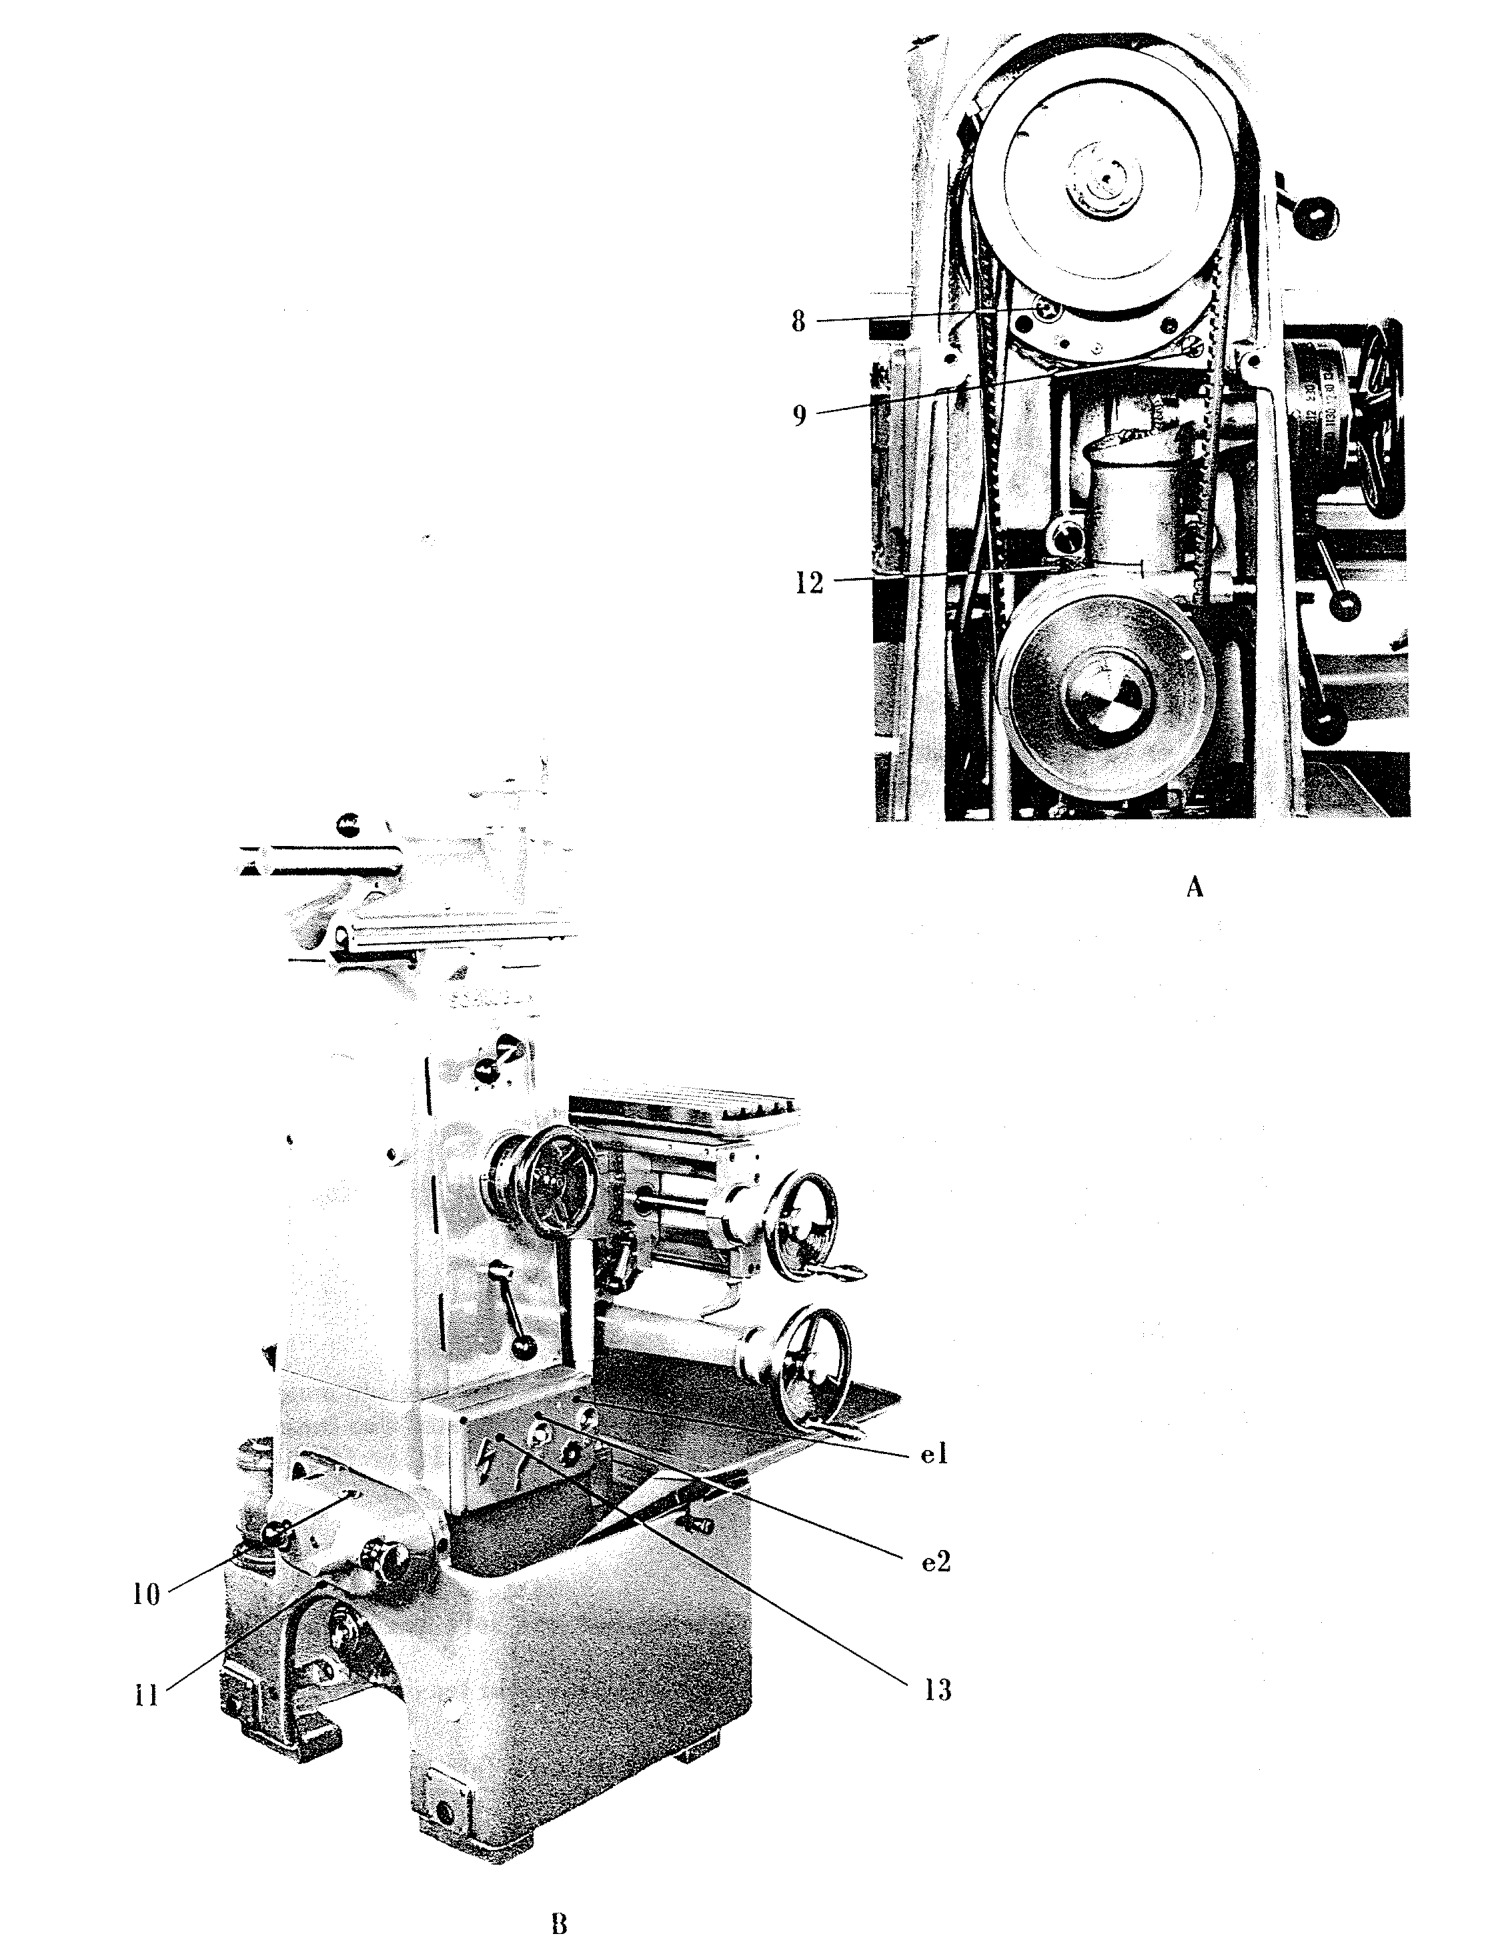
\includegraphics[width=1.0\linewidth]{images/page_11}
    \label{fig:oil_and_electronics}
\end{figure}

    \newpage
\begin{figure}[h]
    \centering
    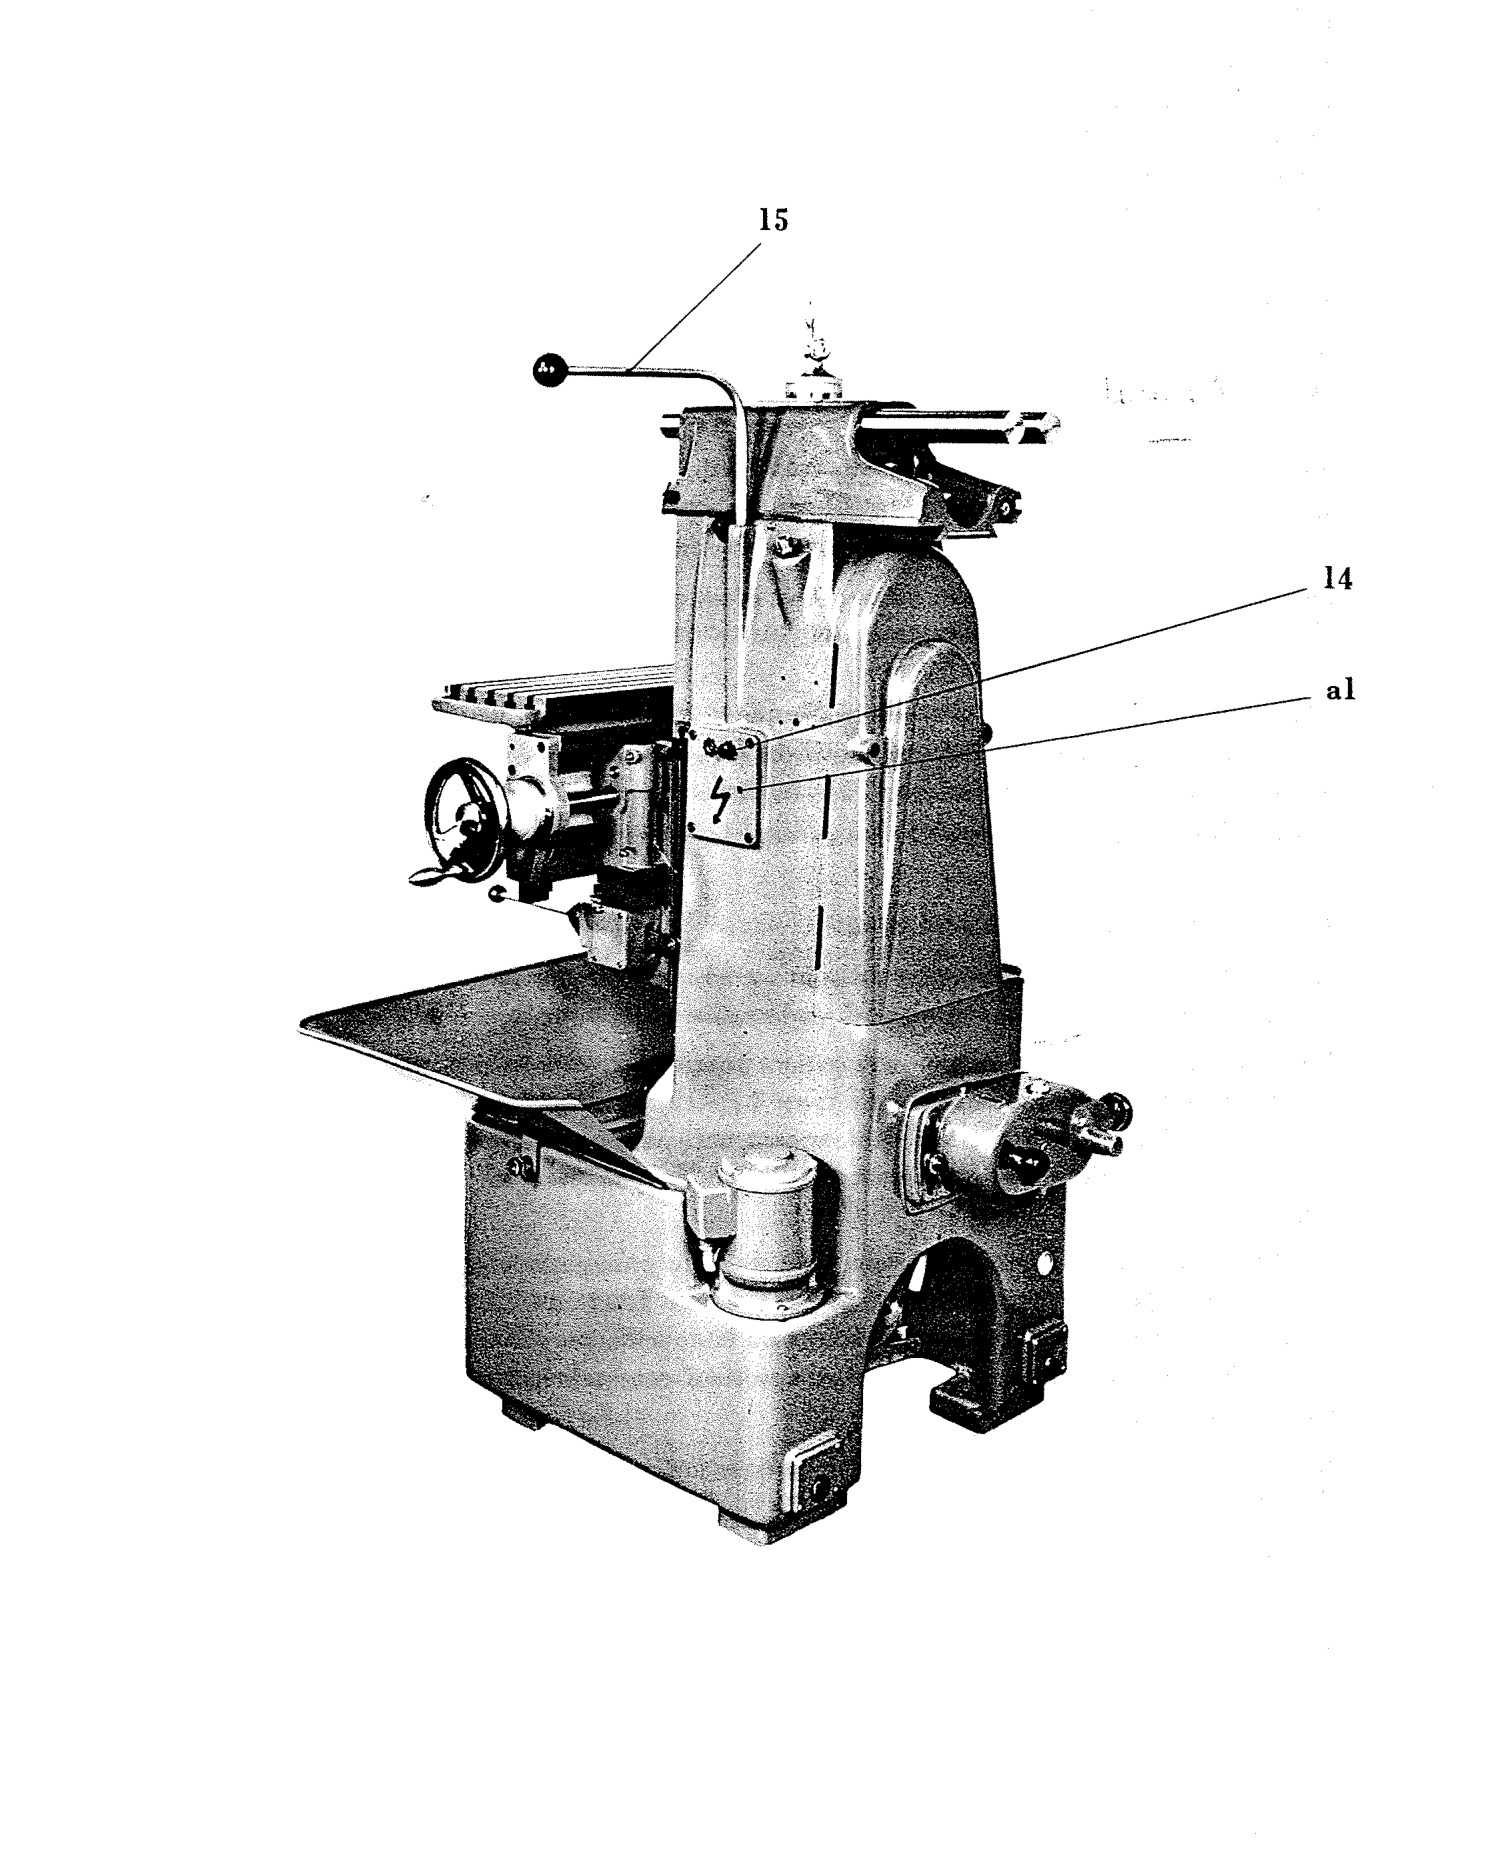
\includegraphics[width=1.0\linewidth]{images/page_12}
    \label{fig:spindle_controls}
\end{figure}

    \chapter{Electrical Equipment}

The Schaublin 13 Universal Miller is always delivered with complete
electrical equipment (motors, switches, motor protection switches
and wiring) ready for connecting to the mains. Before connecting
the machine up to the mains, make sure that the voltage specified
on the machine data plate tallies with that of the mains supply.
For wiring diagram, see page 14.

\section*{Connecting Up}

The machine is normally supplied with three-phase motors. The mains
connection terminals RST are located in the terminal box 13, this
being in the base. The machine is earthed via the yellow terminal
in the terminal box. When the current is switched on, make sure that
the motors are running in the correct direction, the procedure being
as follows:-

Place the screw 14 in the centre of that of the 2 milling cutters
outlined on the plate that corresponds to the cutter fitted to the
milling spindle, and turn the control lever 15 in the direction now
possible. The milling spindle must now rotate in the direction
indicated on the plate. (See page 11).

\section*{Description of the Equipment}

The Miller is equipped with three motors; one for the milling
spindle drive and table feeds, one for the high-speed table feed,
and one for the coolant pump.

\subsection*{Spindle and Table-feed Motor 16}

Type Oerlikon N84-2-4, three-phase, short-circuited rotor, power
2 HP, speed 1410 r.p.m. Connection box on right as viewed from end
of shaft.

\subsection*{High-speed Feed Motor 17}

Type Schindler KDWF03, power 0,3 HP, speed 2800 r.p.m. 3 x 3 mm.
key on end of shaft.

\subsection*{Coolant Pump Motor 18}

Vertical type, power 0,1 HP, speed 2800 r.p.m.
The spindle and pump motors are controlled and protected by the
"CHC" switching contactors 19, type VTp 15, mounted in the machine
frame. In the event of the motors being overloaded for a protracted
period, these contactors automatically switch off. The motors are
restarted by pressing push-buttons 20 ans 21 (See page 17).

Switch 22 is used for switching on and reversing the milling
spindle motor, lever 15 being moved to left or right according
to the position of screw 14.

Switch 23 enables the high-speed feed motor to be switched on
by means of a pedal 24 provided in front of the base.

This motor is protected from overloading by a friction clutch.

The coolant pump motor is switched on by means of the push-
button 21 of the contactor located underneath the plate showing
a cock.

Directions concerning the motors are attached to these present
instructions.

\section*{Starting Up}

When all instructions regarding erection, cleaning, lubrication
and electrical equipment have been carried out, start the machine
up and let it run idle for several hours. Start with a low speed.
to enable the bearings and transmission members to warm up
normally, then gradually increase to maximum speed. Check the
proper functioning of each part.

    \chapter{List of Devices}

\begin{description}
    \item[al] \underline{Rotation direction switch for m1} \\
    Manufacturer: Ghielmetti \& Co. S.A., \underline{Soleure} \\
    Type: HKR N° 7141, Schema 42.008 \\
    Dimensions: 6081 III (5 poles)

    \item[a2] \underline{Push-button switch for $m_3$} \\
    Manufacturer: Ghielmetti \& Co. S.A., \underline{Soleure} \\
    Type: Dr A, 3 poles, Schema S 46465 - Nr. 71.203 \\
    Dimensions: 5371/3. According to sketch 664.

    \item[el] \underline{Protection switch for $m_1$} \\
    Manufacturer: Carl Meier \& Co., \underline{Schaffhouse} \\
    Type: VTp 15, fig. 73404 \\
    \begin{tabular}{@{}ll}
        Adjustable thermal settings: & $6.4 - 10\,\mathrm{A}$ for $220\mathrm{V}$   \\
        & $4.8 - 7.5\,\mathrm{A}$ for $250\mathrm{V}$  \\
        & $3.2 - 5\,\mathrm{A}$ for $380\mathrm{V}$    \\
        & $2.4 - 3.75\,\mathrm{A}$ for $500\mathrm{V}$
    \end{tabular}

    \item[e2] \underline{Protection switch for $m_2$} \\
    Manufacturer: Carl Meier \& Co., \underline{Schaffhouse} \\
    Type: VTp 15, fig. 73404 \\
    \begin{tabular}{@{}ll}
        Adjustable thermal settings: & $0.28 - 0.5$ for $220 - 380\,\mathrm{V}$ \\
        & $0.17 - 0.3$ for $500\,\mathrm{V}$       \\
    \end{tabular}

    \item[m1] \underline{Spindle motor} \\
    Manufacturer: Atelier de construction Oerlikon, \underline{Zürich-Oerlikon} \\
    Type: 145 cz-4 three-phase with multiple and deep notched armature \\
    Power: $2\,\mathrm{HP}$ at $1410\,\mathrm{rpm}$ \\
    Sketch N° L 018002. Terminal layout on the right, viewed from the shaft end.

    \item[m2] \underline{Pump Motor} \\
    Manufacturer: Rüetschi, \underline{Suhr} \\
    Type: 70/2 - 140 \\
    Power: $0.15\,\mathrm{HP}$ \\
    Speed: $2800\,\mathrm{rpm}$

    \item[m3] \underline{Rapid feeds motor} \\
    Manufacturer: EMB Birsfelden \\
    Type EMB: $300\,\mathrm{rpm}$, $0.6\,\mathrm{HP}$ \\
    Key $3 \times 3$ on the shaft end (terminal layout and mounting holes per drawing 13-1068).
\end{description}

    \newpage

\vspace*{\fill}
\begin{center}
    Electrical diagram attached (see end of the manual)
\end{center}
\vspace*{\fill}
\label{page:electrical_diagram_attached}

    \chapter{Structural Details and Controls}\label{chap:structural_characteristics_and_handling}

\section*{Spindle Head}

The spindle head can be moved axially on the head frame by means
of a handwheel 25, with vernier, accessible from all directions.
The screw spindle has a pitch of 4 mm. The vernier is graduated
in 2/100 mm. and can be set at zero. The milling spindle 26, of
hardened chrome-nickel steel, runs in high-precision ball bearings.
The spindle nose is of the following type: ASA B5 18-1943 N° 30
(dimensions see page 21).

For adjustment of spindle bearings, see page 20.
The front of the spindle head is machined and the two supporting
arms 7 enable the special attachments and the outside bracket
for guiding the long milling-cutter arbors to be mounted.

\section*{frame}

The powerfully-ribbed frame is cast integral with the base in
extremely hard alloy cast iron, and its lower part houses the
drive members for the milling spindle and the feed gear, as well
as the coolant tank.

The upper portion of the frame encloses the gearbox, in which
all the gears are made of hardened and ground chrome-nickel
șteel. In conjunction with the speed regulator, which is likewise
mounted in the frame, this gear provides the very wide range of
speeds of 56 to 2100 r.p.m.

\section*{Starting Up}

Switch 22, housed in a case on the right-hand side of the frame,
enables the milling spindle to be started up and reversed with.
the aid of the lever 15. This lever is locked by means of screw
14, so that the direction of rotation, once set, is maintained.
If this screw is fitted in the centre of one the milling cutters
sketched on the plate - the one corresponding to the cutter
fitted to the spindle - the desired direction on rotation is
automatically obtained.

When the machine is shut down for a protracted period, it is
advisable to switch off the motor by means of the contactor
indicated by a plate bearing the image of a milling cutter.
The high-speed feed motor is started up by means of the
pedal 24 and the push-button switch 23 located respectively in
front of and on the base.

The coolant pump motor is started up by the push-button 21 on
the contactor marked by a plate showing a cock.

    \chapter{Control and Selection of the Spindle Speeds}
\section*{Spindle Speeds}

Speeds ranging from 56 to 2100 r.p.m., infinitely variable within
these limits, are obtained by means of a belt-type speed-change
gear. The drive is transmitted from the motor to the speed
regulator and the gearbox by means of 2 vee-belts answering to
the following specification:

\begin{itemize}
    \item Brand: Dayton,
    \item Profile: 1 1/\(32"\) x 11/32"
    \item Angle: \(30^\circ\)
    \item Mean length: 48"
\end{itemize}

For instructions as to adjustment of variator, see page \pageref{chap:spindle_speed_variator}.

\section*{Selection of Speeds}

The speed of the belt-type speed-change gear is varied by means
of the handwheel 28, which is locked by means of the knob 29.
The change over from low to high speed is effected by the lever 30.

Handwheel 28 must be operated with the motor running, whereas
\ul{lever 30 must be operated only when the machine is at a standstill.}

If, for instance, a spindle speed of 180 r.p.m. is desired,
handwheel 28 must be turned until the figure 180 appears opposite
the pointer 31. The colours on the spindle-speed scale tally with
the colours marking the positions of the lever 30 (for 180 r.p.m.,
green).

Lever 15, operated in conjuction with a switch, enables the
spindle to be run in either direction (see page \pageref{chap:structural_characteristics_and_handling}, "Starting up").

\section*{Vertical Slide}
\subsection*{Hand Feed}
Hand feed is controlled by means of the handwheel 32.
The vertical feed-spindle has a pitch of 4 mm. and the scale
is graduated in 2/100 mm.; it can be set at zero.

\subsection*{Locking the Vertical Slide}

The vertical slide is locked by means of lever 33.

\section*{Longitudinal Slide}
\subsection*{Hand Feed}

Longitudinal hand feed is controlled by handwheel 34.
The longitudinal spindle has a pitch of 4 mm. and the scale is
graduated in 2/100 mm.; it can be set at zero.

\subsection*{Locking the Longitudinal Slide}

The longitudinal slide is locked by means of lever 35.
ADJUSTING THE TAPER STRIPS of the vertical and longitudinal
slides and spindle head; see page 24.

    \newpage
\begin{figure}[h]
    \centering
    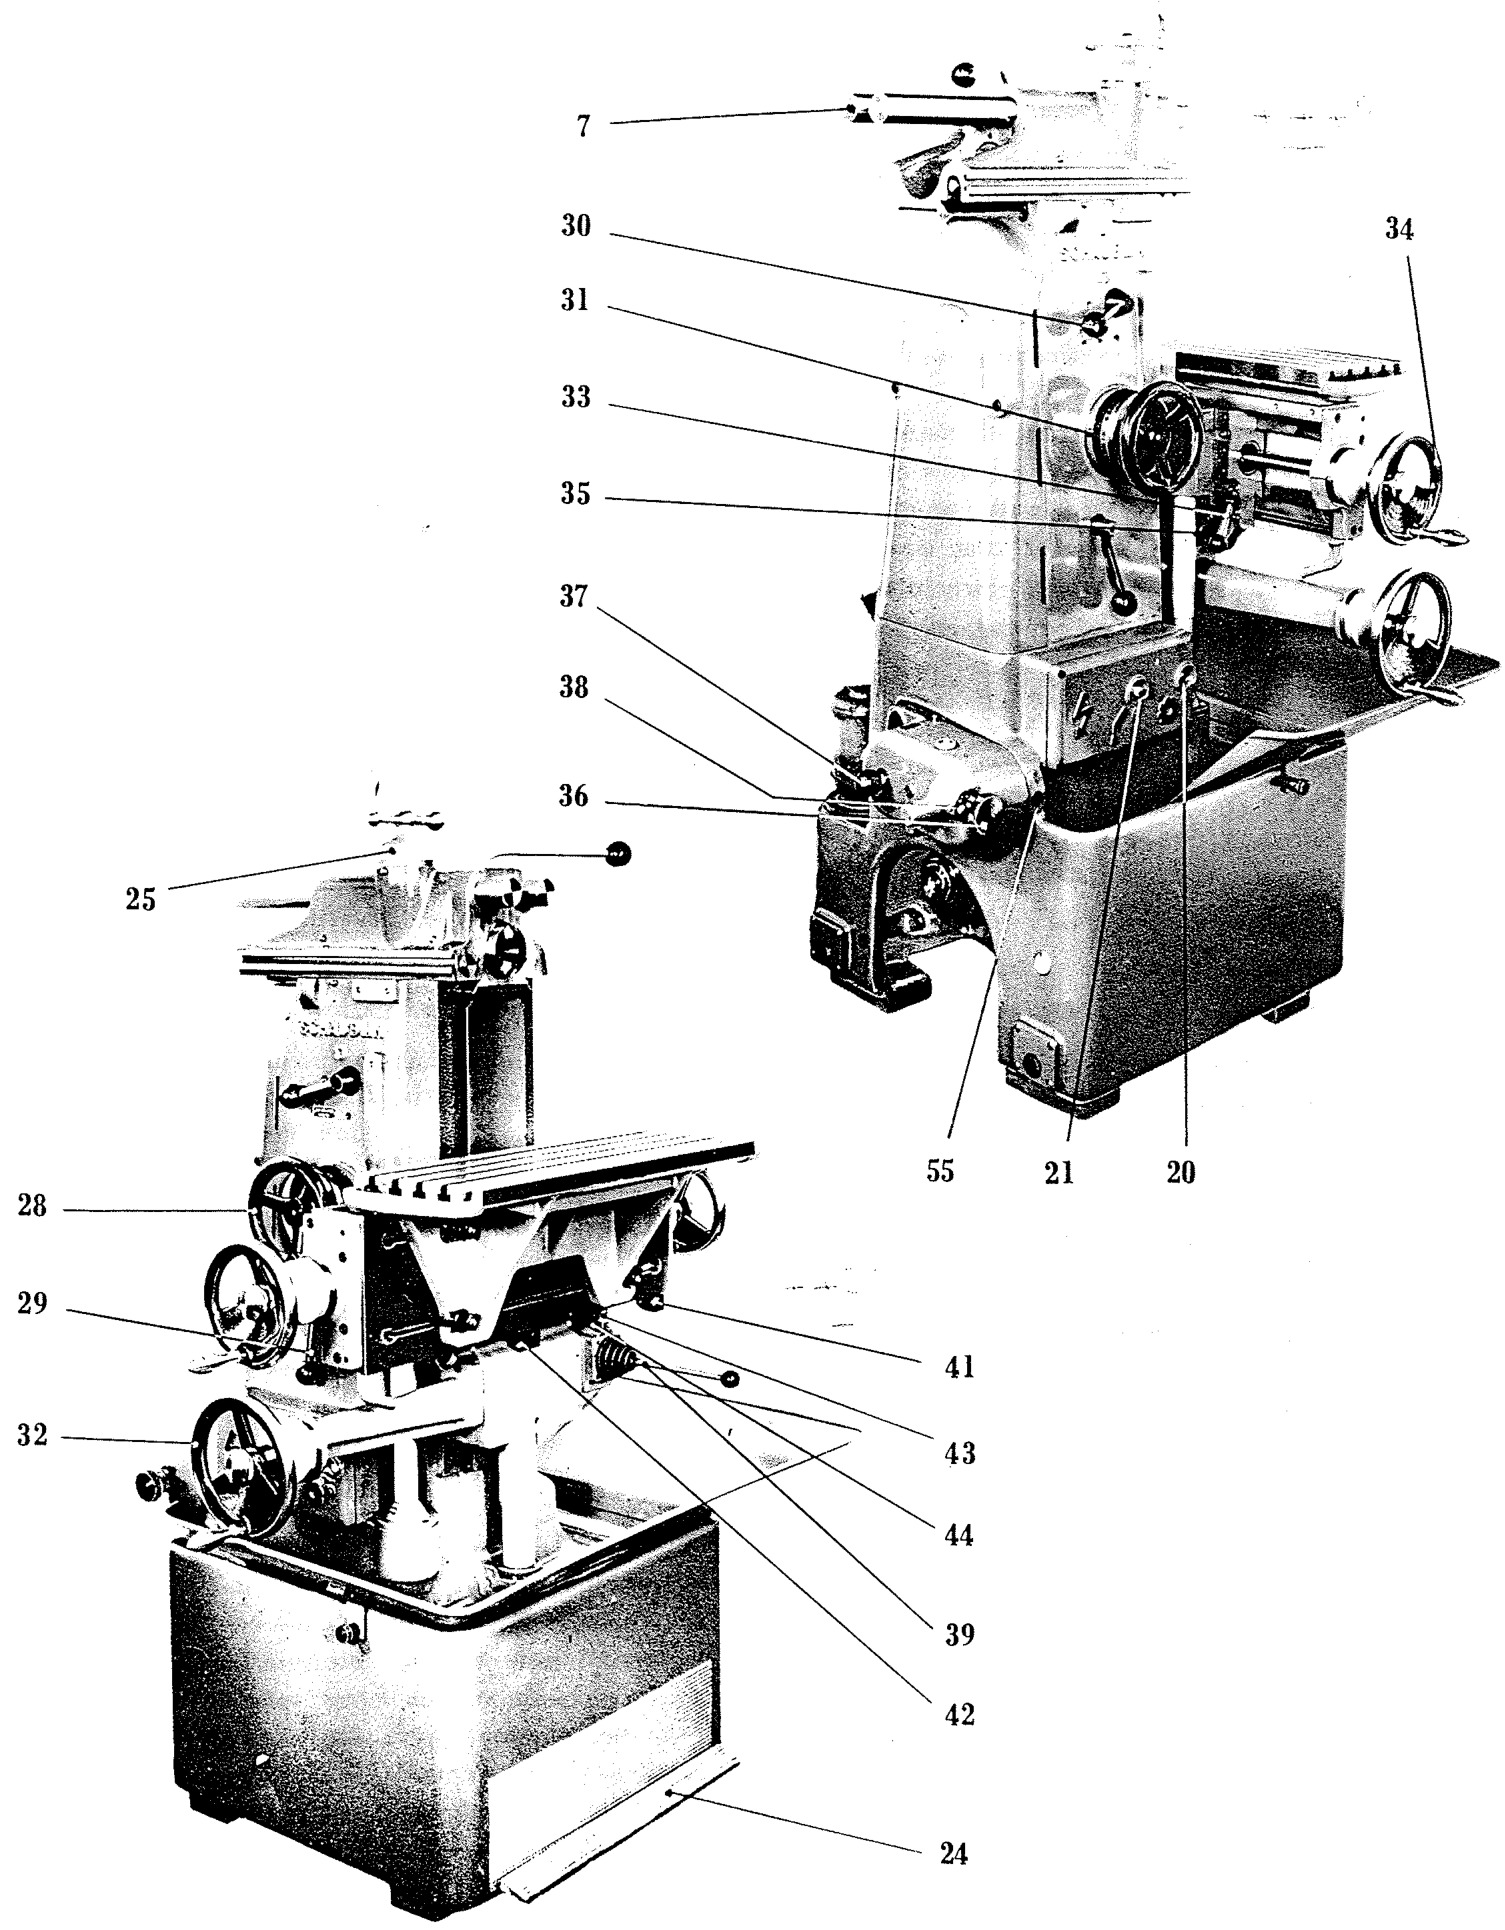
\includegraphics[width=1.0\linewidth]{./images/page_18}
    \caption{Example PNG Image}
    \label{fig:speeds_and_feeds_controls}
\end{figure}

    \chapter{Automatic Slow-motion Vertical and Long Feeds}

The feedbox, independent of the spindle speeds, enables 8 feeds
(11 to 225 mm.) to be selected by operating lever 37 and turning
knob 36. The feeds are read off the graduated ring 38 mounted on
the knob 36. By means of a patented, automatic device the running
direction of the milling spindle can be reversed (e.g., for left-
hand cutters) without reversing the feed gear, thus proventing any
wrong manipulations.

Accidents due to unforeseen overloads are prevented by a friction
clutch. The drive is transmitted from the motor to the feed gear
through a vee-belt ansvewing to the following specification:

\begin{itemize}
    \item Profile: 10 x 6
    \item Angle: \(30^\circ\)
    \item Length: 750 mm
\end{itemize}

If it is desired, for instance, to set a feed of 29 mm./min.,
knob 36 must be turned until the figure 29 is on top. The colours
on the graduated ring 38, on which the number 29 is marked,
indicate whether the lever 37 must be pushed or pulled (for 29 mm./
min. green colour; pull lever 37). Whilst the motor is running,
these operations can be performed on the lower feed range only.

The feed set in mm./min. applies both to the vertical and to the
long feed.

The automatic feed is disengaged when lever 37 is in its middle
position.

The automatic movements of the table are controlled by shifting a
single lever, 39, in the direction of the desired feed. When this
lever is shifted to the right, the table feeds to the right; when
the lever is shifted upwards, the table moves upwards. With the
lever in its middle position, the table remains stationary.


\ul{The adjustable trip blocks 40 and 41} automatically stop the table
at the desired position. For stopping the long feed, the automatic
feed is first disengaged by a portion of the head of the set
screw 42, which presses against the roller 43. Feed is then conti-
nued by hand until the set-screw 42 brings up by another part of
its head against the fixed stop 44. In this way very accurate
stoppage of the table in the desired positions is achieved.
Never remove the end-stops 40 and 41.

    {\let\clearpage\relax


\chapter{Longitudinal and Vertical High-Speed Feed}}

The high-speed feed of 1000 mm./min. is independent of the slow-
motion feeds and is actuated by a separate motor housed in the
base. A slipping clutch is provided to prevent accidents and
overloading; adjustment is not necessary. The motor switch is
operated by pressing on the pedal 24 located on the front of
the base. By means of a patented device, the high-speed feed can
be engaged even when the table is already moving. This means
that the table can be fed forward at high speed until pressure
on the pedal 24 is removed, when the table will continue to
feed forward under the actuation of the slow-motion feed gear,
no manipulation of levers being required.

    \newpage
\begin{figure}[h]
    \centering
    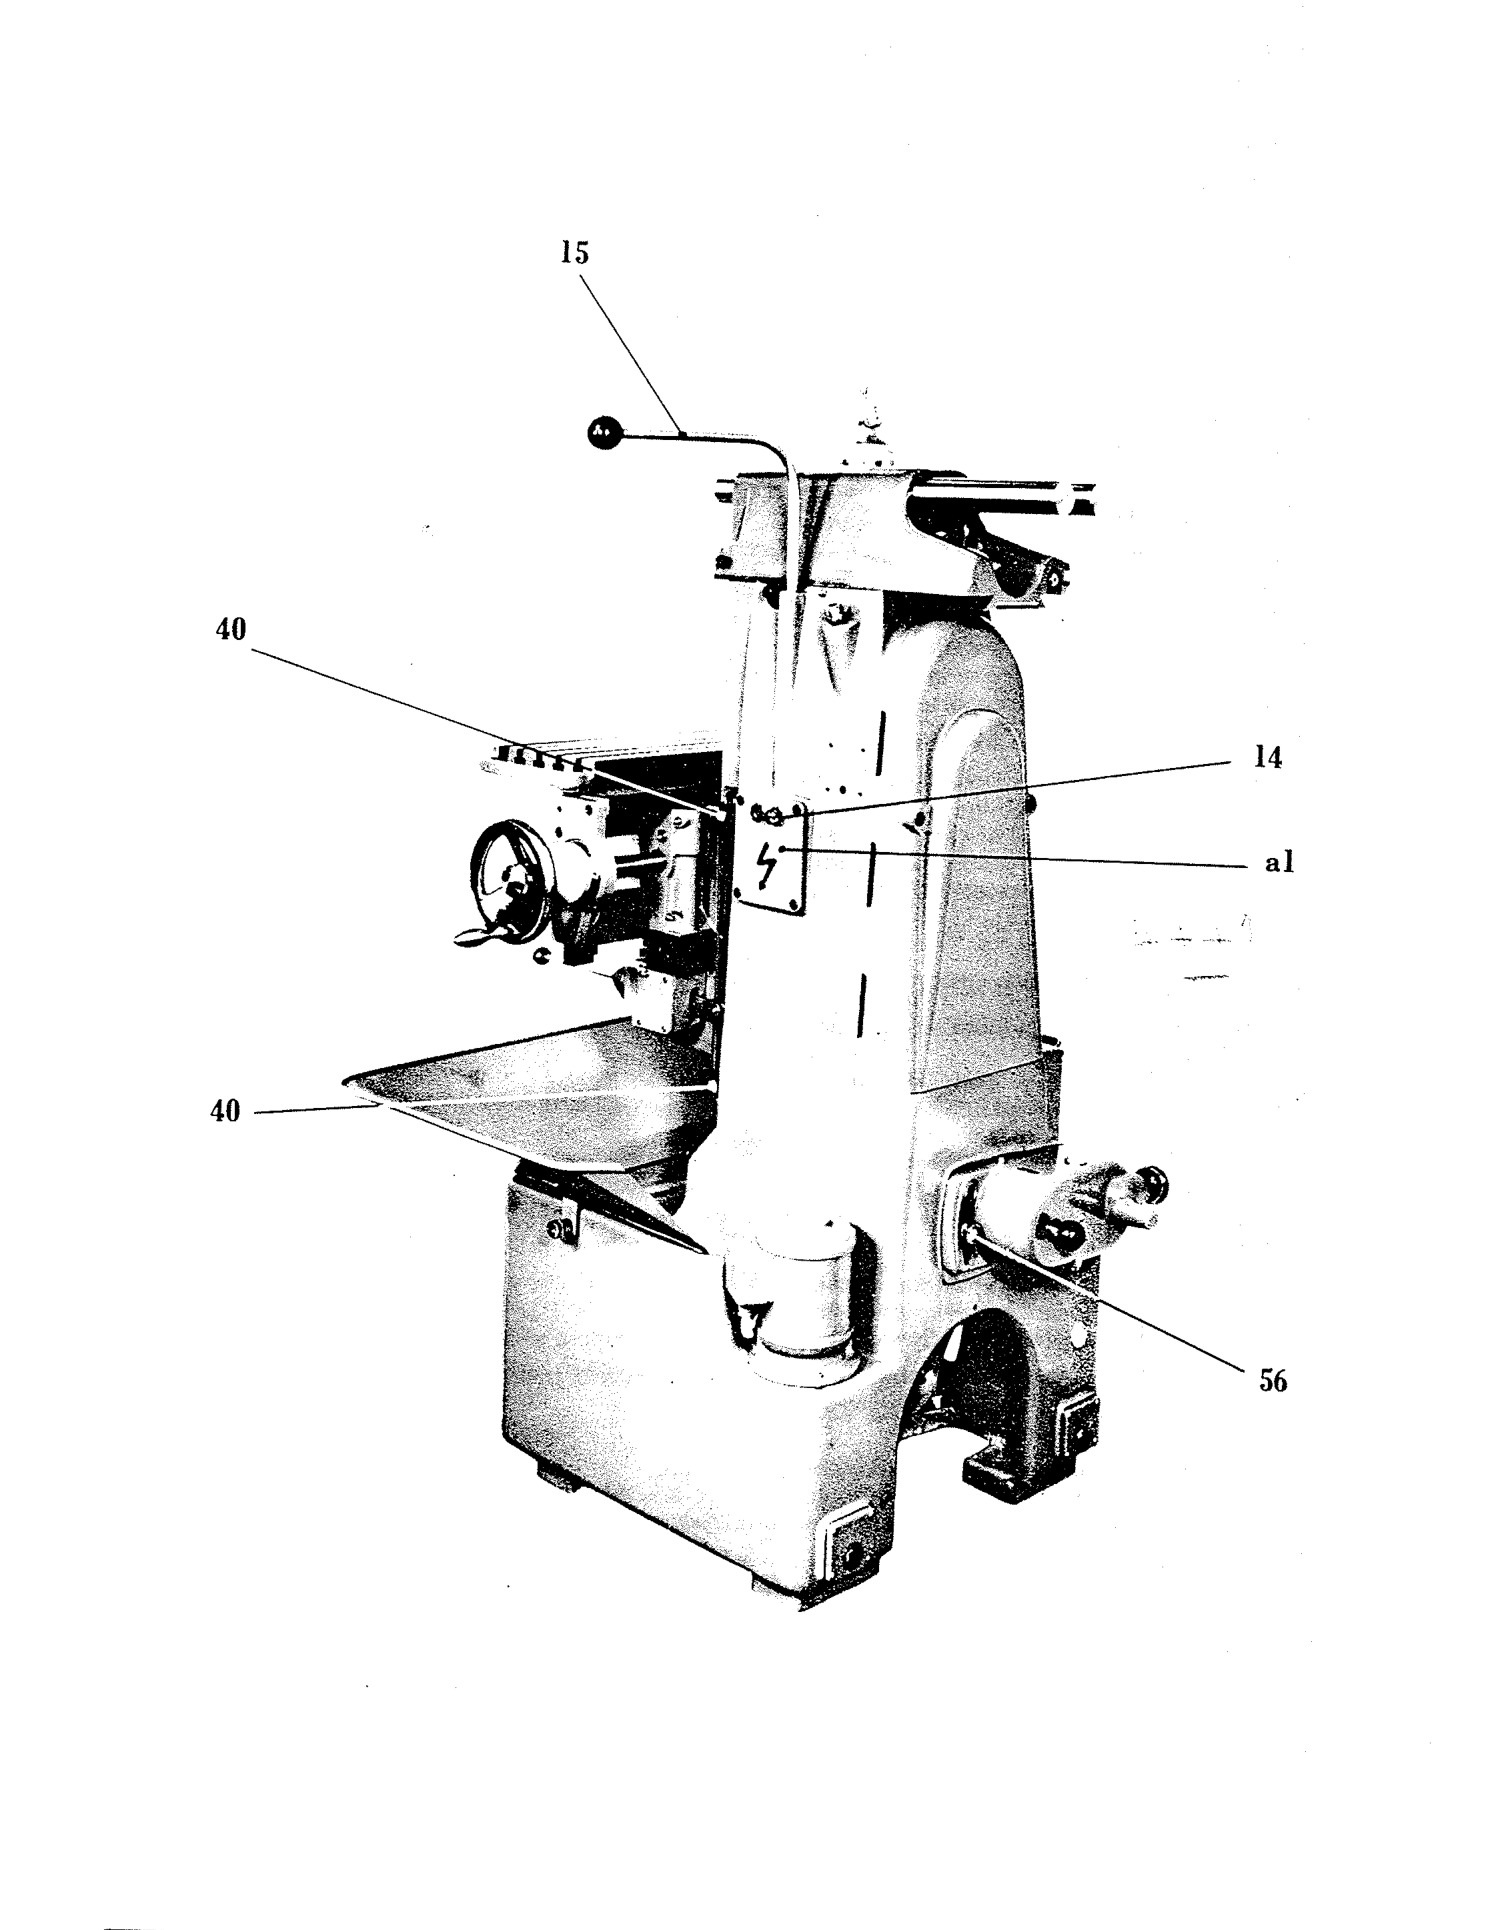
\includegraphics[width=1.0\linewidth]{images/page_20}
    \caption{Example PNG Image}
    \label{fig:speeds_and_feeds_controls_2}
\end{figure}

    \chapter{Adjustment}\label{chap:adjustments}

Only an experienced person should be entrusted with the operations of adjustment described below,
because they require the greatest of skill.

\section*{Milling Spindle Head}

\subsection*{Spindle Bearing}

The front-bearing is composed of a double row cylinder roller bearing 45, type SKF MN 3010 KX/SP

The back-bearing has two taper roller bearings 46, type 100.035 / 100.072 (accuray 2 microns) made
by La Précision Industrielle, Rueil-Malmaison (France)

These bearings are adjusted on mounting the milling machine. No readjustment is necessary until after
a long time of run.

\subsection*{Dismantling of the Spindle}

Previously the milling spindle head has to be taken off, taking into consideration the following
instructions

\begin{enumerate}
    \item Unscrew totally the set screw 57 (see page 25) and pull out the taper packing strip
    \item Remove the strip 135 after having loosened 3 screws
    \item Remove the milling spindle head towards the table, raising said head as much as possible in
\end{enumerate}

order to avoid a damage of the packing by the gear wheel.
The dismantling of the spindle is done as follows:

\begin{enumerate}
    \item Remove the coverplate 137 held by six screws
    \item Unscrew the locking screw 138
    \item Loosen screw 47 and unscrew entirely cover 48
    \item Take off nut 139 held by the safety washer on the spindle
    \item Push out carefully the spindle, striking its back-end slightly with a lead hammer
\end{enumerate}

\subsection*{Taking Up Radial Play within the front bearing}

\begin{enumerate}
    \item Determine the exact amount of radial play by means of a dial having a division of 0,001. (.00004 in.)
    \item Remove the spindle 26 (see "Dismantling the spindle")
    \item Tighten the nut 149 according to the radial play to be adjusted. A safety washer connects the ringnut 149 with the spindle.

    The slight taper of the inner race of bearing 45 obstructs a regular advance of the nut 140.
    To obtain the desired result, the nut should be struck concentrically by means of a tube placed
    on the spindle to cause a slight displacement of the inner race of the bearing 45 on the taper
    of the spindle 25, and nut 140 then retightened. By repeating this operation several times it will
    be found possible to turn nut 140 through the desired angle. Keep a careful check on the advance
    of mut 140, as it is difficult to restore the inner race of the bearing 45 if it is once moved
    too far forward on the taper.

    The advance of nut 140 is calculated, in respect of the radial play which has to be adjusted,
    as follows:

    \ul{Advance of nut 140 = bearing play to be adjusted in mm x 14}
    Pitch of nut 140 = 1,5 mm.

    \ul{Example:} A radial play of 0,01 mm has to be adjusted.
    Advance of nut 140 = 0,01 mm x 14 = 0,14 mm or a rotation of 36° 36' corresponding to a length
    of 20,5 mm on the full diameter of nut 140 (diam. 70 mm).

    \item Lock the nut 140 by means of the safety washer
    \item Replace spindle 26 and test again the radial play of the front-bearing; it should be 0,002 mm
    (.00008") in order to obtain faultless running conditions. This test shall be made with ball
    bearings 46 in position and with roller bearing 45 absolutely dry.
\end{enumerate}

\subsection*{Taking up radial and axial plain in the rear-bearing}

\begin{enumerate}
    \item Loosen screw 47
    \item Screw in the cover 48 (pitch 1,25 mm) according to the amount of play which has to be adjusted
    \item Firmly tighten screw 47 and test again the axial play of the back-bearing; it should be 0,01 mm
    (.0004") to obtain faultless running conditions. This test shall be done with taper roller bearings
    46 absolutely dry.
\end{enumerate}

    \newpage
\begin{figure}[h]
    \centering
    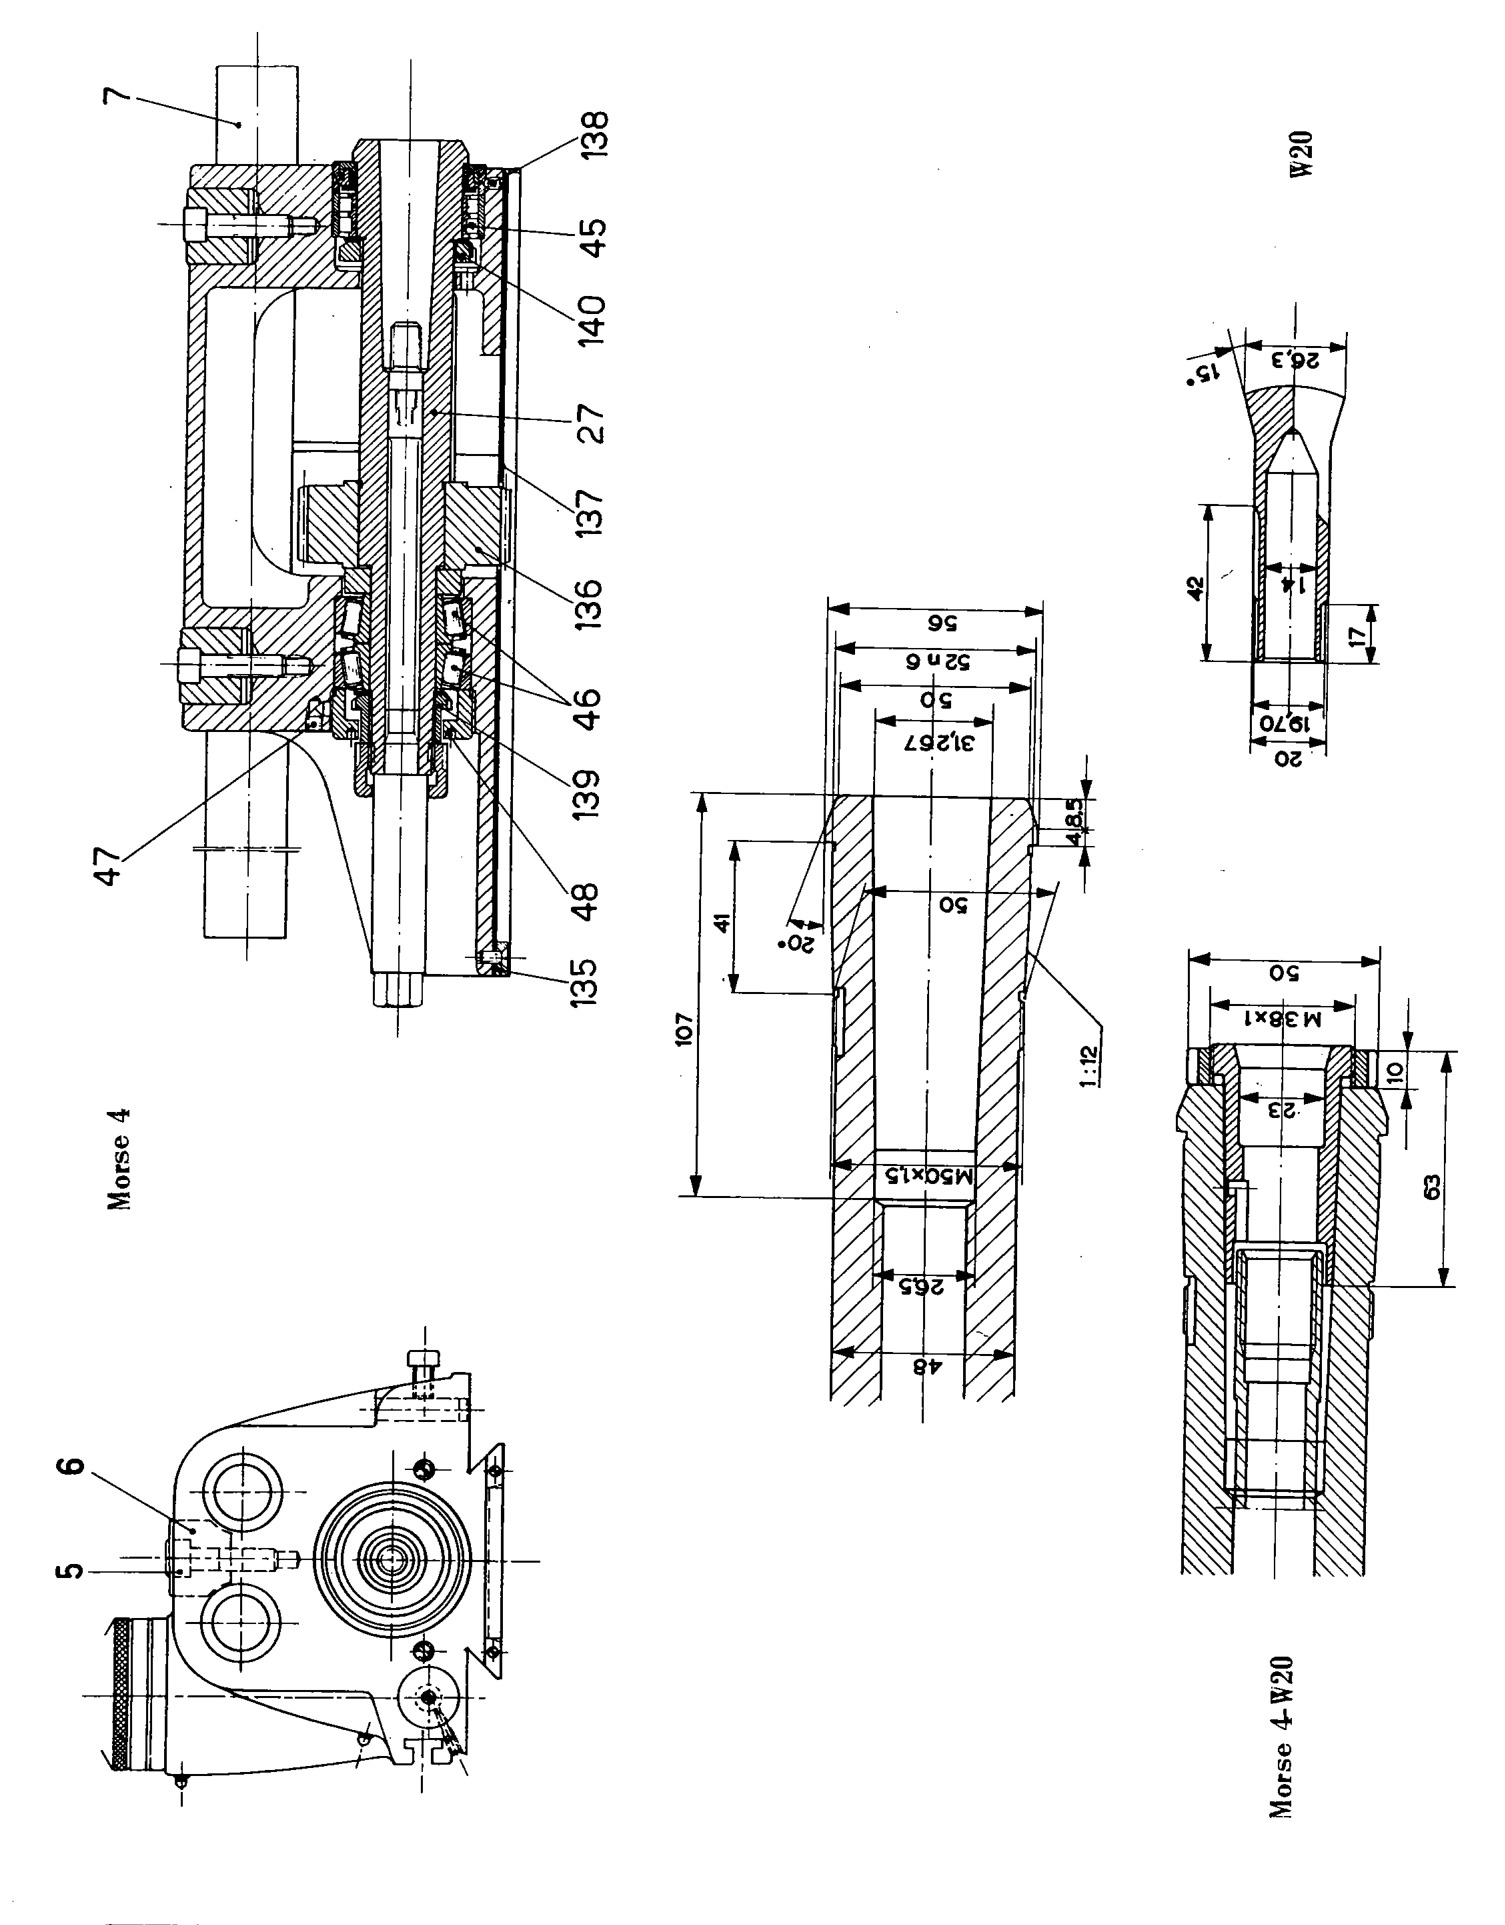
\includegraphics[width=1.0\linewidth]{./images/page_22}
    \caption{Example PNG Image}
    \label{fig:horizontal_spindle_dimensions_1}
\end{figure}

    \newpage
\begin{figure}[h]
    \centering
    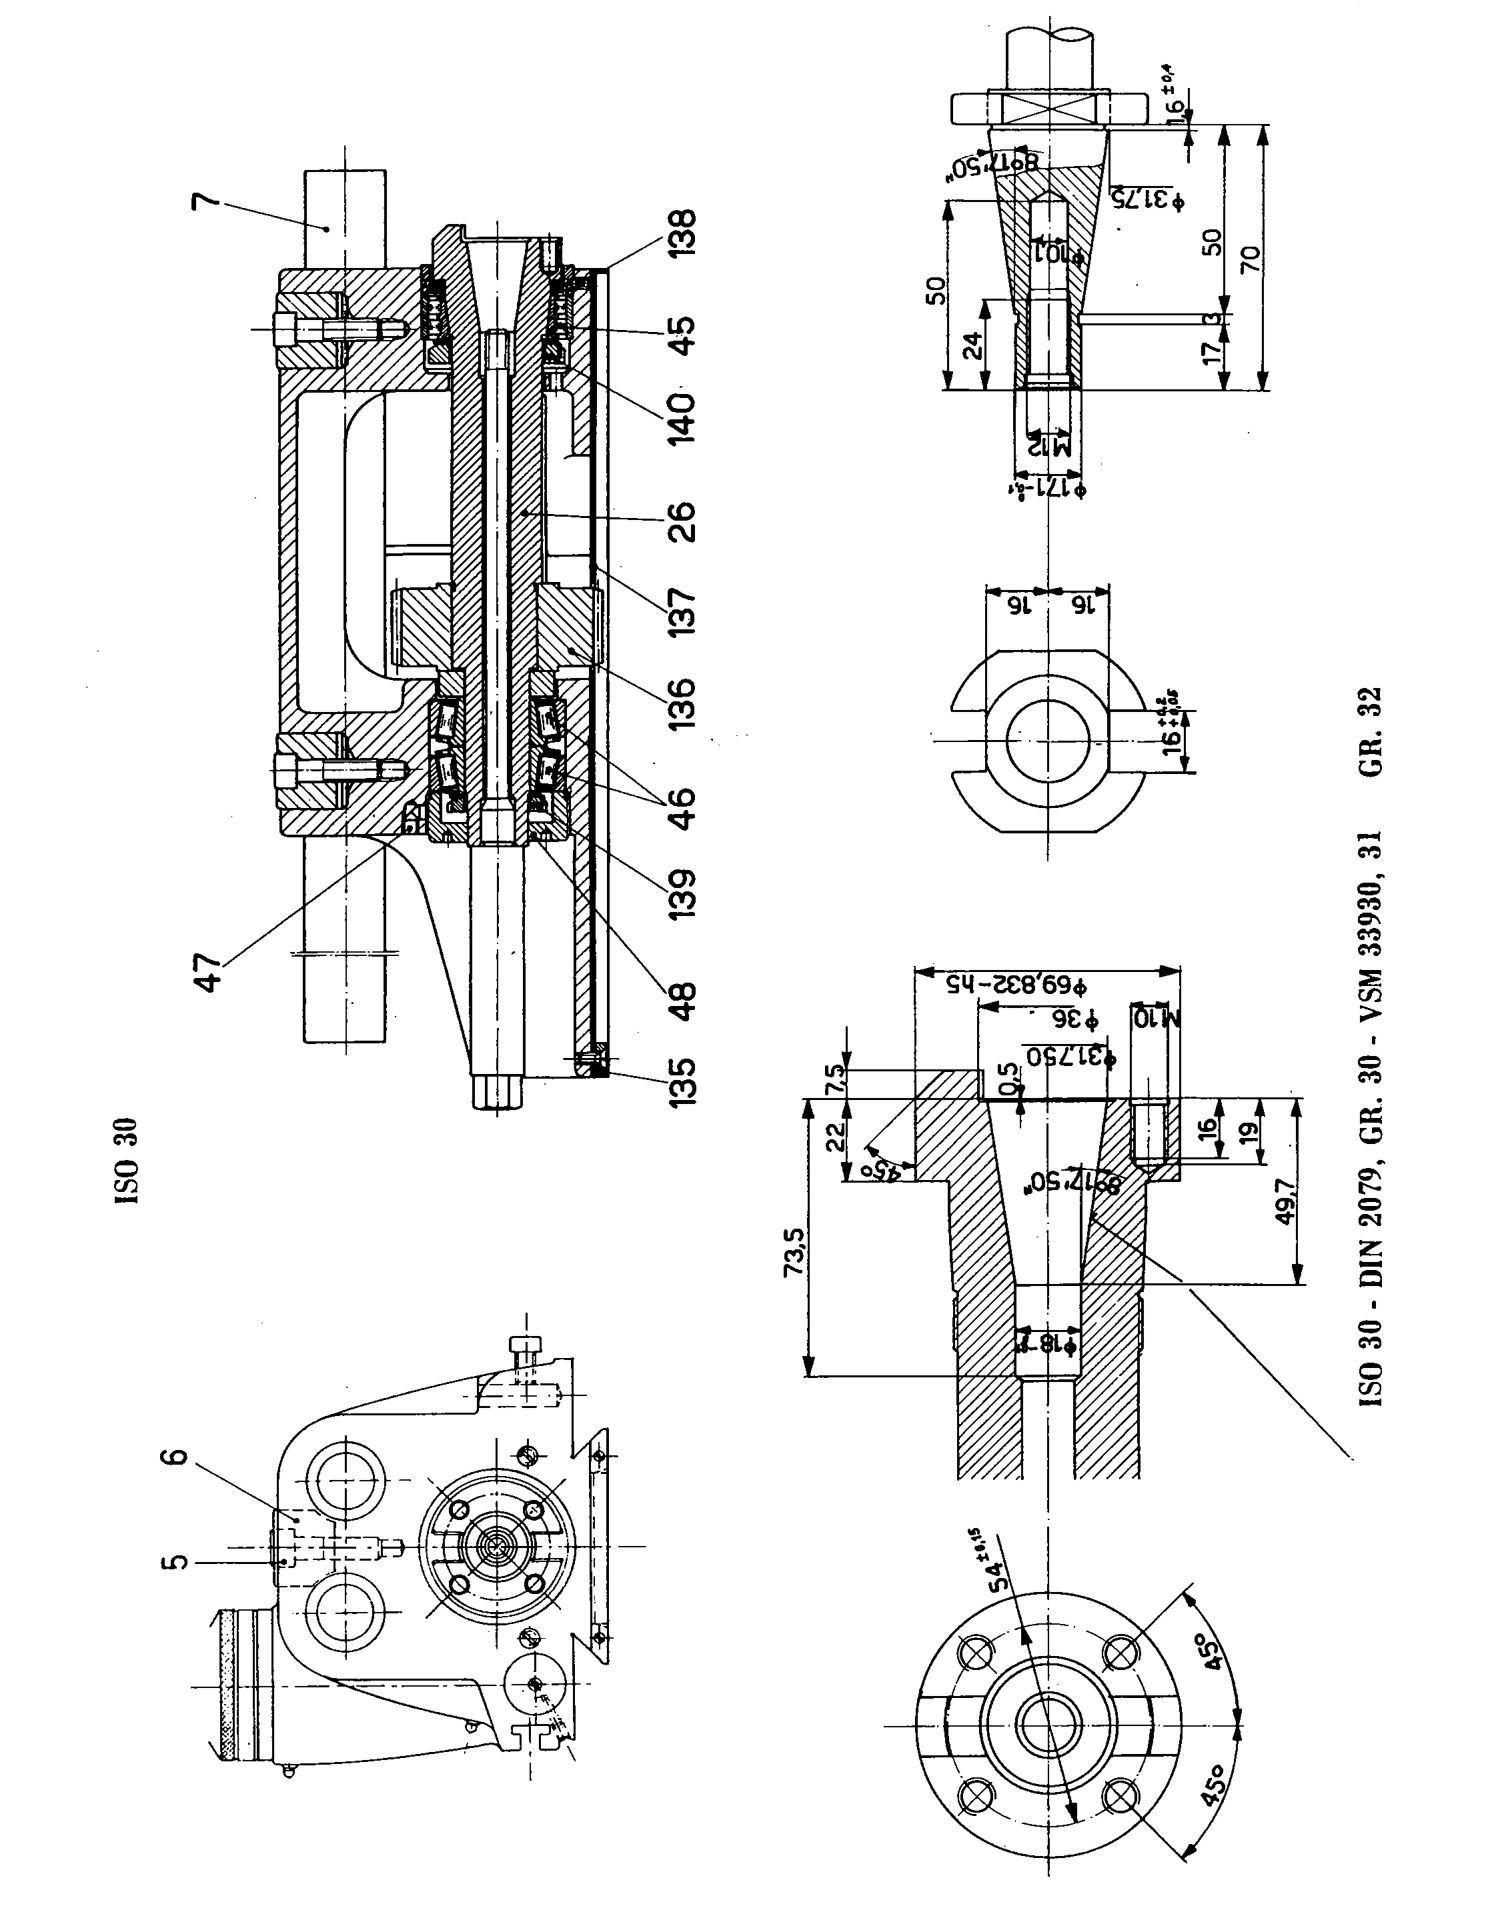
\includegraphics[width=1.0\linewidth]{images/page_23}
    \caption{Example PNG Image}
    \label{fig:horizontal_spindle_dimensions_2}
\end{figure}

    \chapter{Spindle Speed Variator}\label{chap:spindle_speed_variator}
\section*{Adjustment of Belt Tension}
Adjust the higher speed, i.e., 2000 rpm, using the handwheel 28.

\subsection*{Upper Belt:}
\begin{enumerate}
    \item Loosen the two screws 49.
    \item Tighten the belt by pulling the support downward. To ensure that the spindle speed corresponds to that on the dial (2000 rpm), a belt withdrawal of 1 mm from the outer diameter should be observed.
    \item Tighten the two screws 49.
\end{enumerate}

\subsection*{Lower Belt:}
\begin{enumerate}
    \item Unscrew the nut 50.
    \item Tighten the belt by screwing the nut 51. To ensure that the spindle speed corresponds to that on the dial (58 rpm), a belt withdrawal of 1 mm from the outer diameter should be observed.
    \item Tighten the nut 50.
\end{enumerate}

{\let\clearpage\relax \chapter{Feed Box}}

\section*{Belt Tension Adjustment}

\begin{enumerate}
    \item Loosen the 2 screws 55 \& 56.
    \item Tilt the box upward to tighten the belt.
    \item Tighten the two screws 55 \& 56 (see page \pageref{fig:speeds_and_feeds_controls} \& \pageref{fig:speeds_and_feeds_controls_2}).
\end{enumerate}

    \newpage
\begin{figure}[h]
    \centering
    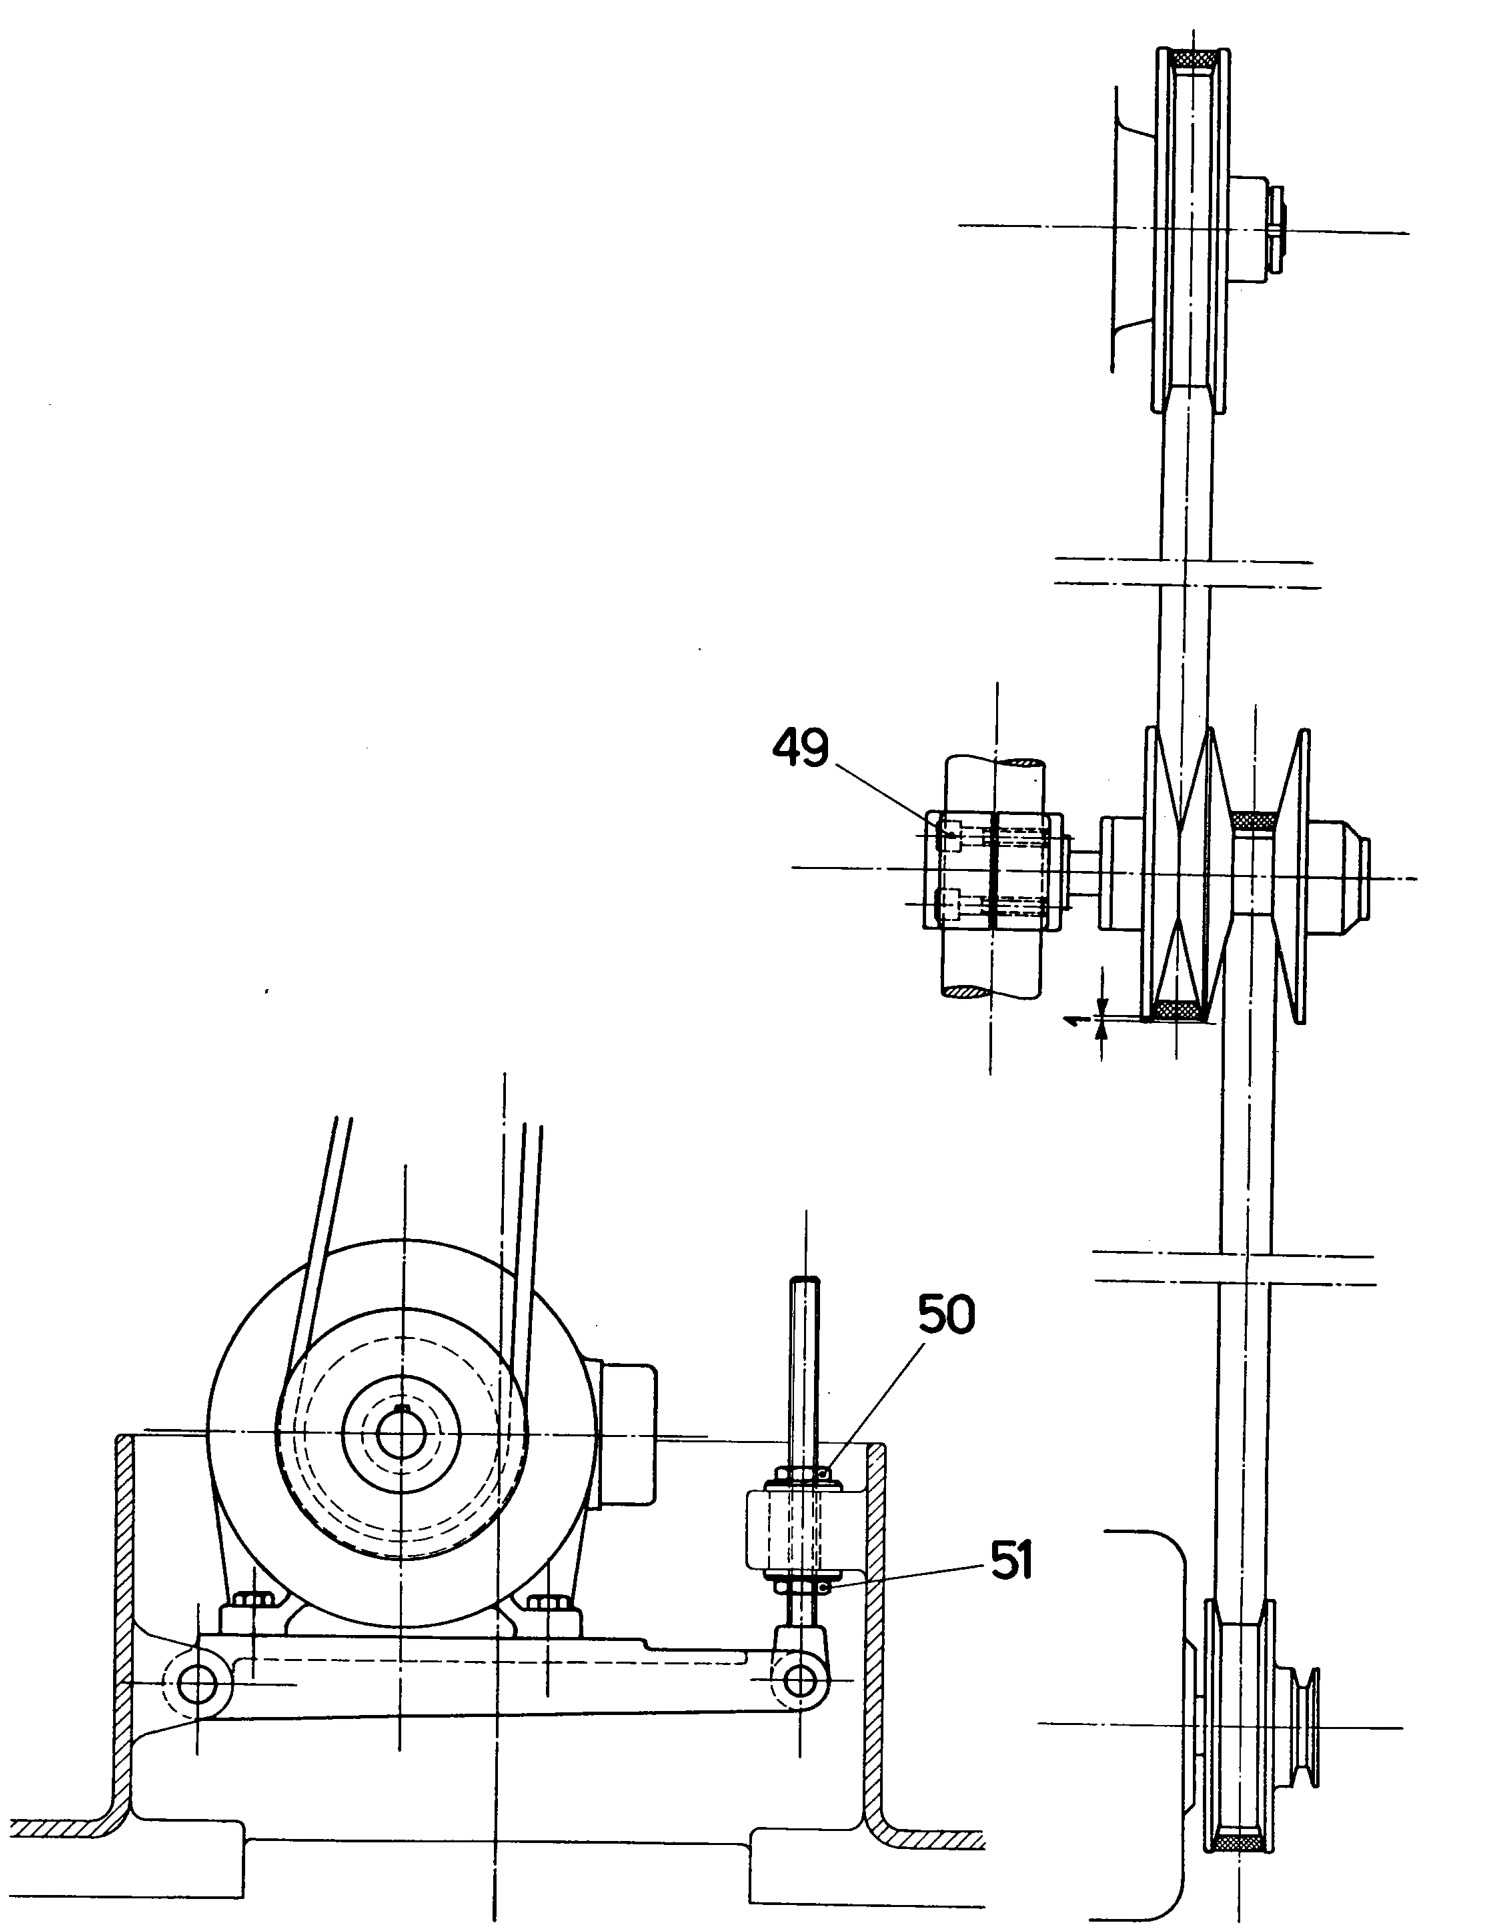
\includegraphics[width=1.0\linewidth]{./images/page_25}
    \caption{Example PNG Image}
    \label{fig:belt_tensioning}
\end{figure}

    \chapter{Adjustment}\label{chap:adjustment}

\section*{Adjustment of Conical Gibs}

The spindle head, vertical, and longitudinal slides are equipped with conical gibs for backlash compensation. The adjustment is done simply by the screw 57. See page \pageref{fig:handwheel_bearings}, position A.

\section*{Compensation of Axial Play of the Transverse Screw (spindle head)}

\begin{enumerate}
    \item Remove the screw 58.
    \item Screw an M6 bolt into the same hole and thus remove the cover 59.
    \item Screw the nut 60, locked by the lock washer 61, according to the amount of play to be compensated, which has been previously determined by precise control. See page \pageref{fig:handwheel_bearings}, position B.
\end{enumerate}

\section*{Compensation of Axial Play of the Longitudinal Screw}

\begin{enumerate}
    \item Loosen the 2 screws 62.
    \item Screw the nut 63 according to the amount of play to be compensated, which has been previously measured by precise control.
    \item Tighten the screws 62.
    See page \pageref{fig:handwheel_bearings}, position C.
\end{enumerate}

\section*{Compensation of Axial Play of the Vertical Screw}

\begin{enumerate}
    \item Unscrew the knob 64 and the nut 64a.
    \item Remove the freed parts.
    \item Loosen the screw 65.
    \item Lock the nut 66 (pitch 1 mm) according to the amount of play to be compensated, which has been previously determined by precise control.
    \item Lock the screw 65.
    See page \pageref{fig:handwheel_bearings}, position D.
\end{enumerate}


    \newpage
\begin{figure}[h]
    \centering
    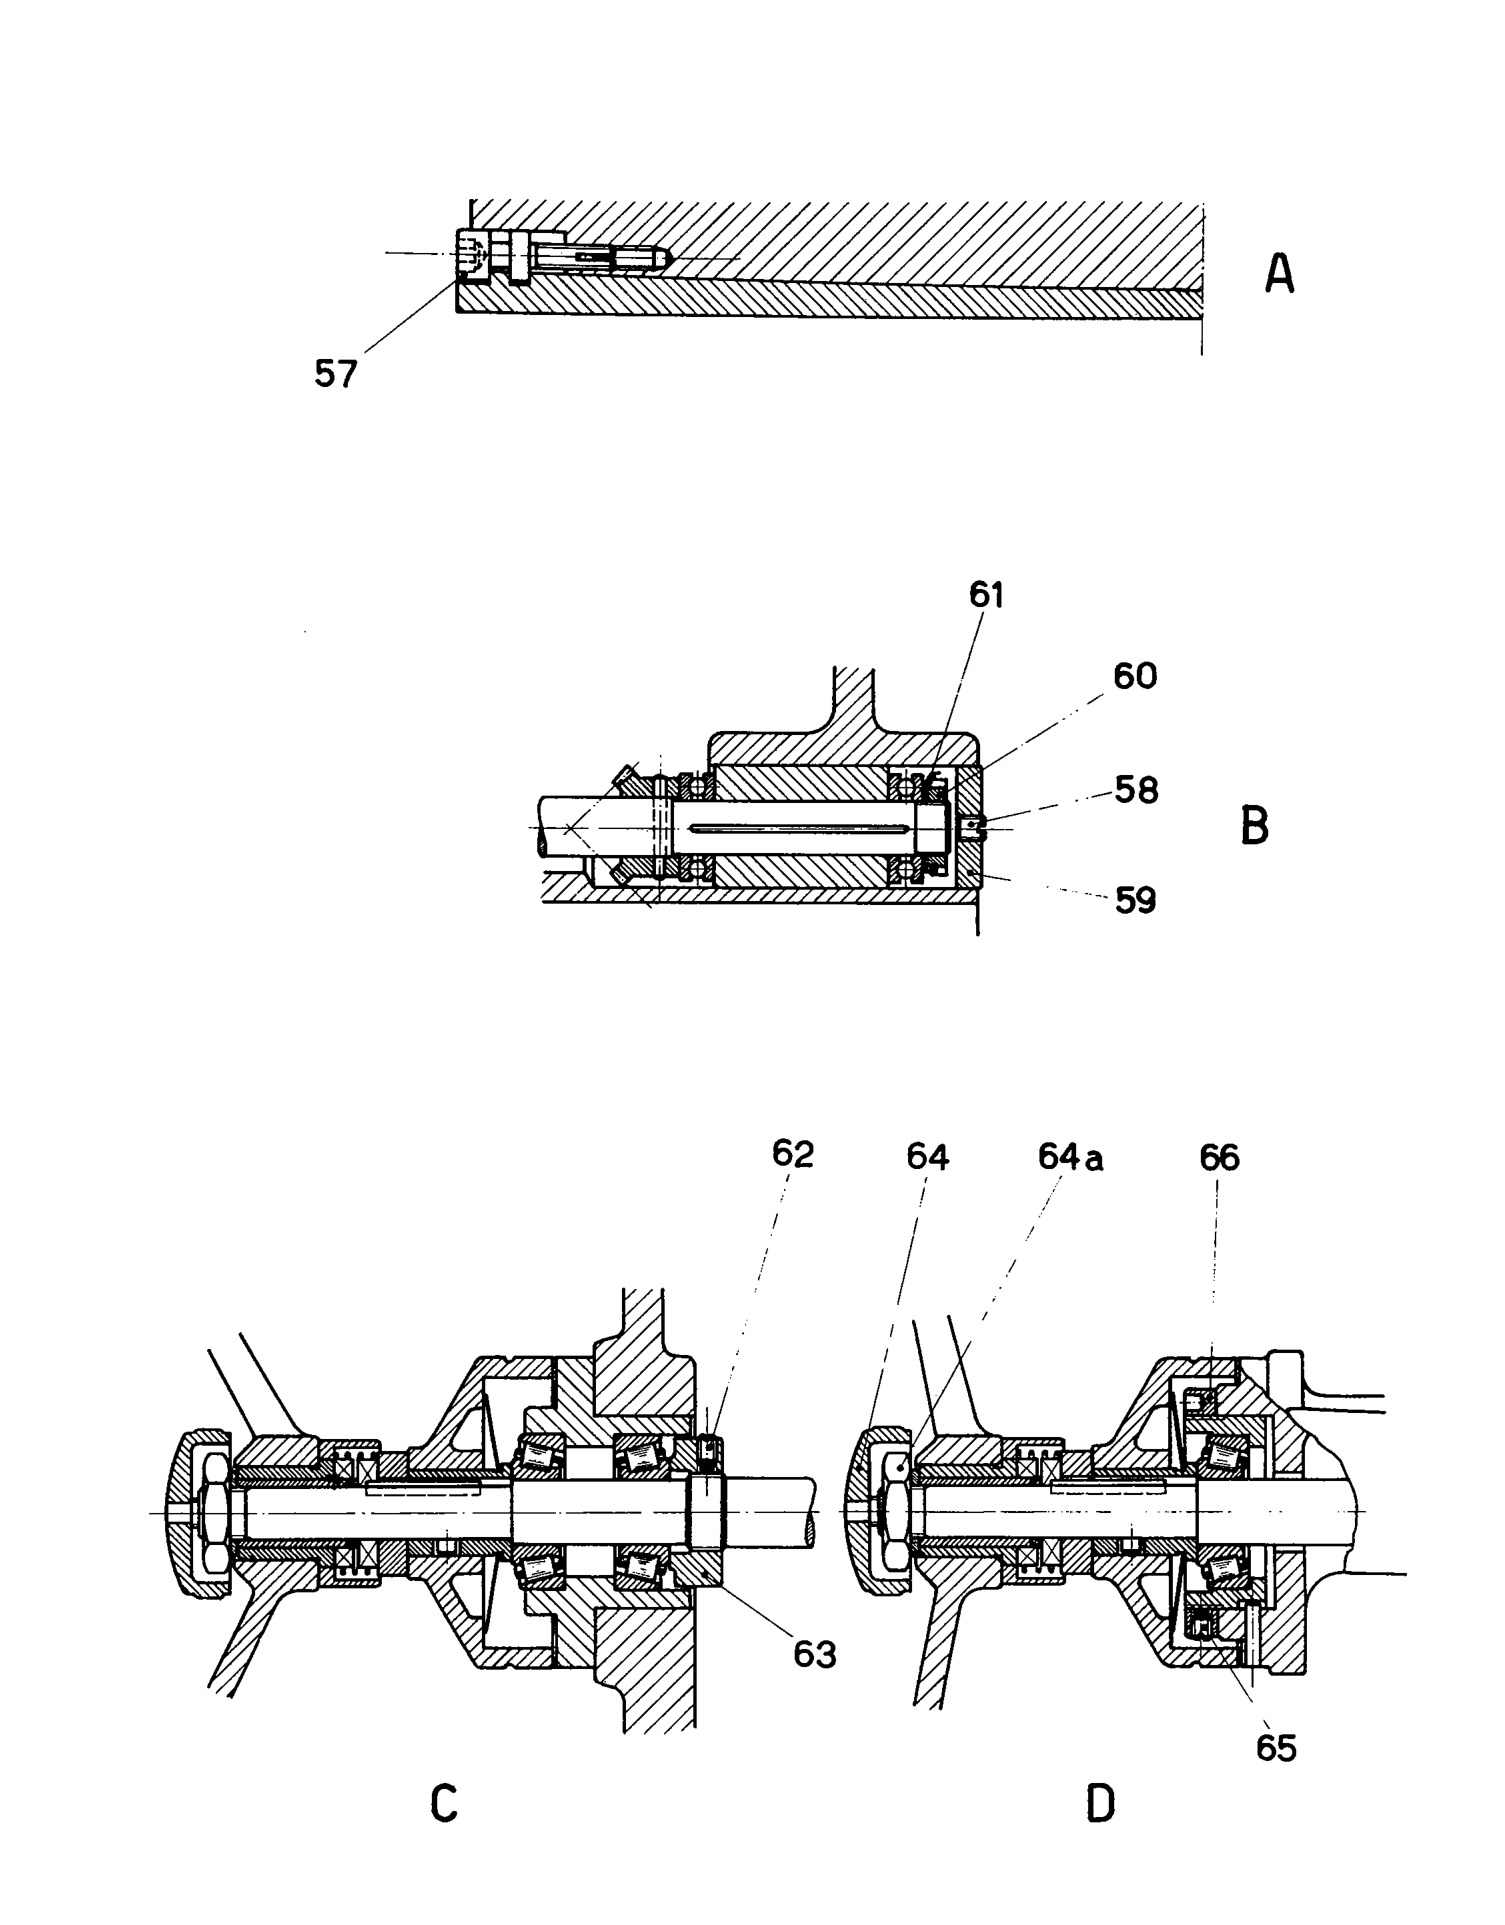
\includegraphics[width=1.0\linewidth]{./images/page_27}
    \caption{Example PNG Image}
    \label{fig:handwheel_bearings}
\end{figure}

    \chapter{Cooling System}

The cooling system circuit is given on page \pageref{fig:cooling_system}.

The reservoir 67 is located inside the base and forms a single piece with it. When filled to the middle of the level indicator 68, it contains approximately 24 liters of liquid.

The motor-pump unit 18 is mounted outside the machine, making it easily accessible for cleaning. The liquid supply pipe passes through the frame. The nozzle of the flexible tube that delivers the lubricant to the cutter is held in a good position by a support 69 mounted on the spindle head. The valve 70 allows adjusting the liquid flow.

The pump, reservoir, as well as pipes, filters, etc., are cleaned periodically (see ANNEX-1 attached). The two plugs 71 allow draining, and the two covers 72 allow cleaning the reservoir. The liquid drainage occurs in all table positions through two flexible hoses.

When the pump cooling is not required, a bucket can be attached to the support 69.

\textbf{RECOMMENDATION:}

Experience has shown that it is \underline{preferable to use a good cutting or turning oil as a lubricant}.

Soluble oils, decomposing after prolonged use, can cause corrosive actions on the machine components.

    \newpage
\begin{figure}[h]
    \centering
    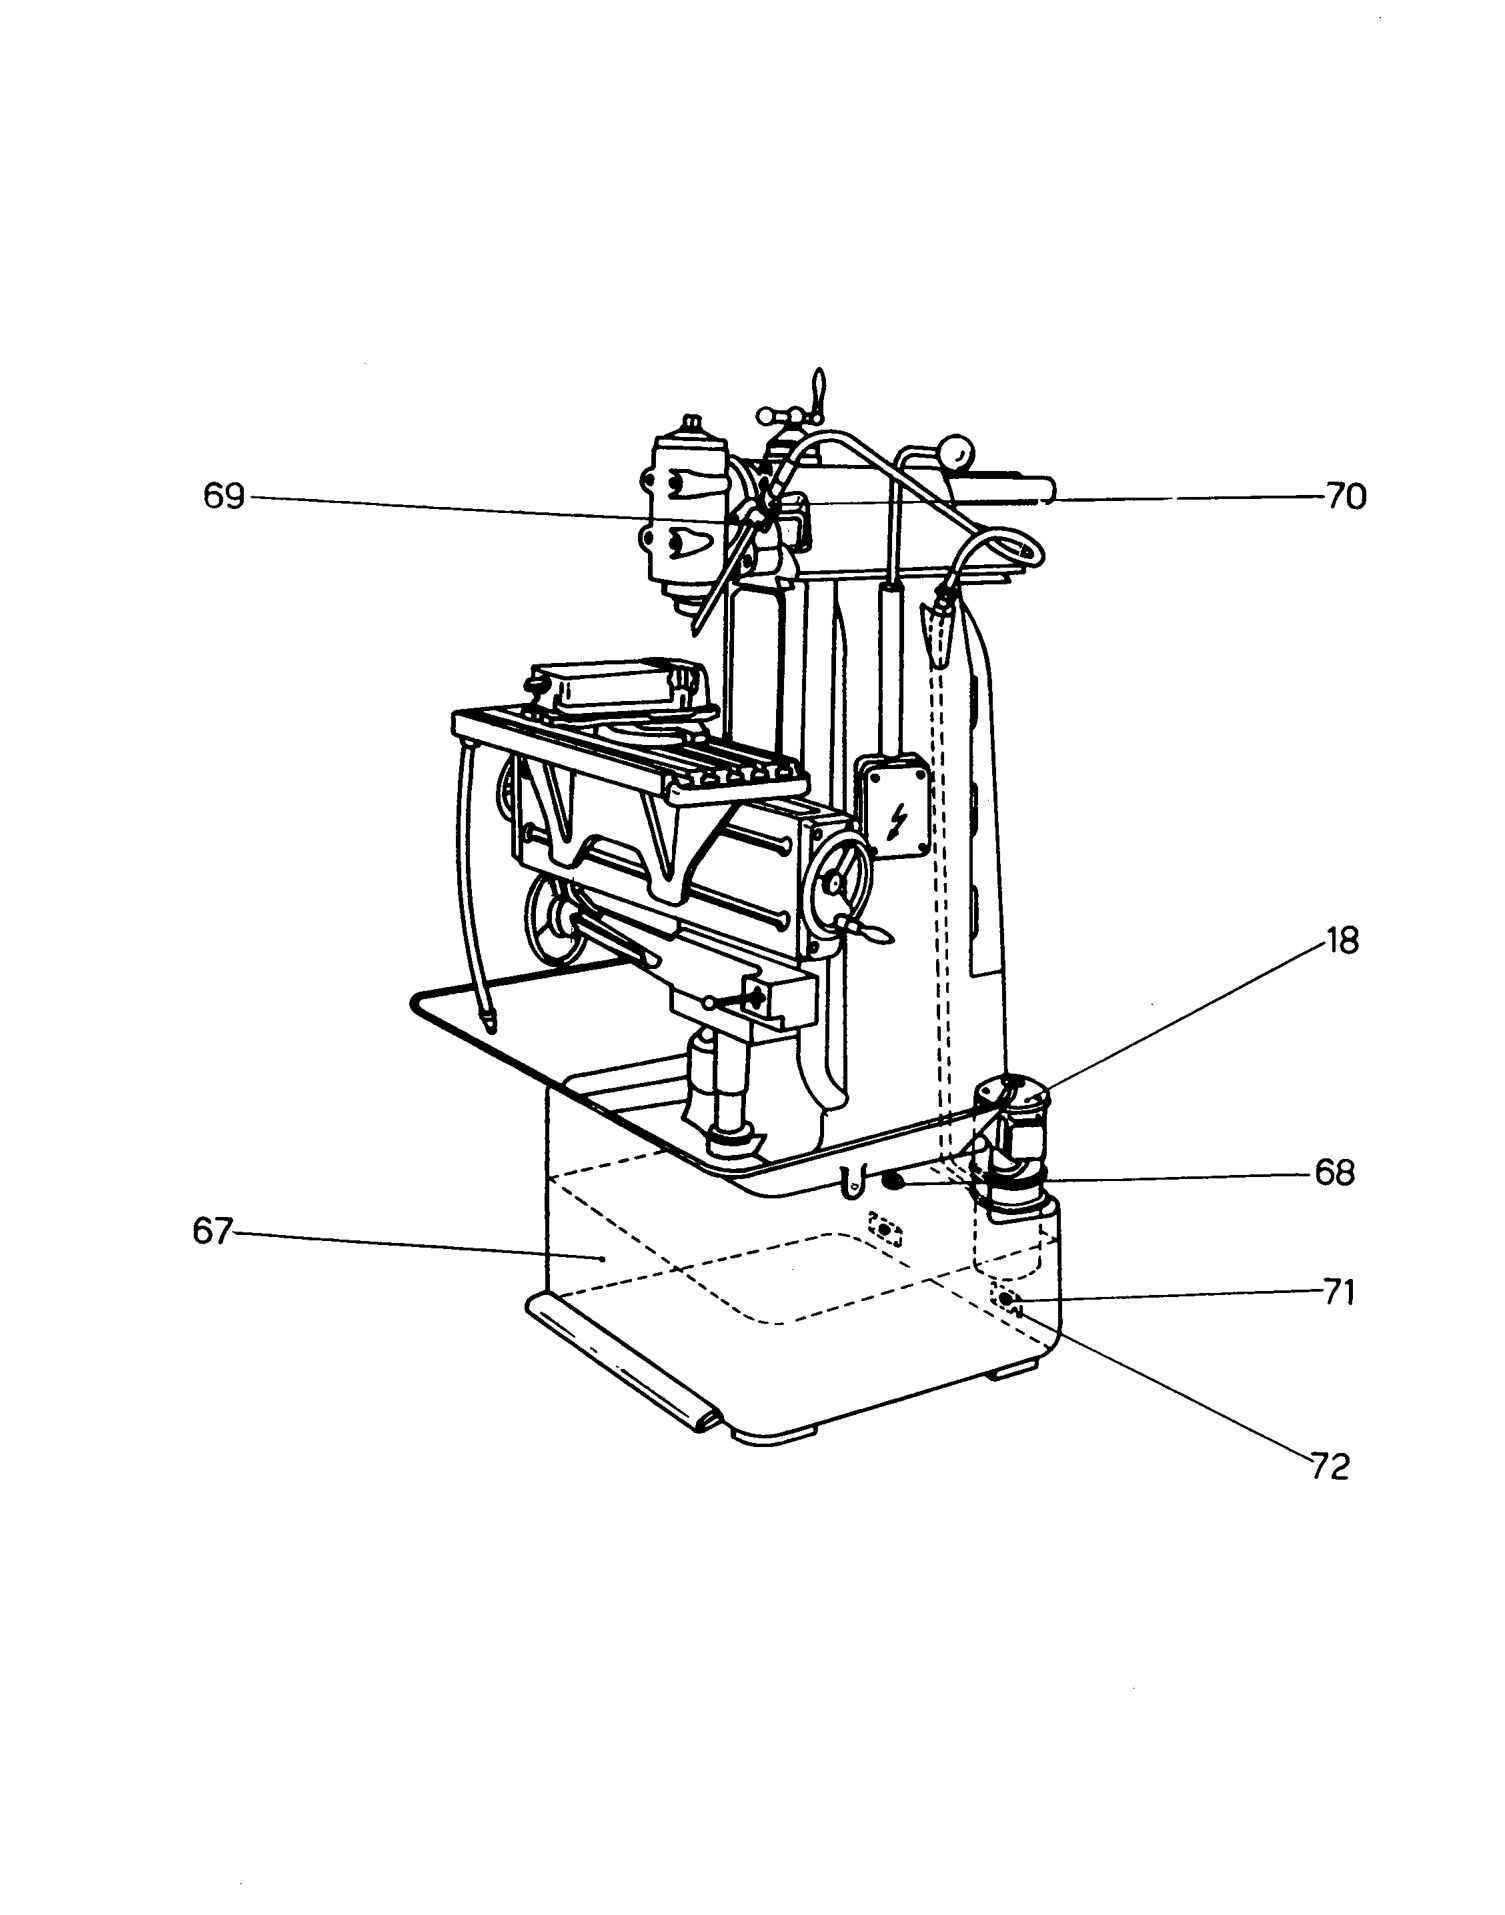
\includegraphics[width=1.0\linewidth]{images/page_29}
    \caption{Example PNG Image}
    \label{fig:cooling_system}
\end{figure}

    \chapter{Accessories Normally Supplied with the Machine}

\begin{enumerate}
    \item Clamping key
    \item Milling arbor $\varnothing$16x97 mm
    \item Milling arbor block $\varnothing$22x37 mm
    \item Counter-support with 2 guide bushes
    \item Waco oil syringe
    \item 4 Hex keys for internal hexagon from 4 - 6 - 8 - 10 mm
    \item 1 Hex key for internal hexagon of 5 mm for quick-change head and indexer
    \item 1 22 mm open-end wrench
    \item 2 Open-end wrenches of 14 \& 17 mm for the indexer.
\end{enumerate}

    \appendix


\chapter{Instructions for Use of the 950 Rotary Table on the Schaublin 13 Universal Milling Machine}

\section*{Main Features}

\begin{tabular}{@{}ll@{}}
    Table Diameter          & 250 mm      \\
    Total Height            & 90 mm       \\
    Inner Cone of the Table & Morse 2     \\
    Table Division          & Every 0° 1' \\
    Number of T-Slots       & 8           \\
\end{tabular}

\begin{figure}[h]
    \centering
    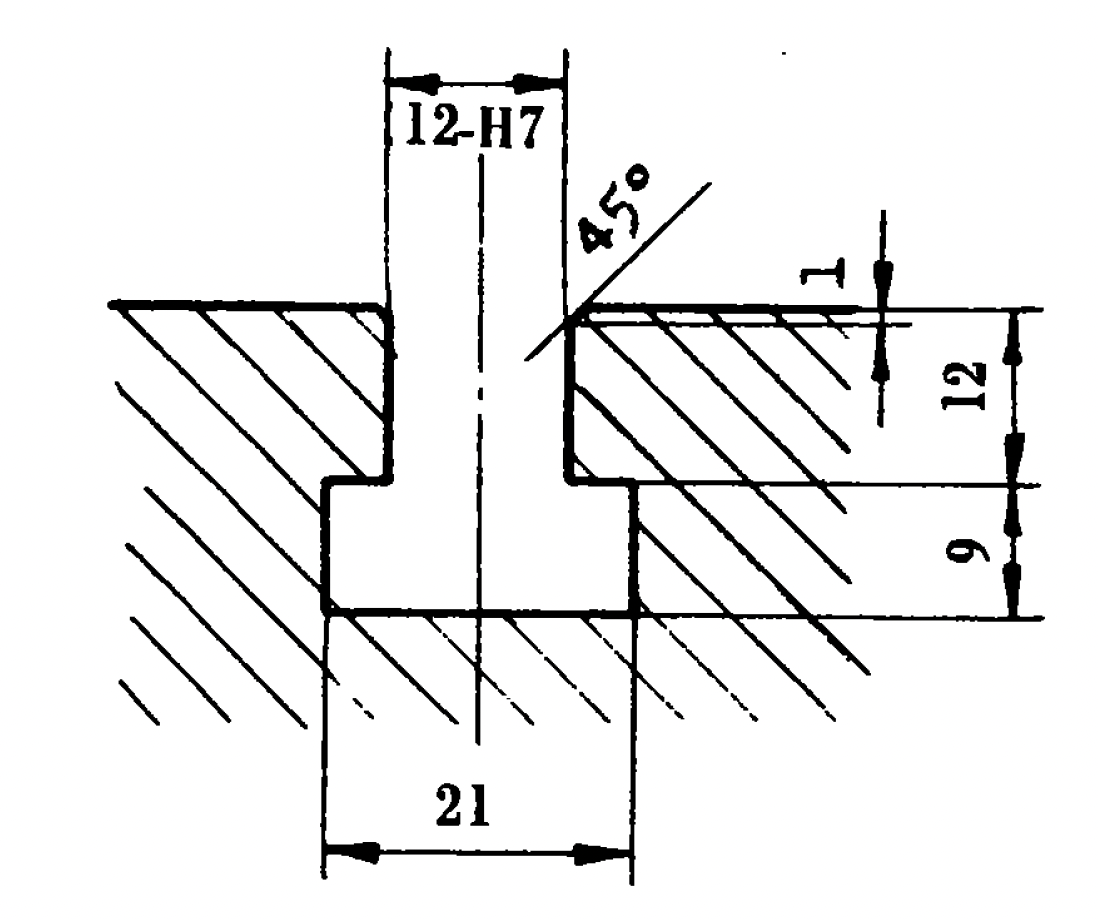
\includegraphics[width=0.6\linewidth]{images/rotary_table_t_slot_dimensions}
    \caption{T-Slot Dimensions \& According to VSM 33811}
    \label{fig:rotary_table_t_slot_dimensions}
\end{figure}


\section*{Accessory}

\begin{tabular}{@{}ll@{}}
    1050 & 3-disc dividing head with holes fitting on the rotary table. \\
    & Division: 2 to 360°                                          \\
    & \sout{Table of divisions: See IN 53-27 attached.}
\end{tabular}

\begin{notebox}
    Table of divisions is not included since online calculators can be used.\\
    The table has a 120:1 gear ratio.
    It comes with 3 plates with 15, 16, 17, 18, 19, 20, 21, 23, 27, 29, 31, 33, 37, 39, 41, 43, 47 and 49 holes.
\end{notebox}

The table is secured on two T-slots of the table using 4 bolts $\varnothing$10 provided with this accessory.
Two guide stones ensure its alignment on the table. Two eccentric locks immobilize the table.

To release the table from the worm, loosen screw 94 and turn eccentric sleeve 95 (see page 41). % TODO: add page reference

    \newpage
\section*{Cleaning, Lubrication, and Maintenance}

Upon receipt and during use, the general instructions provided for the machine must be followed.
Do not lift this accessory by its plate but by its base.

\subsection*{Oil Bath}
The worm screw is lubricated by an oil bath.
The filling is done as follows with an oil viscosity of \(3^\circ \mathrm{E}\) at \(50^\circ \mathrm{C}\):
\begin{enumerate}[label=\arabic*.]
    \item Unscrew the plug 96 and fill up to the middle of the level indicator 97.
    \item Once a year, drain and renew the oil after rinsing with petroleum.
\end{enumerate}
The plate also includes 2 oilers for pressure lubrication using the pump supplied with the machine.

\subsection*{Disassembly of the Vernier}
\begin{enumerate}[label=\arabic*.]
    \item Unscrew the screw 98.
    \item Remove the handle 99, the socket 100 carrying the vernier 101, and its spring 102.
\end{enumerate}

\subsection*{Disassembly of the Hole Discs}
\begin{enumerate}[label=\arabic*.]
    \item Unscrew the nut 103 and remove the washer 104.
    \item Remove the handle 105 carrying the piston 106 and the socket 107.
    \item Remove the needles 108 and 109.
    \item Unscrew the 3 screws 110 and remove the disc 111.
\end{enumerate}

\subsection*{Axial Clearance Adjustment of the Worm Screw}
If the axial clearance comes from the teeth:
\begin{enumerate}[label=\arabic*.]
    \item Unscrew the screw 112 completely.
    \item Unscrew the screw 113 according to the importance of the clearance to be adjusted.
    \item Put back the screw 112 and tighten it firmly.
\end{enumerate}

If the axial clearance comes from the axis of the worm screw:
\begin{enumerate}[label=\arabic*.]
    \item Unscrew the screw 94 and remove the eccentric sleeve 95.
    \item Unlock the screw 114 and screw the nut 115 according to the importance of the clearance to be adjusted.
    \item Lock the screw 114.
\end{enumerate}

Only an experienced person should be authorized to carry out this adjustment, which requires the greatest care.

    \newpage
\begin{figure}[h]
    \centering
    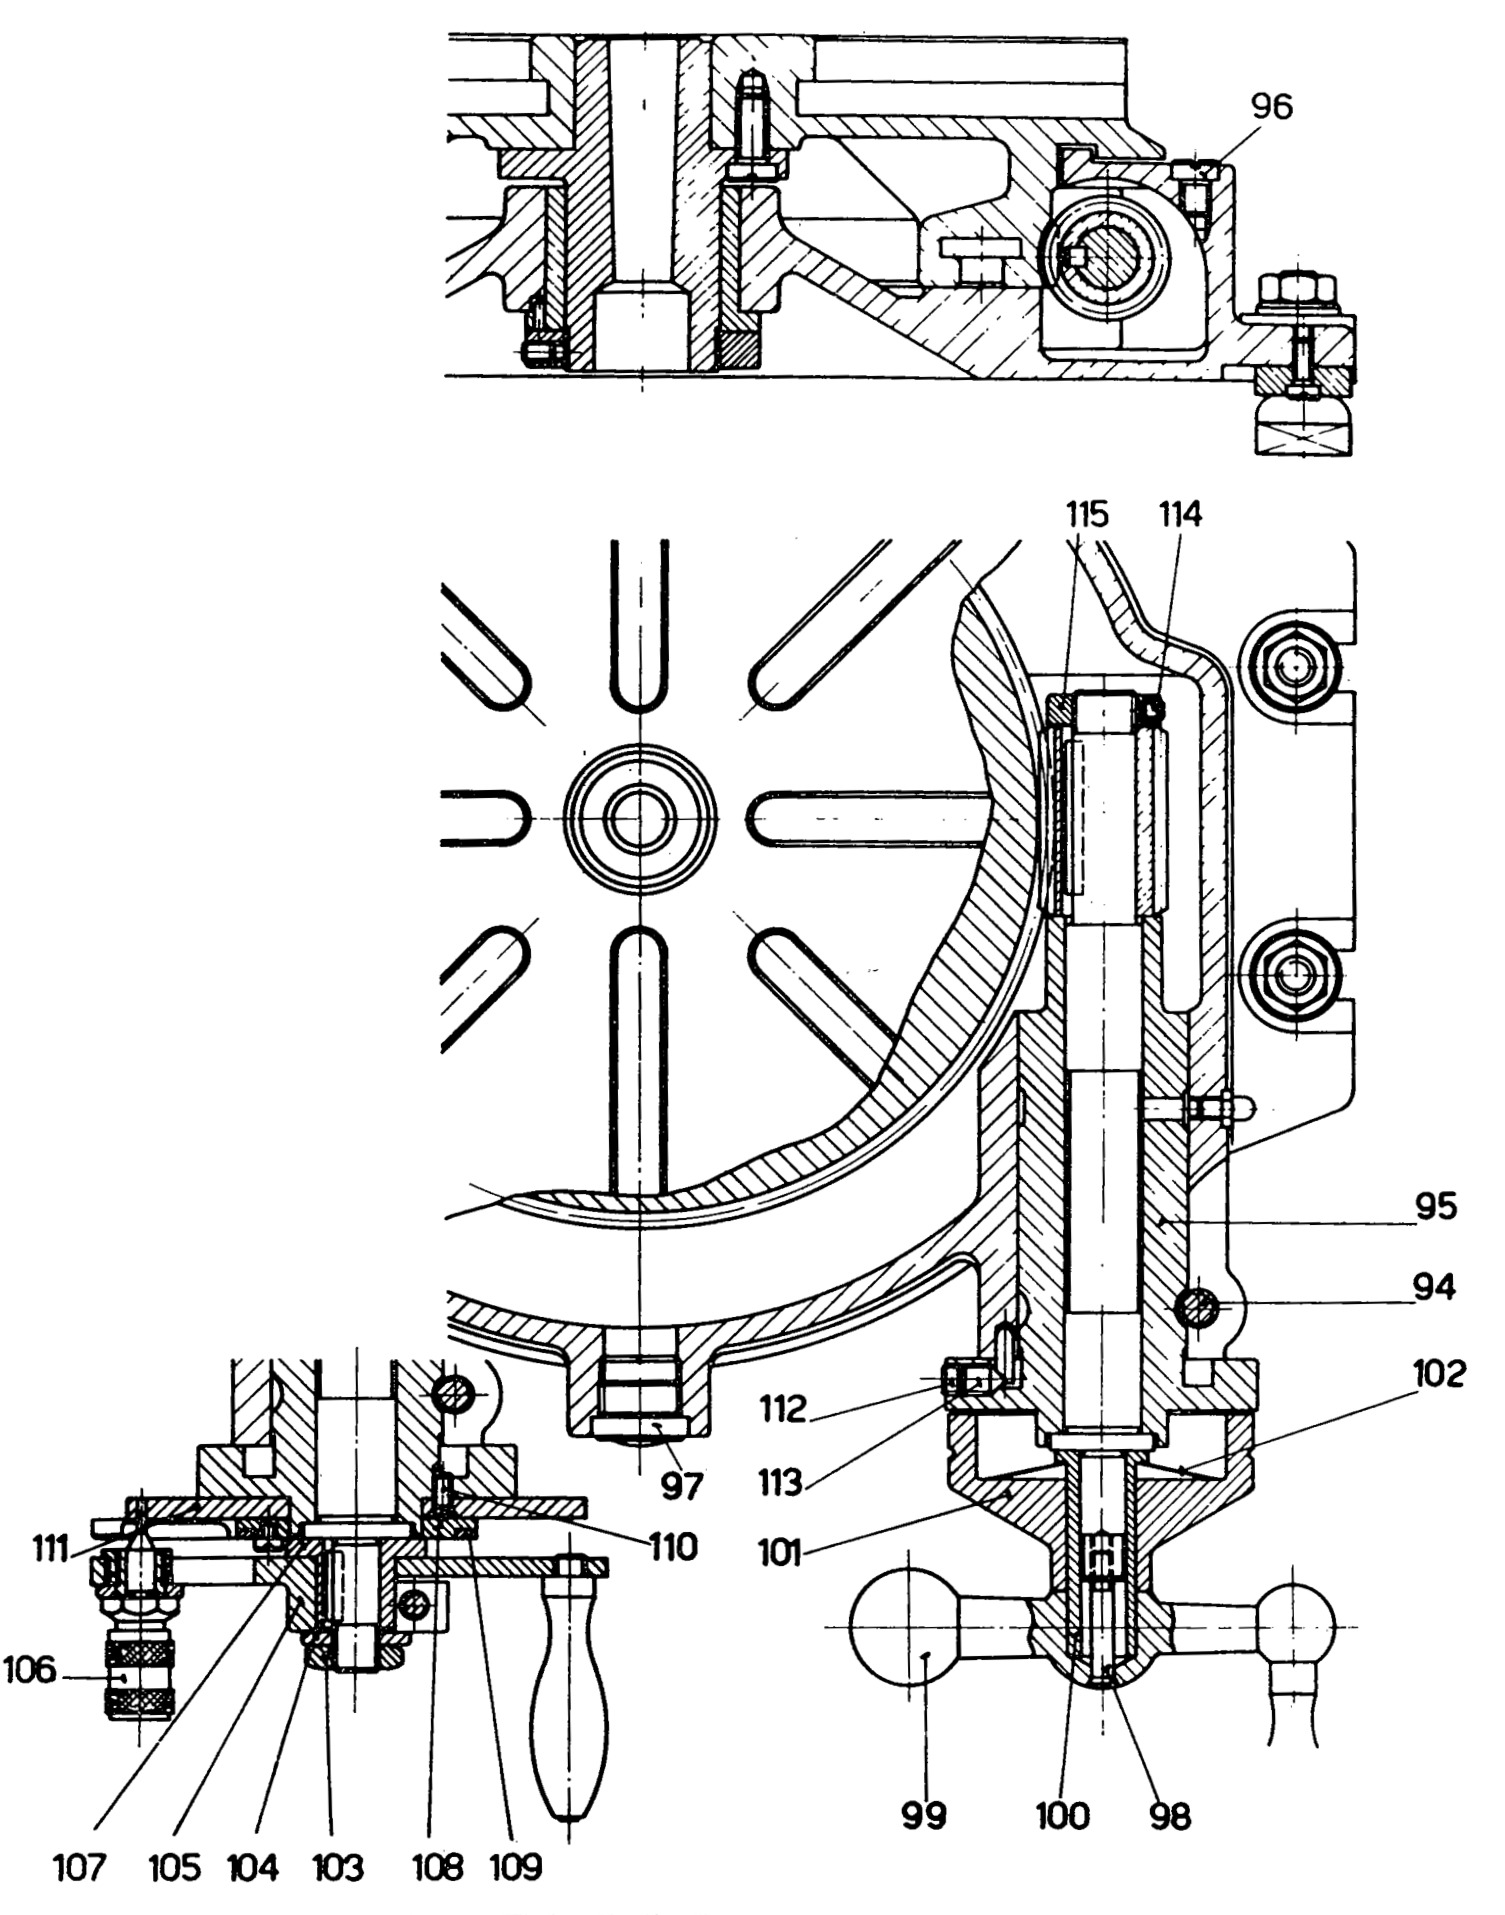
\includegraphics[width=1.0\linewidth]{images/page_33}
    \caption{Example PNG Image}
    \label{fig:rotary_table}
\end{figure}

    \chapter{Vertical Head Service Manual}

\section*{Accessories No. 201, resp. 201A}

\begin{tabular}{ll}
    Internal Taper                               & ISO 30              \\
    Spindle Bore                                 & Ø 15 mm             \\
    Diameter of cutter arbors, long and short    & 13-16-22-25,4-27 mm \\
    Inclination                                  & \(360^\circ\)       \\
    Spindle Speeds (by infinitely-variable gear) & 58 - 2000 rpm       \\
\end{tabular}

\section*{Cleaning, Lubrication, and Maintenance}

Upon receipt and during operation, the general guidelines provided for the machine must be observed.
The vertical head includes 3 oilers for pressure lubrication using the pump supplied with the machine.

\section*{Installation}

The vertical head is centered and secured by the two support arms 7.
For installation, insert the gear stud 141 (supplied with the vertical head) into the spindle nose,
then tighten it using the tightening key. Extend one of the support arms 7 by approximately 250 mm and lock the front screw 5.
Mount the vertical head on the cleared arm, unlock screw 5, and insert the second support arm into the corresponding bore of the vertical head.

This mounting process avoids potential jams during simultaneous engagement of both support arms.
Then, press the vertical head against the spindle head, taking care not to damage the gear teeth.
Secure the support arms 7 with the two screws 5 and tighten screw 142, pressing the vertical head firmly against the spindle head to prevent any torsion.
Finally, lock the two fastening screws that hold the vertical head against the spindle head.

\section*{Spindle Cutter Adjustment}

The bearing adjustment is done during the setup of each vertical head, so a new adjustment is necessary only after a relatively long running time.

The front bearing includes a tapered roller bearing 143 from Precision Industrielle in Rueil-Malmaison (France) No. 101.040 / 101.080 (precision 2 Microns).

The rear bearing includes a tapered roller bearing 144 No. 102.035 / 102.072, of the same origin and precision as the front bearing.

\section*{Compensation of Spindle Axial Play}

\begin{enumerate}
    \item Separate the tiltable part from the fixed part by unscrewing the 4 locking nuts.
    \item Unscrew screw 145 and remove cover 147.
    \item Unscrew nut 148 connected to the spindle 149 by the lock washer 150, lifting one of the tabs engaged in one of the nut entries. Remove baffle 146.
    \item Carefully tap the spindle 149 with a lead hammer.
    \item Plane spacer 152 for half of the play to be compensated, which has been previously determined by precise control.
    \item Plane spacer 153 for half of the play to be compensated.
    \item Reassemble the spindle 149 in the reverse direction of disassembly, remembering to fold down the tab of the washer 150 blocking nut 148 and to lock screw 145.
\end{enumerate}

    \newpage
\begin{figure}[h]
    \centering
    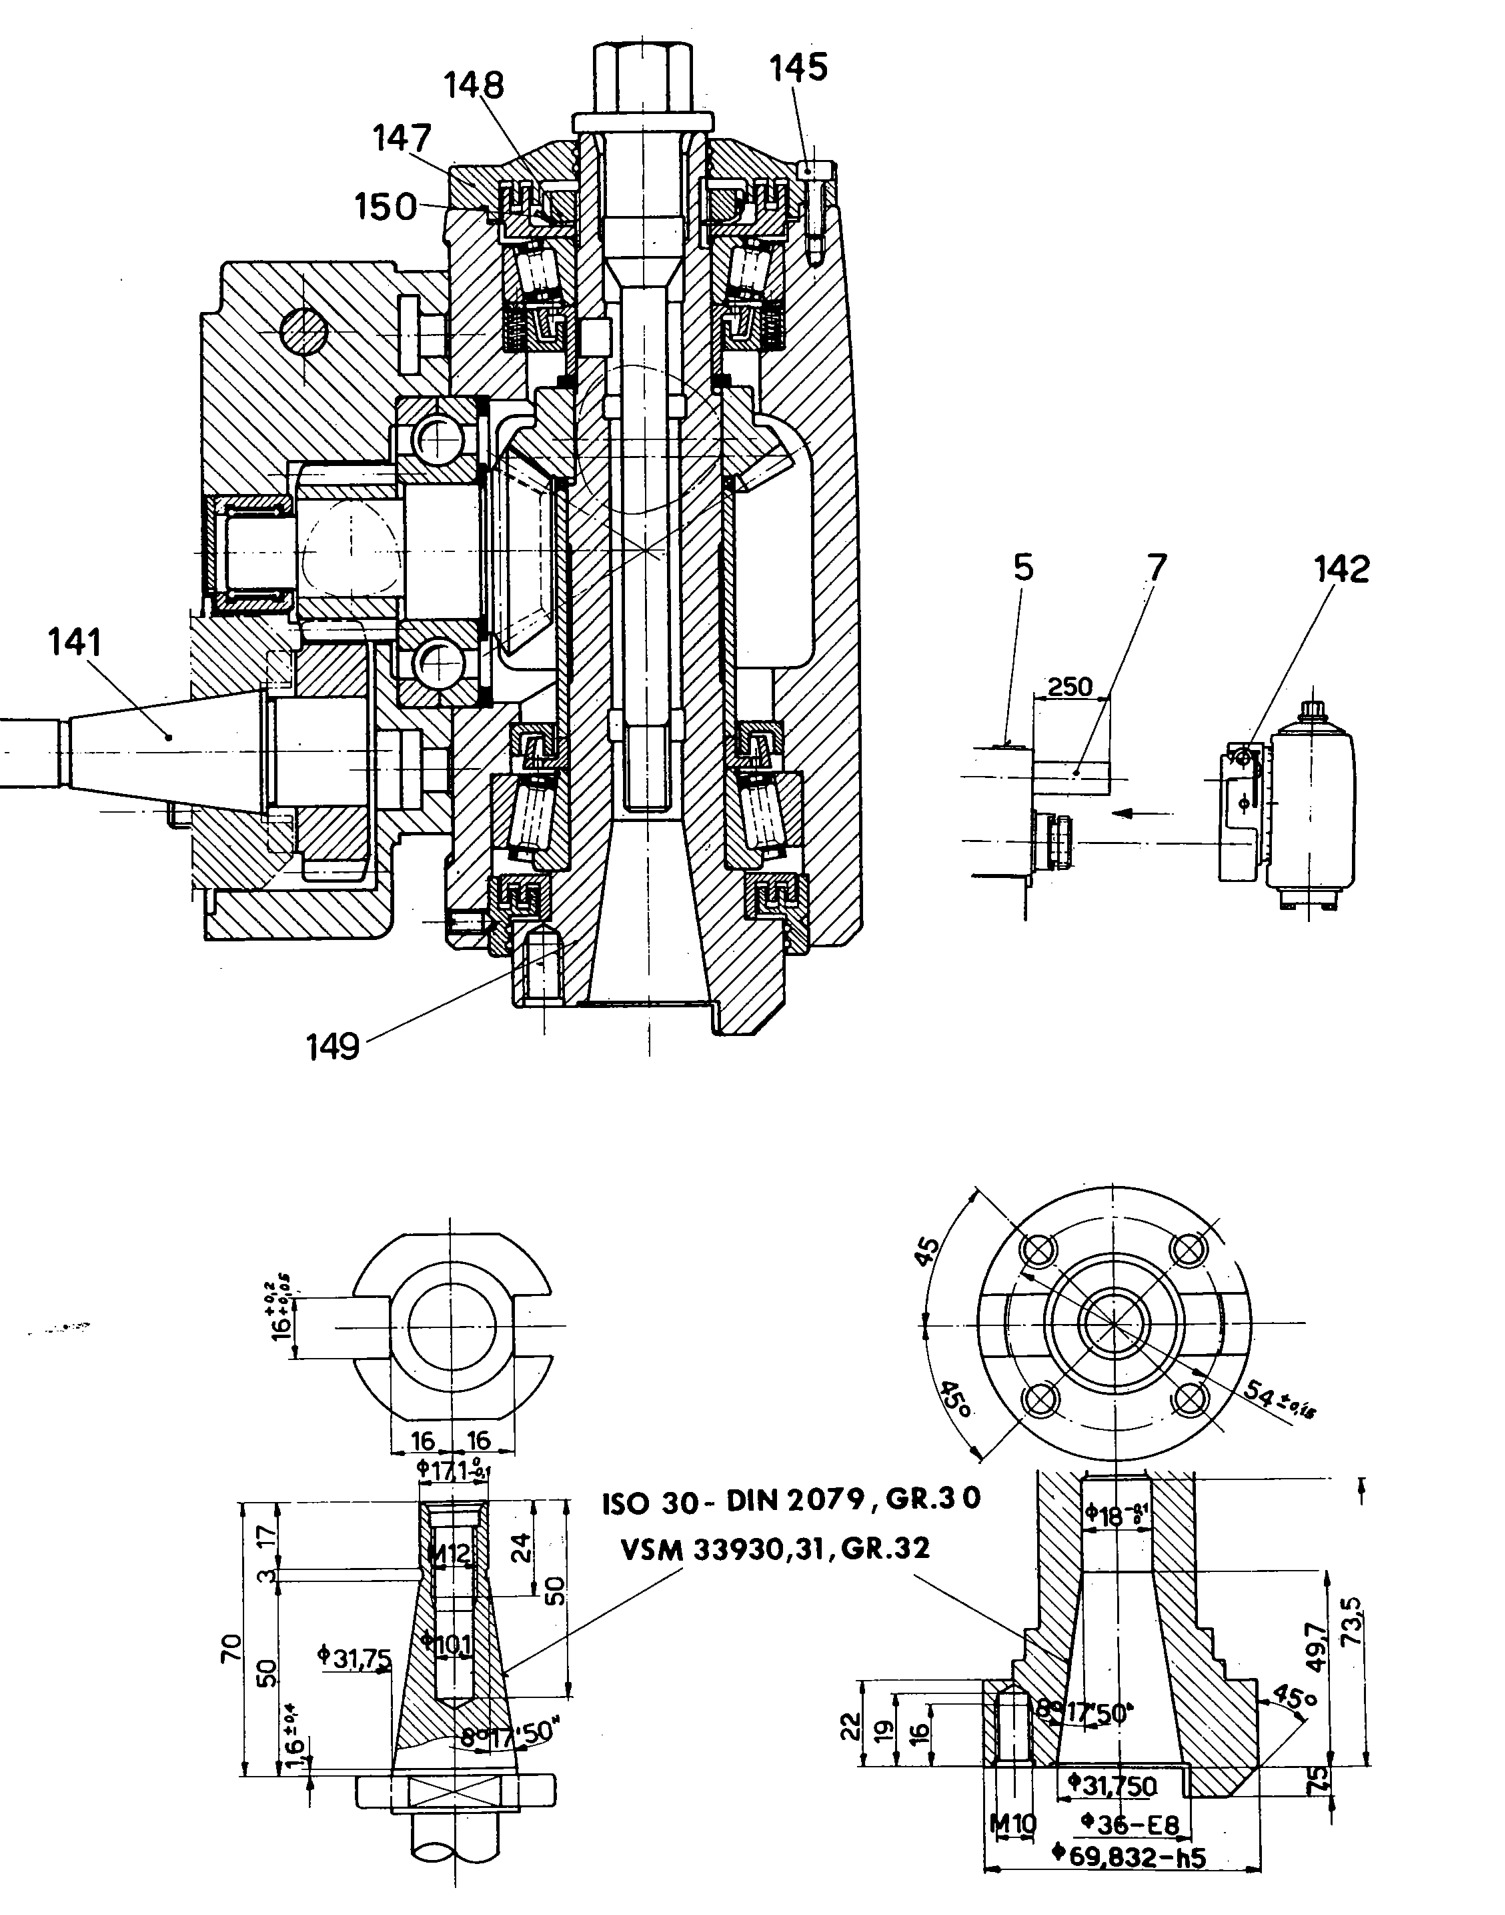
\includegraphics[width=1.0\linewidth]{images/page_35}
    \caption{Example PNG Image}
    \label{fig:milling_head}
\end{figure}

    \newpage
\begin{figure}[h]
    \centering
    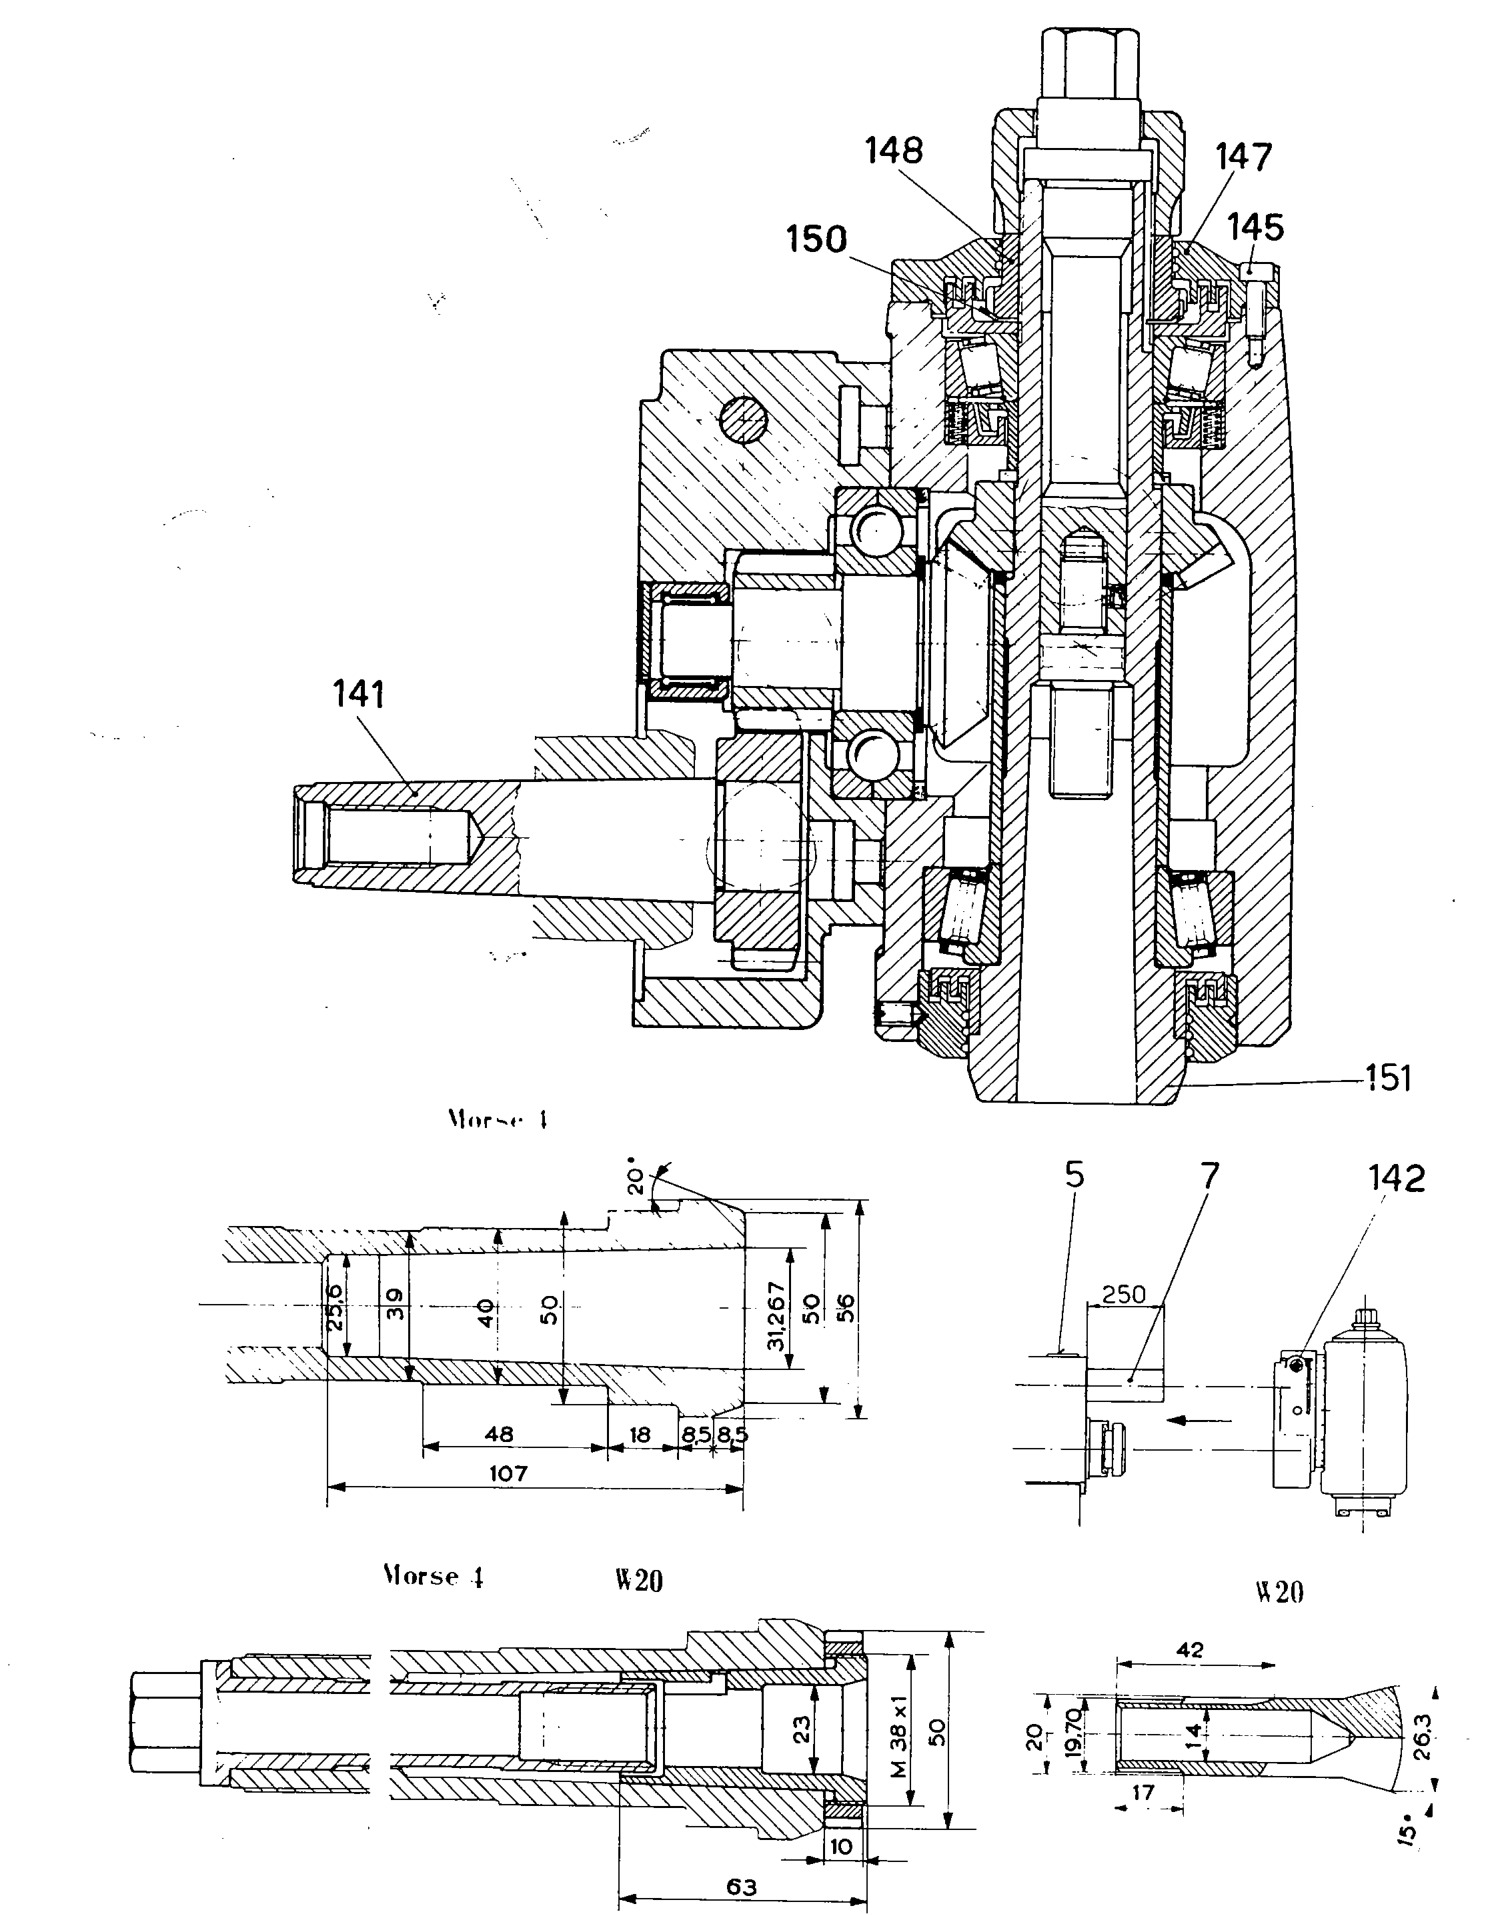
\includegraphics[width=1.0\linewidth]{images/page_36}
    \caption{Example PNG Image}
    \label{fig:milling_head_2}
\end{figure}

    \chapter{Service Instructions for the Mortising Head \\
SCHAUBLIN 13 \small(Accessory No. 1200)}


\section*{Main Features}

\begin{tabular}{@{}ll@{}}
    Adjustable stroke            & 0 to 60 mm      \\
    Number of strokes per minute & 60--430         \\
    Tilt                         & \(\pm90^\circ\) \\
    Chisel dimensions            & 12 x 12 mm      \\
\end{tabular}

\section*{Cleaning, Lubrication, and Maintenance}
Upon receipt and during use, the general instructions provided for the machine must be observed.
The mortising head includes 3 oilers for pressure lubrication using the pump supplied with the machine.

\section*{Installation}
The mortising head is centered and secured by the two support arms (7).
For installation, insert the gear rack (154) provided with the mortising head into the spindle nose, then tighten it using the tightening key.
Extend one of the support arms (7) by approximately 250 mm, lock the front screw (5), mount the mortising head on the freed arm, unlock the screw (5), and insert the second support arm into the corresponding bore of the mortising head.

This mounting procedure avoids jamming that may occur during the simultaneous engagement of both support arms.
Press the mortising head against the face of the spindle head, taking care not to damage the gear teeth.
Secure the support arms (7) using the two screws (5) and tighten the screw (80) by pressing the mortising head firmly against the spindle head to prevent any torsion.
Finally, lock the two fixing screws (81).

The number of strokes must be limited to 430, which corresponds to a spindle speed of 405 rpm.

\begin{figure}[h]
    \centering
    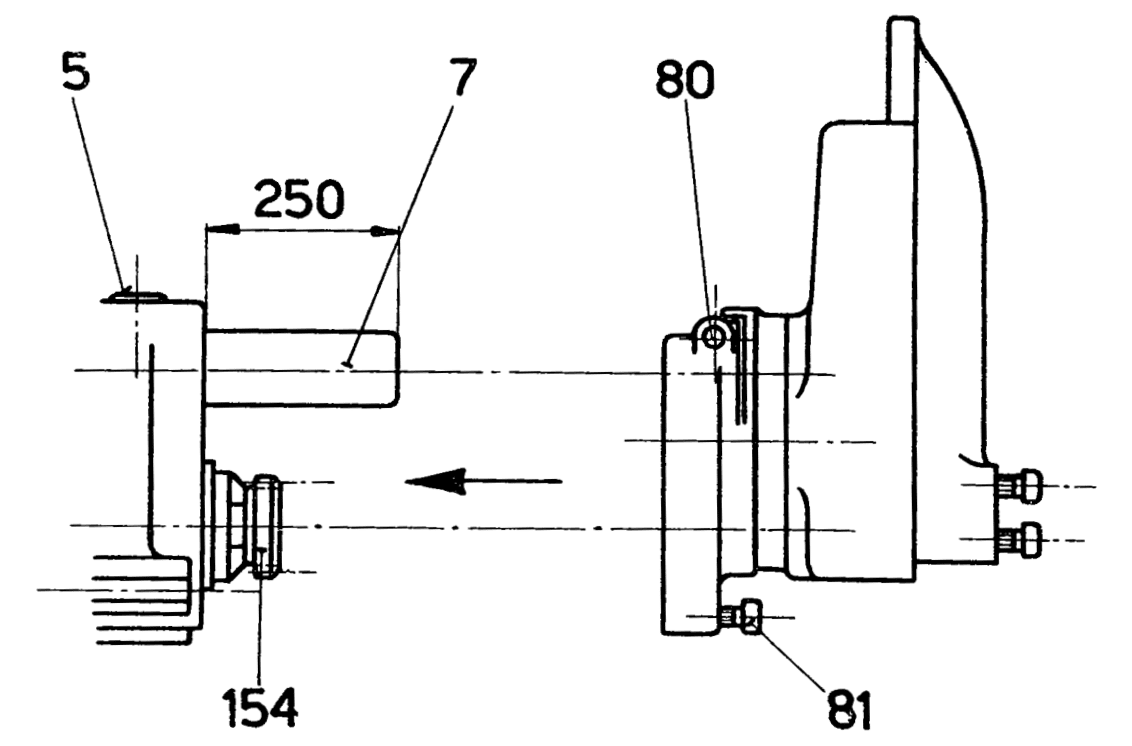
\includegraphics[width=0.7\linewidth]{images/page_37}
    \caption{Mortising Head Installation}
    \label{fig:mortising_head_installation}
\end{figure}

    \newpage

\section*{Adjusting the Slide Stroke}

\begin{enumerate}
    \item Position screw 87 in front of the adjustment opening for accessibility with the key.
    \item Loosen nut 88. (Turn only half a turn as indicated on the plate!)
    \item Adjust the stroke using screw 87. This adjustment is facilitated by ruler 89 following index 90.
    \item Lock screw 88. (Important!)
\end{enumerate}

\section*{Adjusting the Chisel Tilt}

The chisel is secured by two screws 99.

\begin{enumerate}
    \item Loosen both screws 92.
    \item Set the desired tilt of the chisel holder 93 using screws 94.
    \item Lock both screws 92.
\end{enumerate}

\section*{Adjusting the Conical Gib 95}

The adjustment is simply done using screw 96.

    \newpage
\begin{figure}[h]
    \centering
    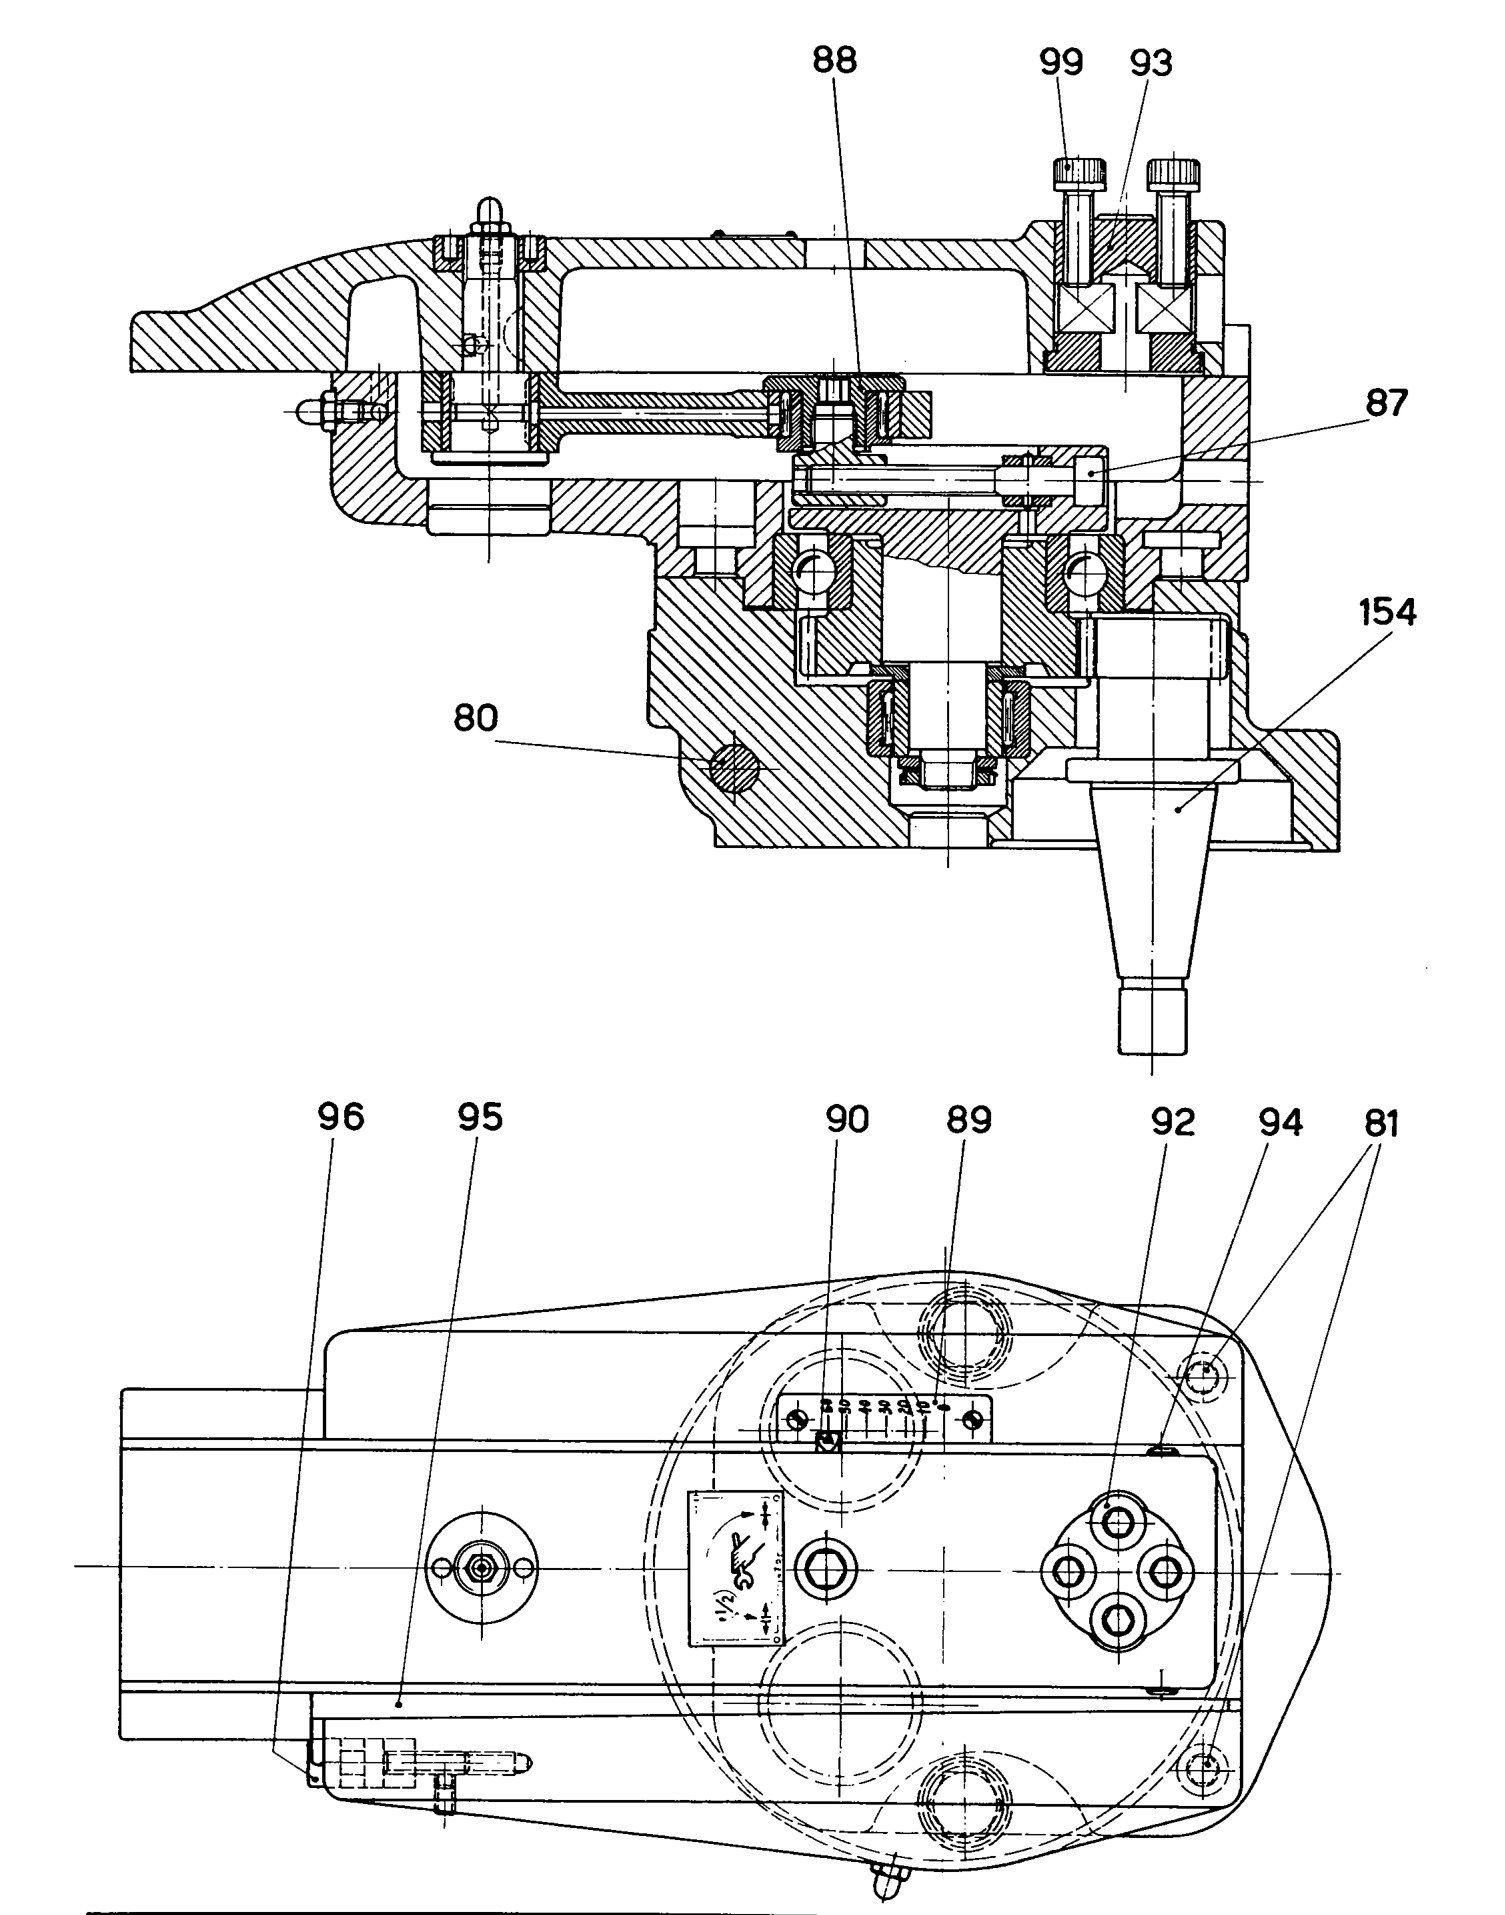
\includegraphics[width=1.0\linewidth]{images/page_39}
    \caption{Mortising Head}
    \label{fig:mortising_head}
\end{figure}

    \chapter{Service Instructions for the High Speed Head \\
SCHAUBLIN 13 \small{Accessory No. 1100}}

\section*{Main Features}
\begin{tabular}{@{}ll@{}}
    Inner spindle cone for E20 collet & E20            \\
    Spindle stroke                    & 60 mm          \\
    Spindle speed (3 x normal speeds) & 170 - 6400 rpm \\
    Spindle tilt                      & 360°           \\
\end{tabular}

\section*{Accessories}
\begin{tabular}{@{}lp{0.7\linewidth}@{}}
    437E & Biconical collet E20 with concentric clamping. Bore diameters from Ø 3 to 10 mm.                                                                                           \\
    1184 & Dial indicator with mounting bracket for depth measurement. 1 division = 0.0025 mm.                                                                                        \\
    235B & Boring chuck Ø 24 mm for bores from 2 to 40 mm. Cylindrical shank Ø 10 mm. Key, reduction sleeves, square, tool holder, high-speed steel tools, and shims in a wooden box. \\
\end{tabular}

\section*{Cleaning, Lubrication, and Maintenance}
Upon receipt and during use, follow the general guidelines provided for the machine. The quick head includes 2 oilers for pressurized lubrication using the pump supplied with the machine.

\section*{Installation}
The quick head is centered and secured by the two support arms 7. For installation, insert the gear rack 141 (supplied with the quick head and identical to that of the vertical head) into the spindle nose, then tighten it with the wrench. Extend one of the support arms 7 by about 250 mm and lock the front screw 5. Mount the quick head on the support arm in the corresponding bore of the quick head. This mounting method avoids jams that may occur when both support arms engage simultaneously. Then press the quick head against the face of the spindle head, taking care not to damage the gear teeth. Immobilize the support arms 7 with the two screws 5 and tighten the locking screw 80 by pressing the quick head firmly against the spindle head to prevent any torsion. Finally, tighten the 2 fixing screws 81.

\section*{Spindle}

The front bearing consists of a double-row ball bearing 120 (SKF 3205-C153) specially designed for high speeds. The rear bearing is a ball bearing 121 (SKF 6205-C153). If either of these bearings shows excessive wear, replace it as follows:
\vspace{-\parskip}
\begin{enumerate}
    \item To release the spiral spring 119, move the spindle to the upper position; unscrew the 4 fixing screws of the cover 118 and remove the control shaft complete with gear 123 and cover 118.
    \item Remove the cover 124 fixed by 2 screws.
    \item Unscrew the nut 126 locked by the lock washer 127 and remove the gear wheel 128.
    \item Loosen the screw 129 and remove the quill 130 from its housing.
    \item Unscrew the nut 131 locked by the lock washer 132.
    \item Disassemble the spindle 134 and replace the defective bearing.
\end{enumerate}

    \newpage
\begin{figure}[h]
    \centering
    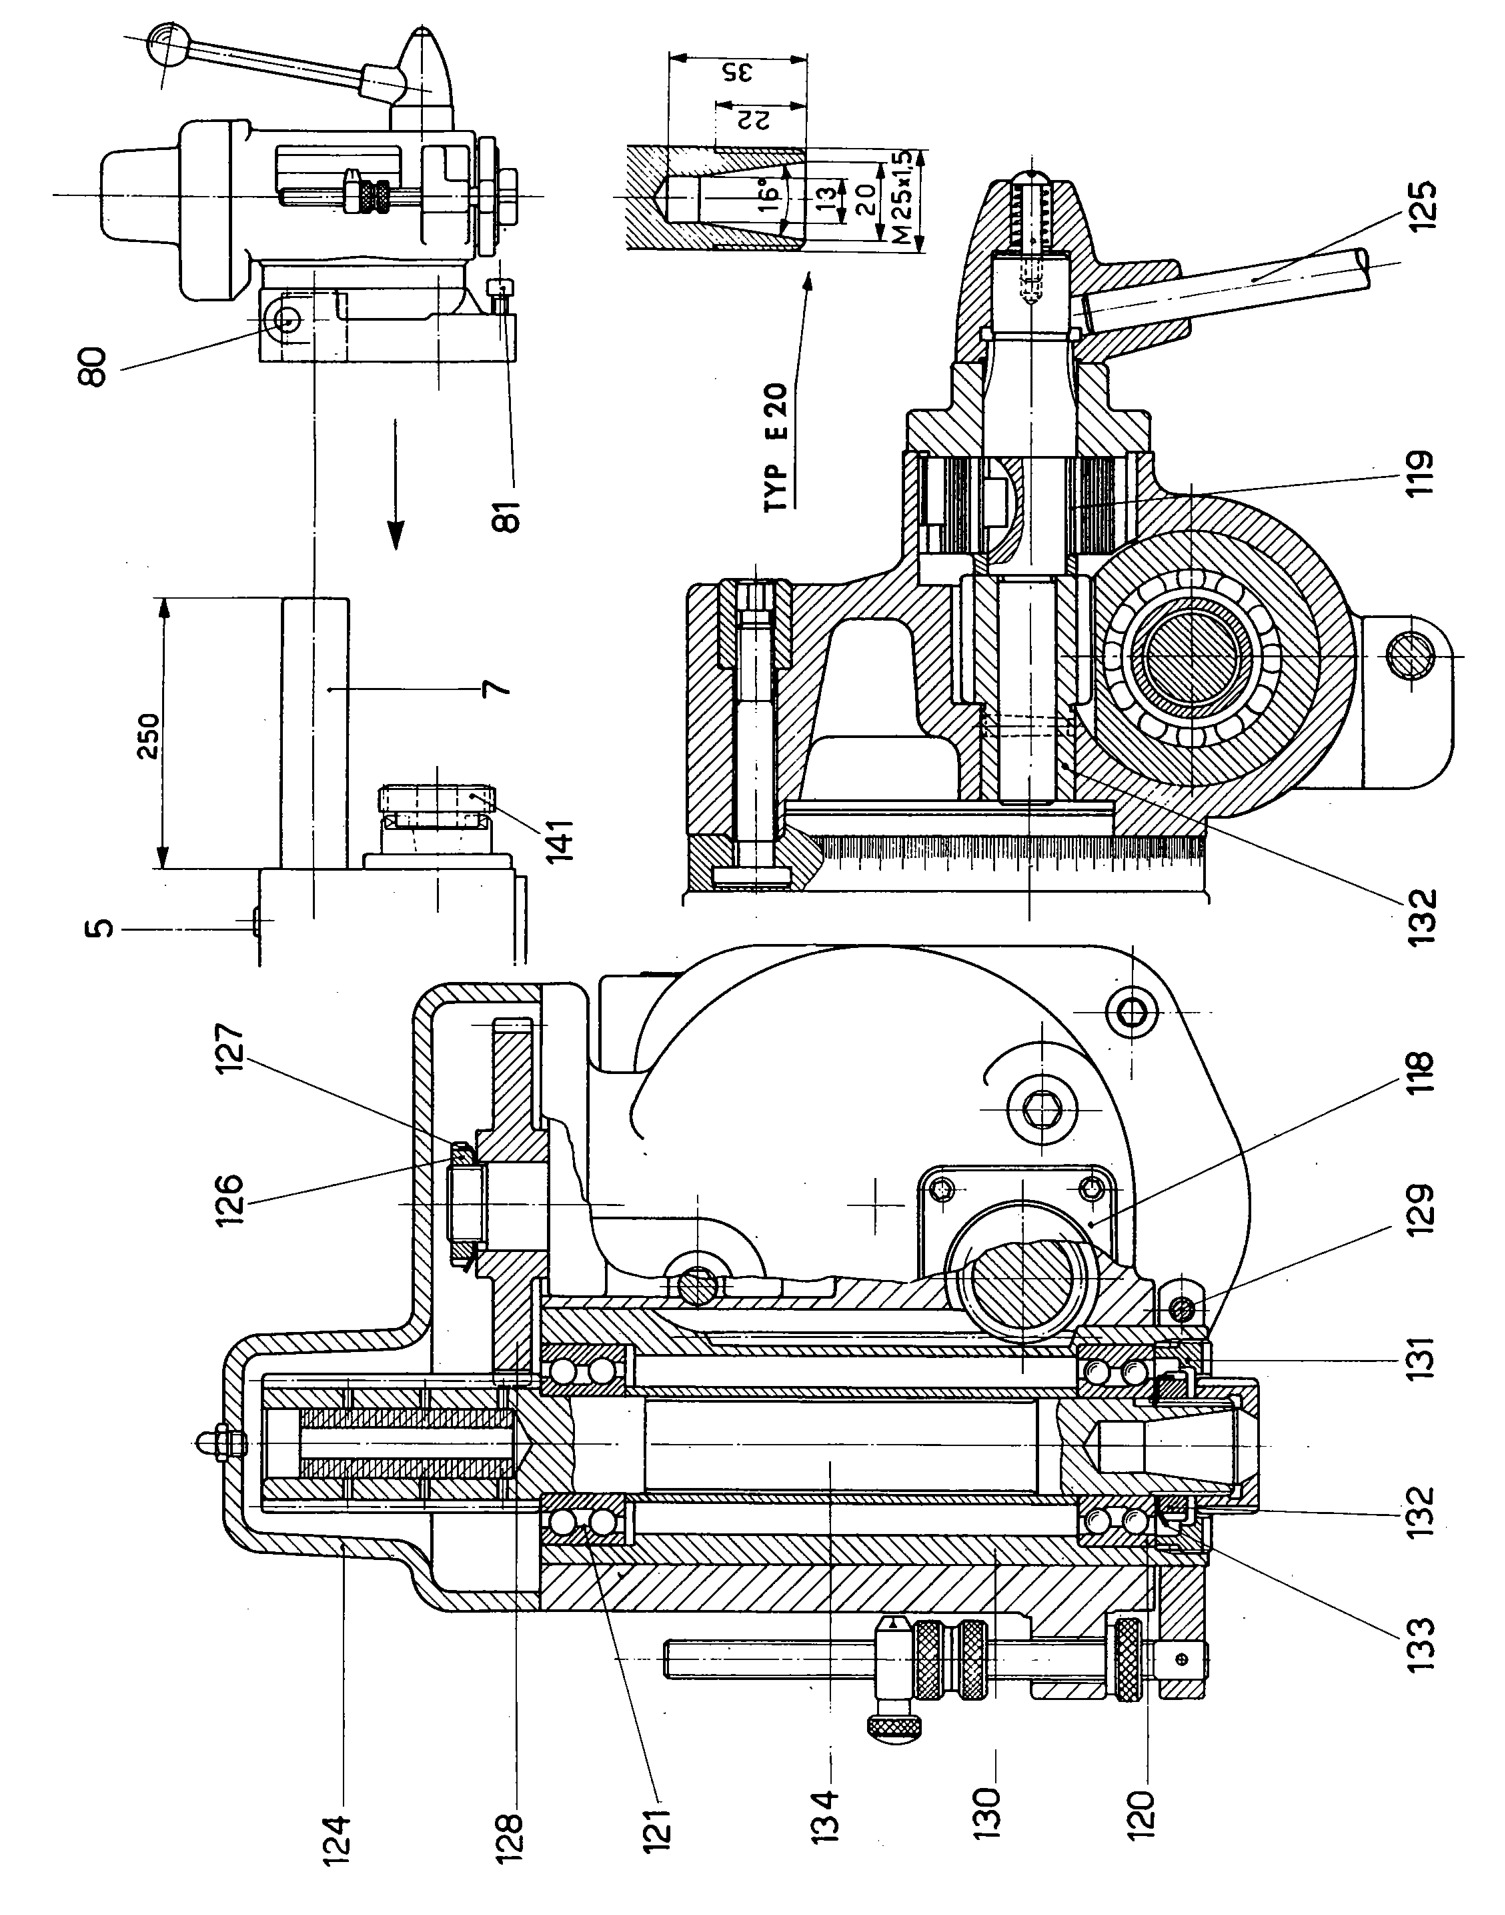
\includegraphics[width=1.0\linewidth]{images/page_41}
    \caption{High Speed Head}
    \label{fig:high_speed_head}
\end{figure}

    \chapter{Service Instructions for Vise 35 For Use on Universal Milling Machine Schaublin 13 \small{Accessory No. 35}}

\section*{Main Features}


\begin{tabular}{@{}ll@{}}
    Jaw Width                        & 100 mm        \\
    Jaw Height                       & 30 mm         \\
    Maximum Opening                  & 70 mm         \\
    Total Height with Swivel Base    & 100 mm        \\
    Total Height without Swivel Base & 75 mm         \\
    Swiveling                        & \(360^\circ\)
\end{tabular}

\section*{Cleaning, Lubrication, and Maintenance}

Upon receipt and during operation, the provided instructions for the machine are valid and must be observed.
The vise includes an oiler for lubrication using a dropper.
By flipping the vise, the screw is accessible for periodic lubrication.

\section*{Usage}

The base is fixed on one of the T-slots of the table using two rods. Two locator blocks ensure alignment.

The vise is secured on the base in all positions by two rods.
Additionally, a central rod presses the base and vise onto the table.
Its effective tightening is at the tool contact point.

For simple tasks, the vise is used without the base.
The locator blocks of the base can be screwed onto the vise body in two positions: parallel or perpendicular to the jaws.
The vise is then fixed on one of the T-slots of the table using the two rods from the base and a shorter central rod,
supplied with this accessory. The effective tightening of the central rod should not be neglected.

    \chapter{Service Instructions for Vise SEL 36 For Use on Universal Milling Machine 13 \small{Accessory No. 36}}

\section*{Main Features}

\begin{tabular}{@{}ll@{}}
    Jaw Width       & 85 mm         \\
    Maximum Opening & 60 mm         \\
    Jaw Height      & 37 mm         \\
    Swiveling       & \(360^\circ\) \\
    Inclination     & \(360^\circ\) \\
    Stop every      & \(15^\circ\)  \\
\end{tabular}

\section*{Cleaning, Lubrication, and Maintenance}

Upon receipt and during operation, follow the provided instructions for the machine, which are valid and must be observed.
The vise includes an oiler for lubrication using a pump.
The horizontal position at \(0^\circ\) (closed jaws) allows lubrication of the sliding jaw and the screw; the vertical position at \(90^\circ\) (jaws on the oiler side) allows lubrication of the guide.

\section*{Usage}

The base is fixed on one of the T-slots of the table using two rods. Two locator blocks ensure alignment.

The vise is locked in all positions in the horizontal plane by two rods.
Inclination can be done throughout the circumference, degree by degree.
However, the exact position is ensured every \(15^\circ\) by a hardened piston.
Locking is done using a keyed nut delivered with the vise.

Good milling results are obtained by following the procedure indicated in the sketch below:

\begin{figure}[h]
    \centering
    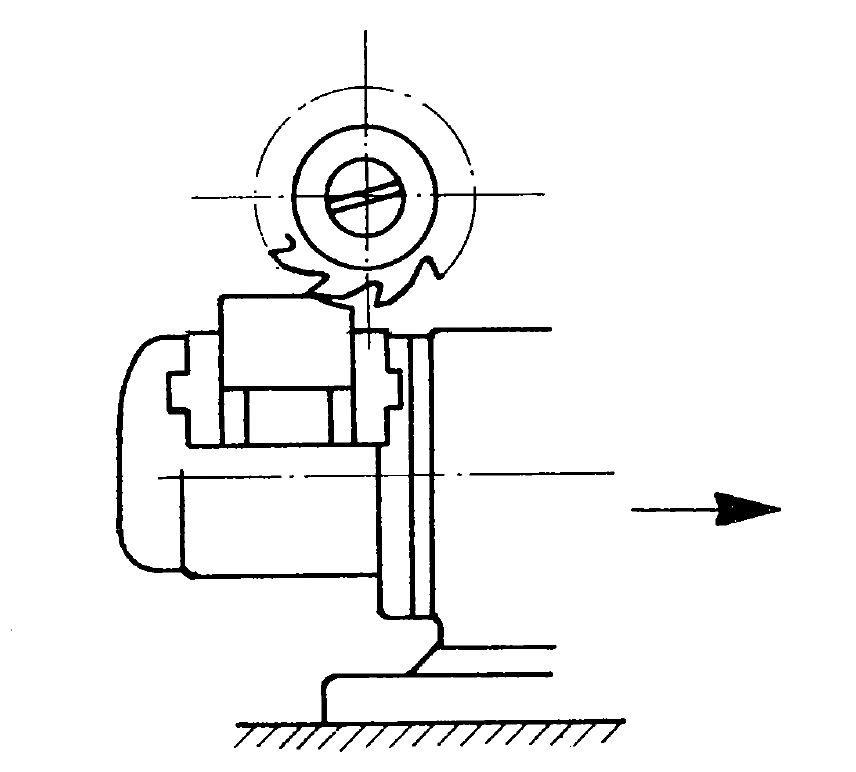
\includegraphics[width=0.5\linewidth]{images/page_43}
    \caption{Milling direction}
    \label{fig:milling_direction}
\end{figure}

    \chapter{Dividing Head \small{Accessory No. 17}}

\section*{Main Features}

\begin{tabular}{@{}ll@{}}
    Center height                        & 62 mm  \\
    Spindle with threaded nose for chuck & No. 21 \\
    Collet bore                          & W20    \\
    Solid center with tightening key     &        \\
    Bench profile base                   &
\end{tabular}

\section*{Accessories}
\begin{tabular}{@{}ll@{}}
    780  & Long support arm, length 375 mm                            \\
    781  & Long support arm, length 475 mm                            \\
    110  & Circular divider, 60 teeth                                 \\
    108  & Spring ratchet                                             \\
    82   & 4-disc hole divider device                                 \\
    83   & Vernier dividing device                                    \\
    9012 & Drive dog                                                  \\
    4    & Clamp Type W20 Collet, Max Bore 20 mm, Max Passage 14.5 mm \\
\end{tabular}

\section*{Cleaning, Lubrication, and Maintenance}
Upon receipt and during operation, follow the provided instructions for the machine, which are valid and must be observed.
The dividing head includes an oiler for pressure lubrication using the pump supplied with the machine.

\section*{Installation}
The dividing head and the tailstock are fixed using tie rods on the swivel base No. 50 with a bench profile of 102.
This base allows a center distance of 265 mm.
For between-center work on base No. 8001, use arms No. 780 or 781, providing center distances of 105 or 205 mm.

The spindle is locked using lever 100.

\section*{Compensation of Spindle Axial Play}
\begin{enumerate}
    \item Unlock screws 101.
    \item Screw nut 102 according to the amount of play to be compensated.
    \item Tighten firmly both screws 101.
\end{enumerate}

\section*{Vernier Disassembly}
\begin{enumerate}
    \item Unscrew screw 103.
    \item Remove the pinion 104, the sleeve 105 carrying the vernier 106.
\end{enumerate}

\section*{Disassembly of Hole Disks}
\begin{enumerate}
    \item Unscrew screw 107.
    \item Remove the crank 108, the washer 109, and the needles 110.
    \item Unscrew the 3 screws 111 and remove disk 112.
\end{enumerate}

To release the spindle from the worm, unlock screw 113 and turn support 114.

    \newpage
\begin{figure}[h]
    \centering
    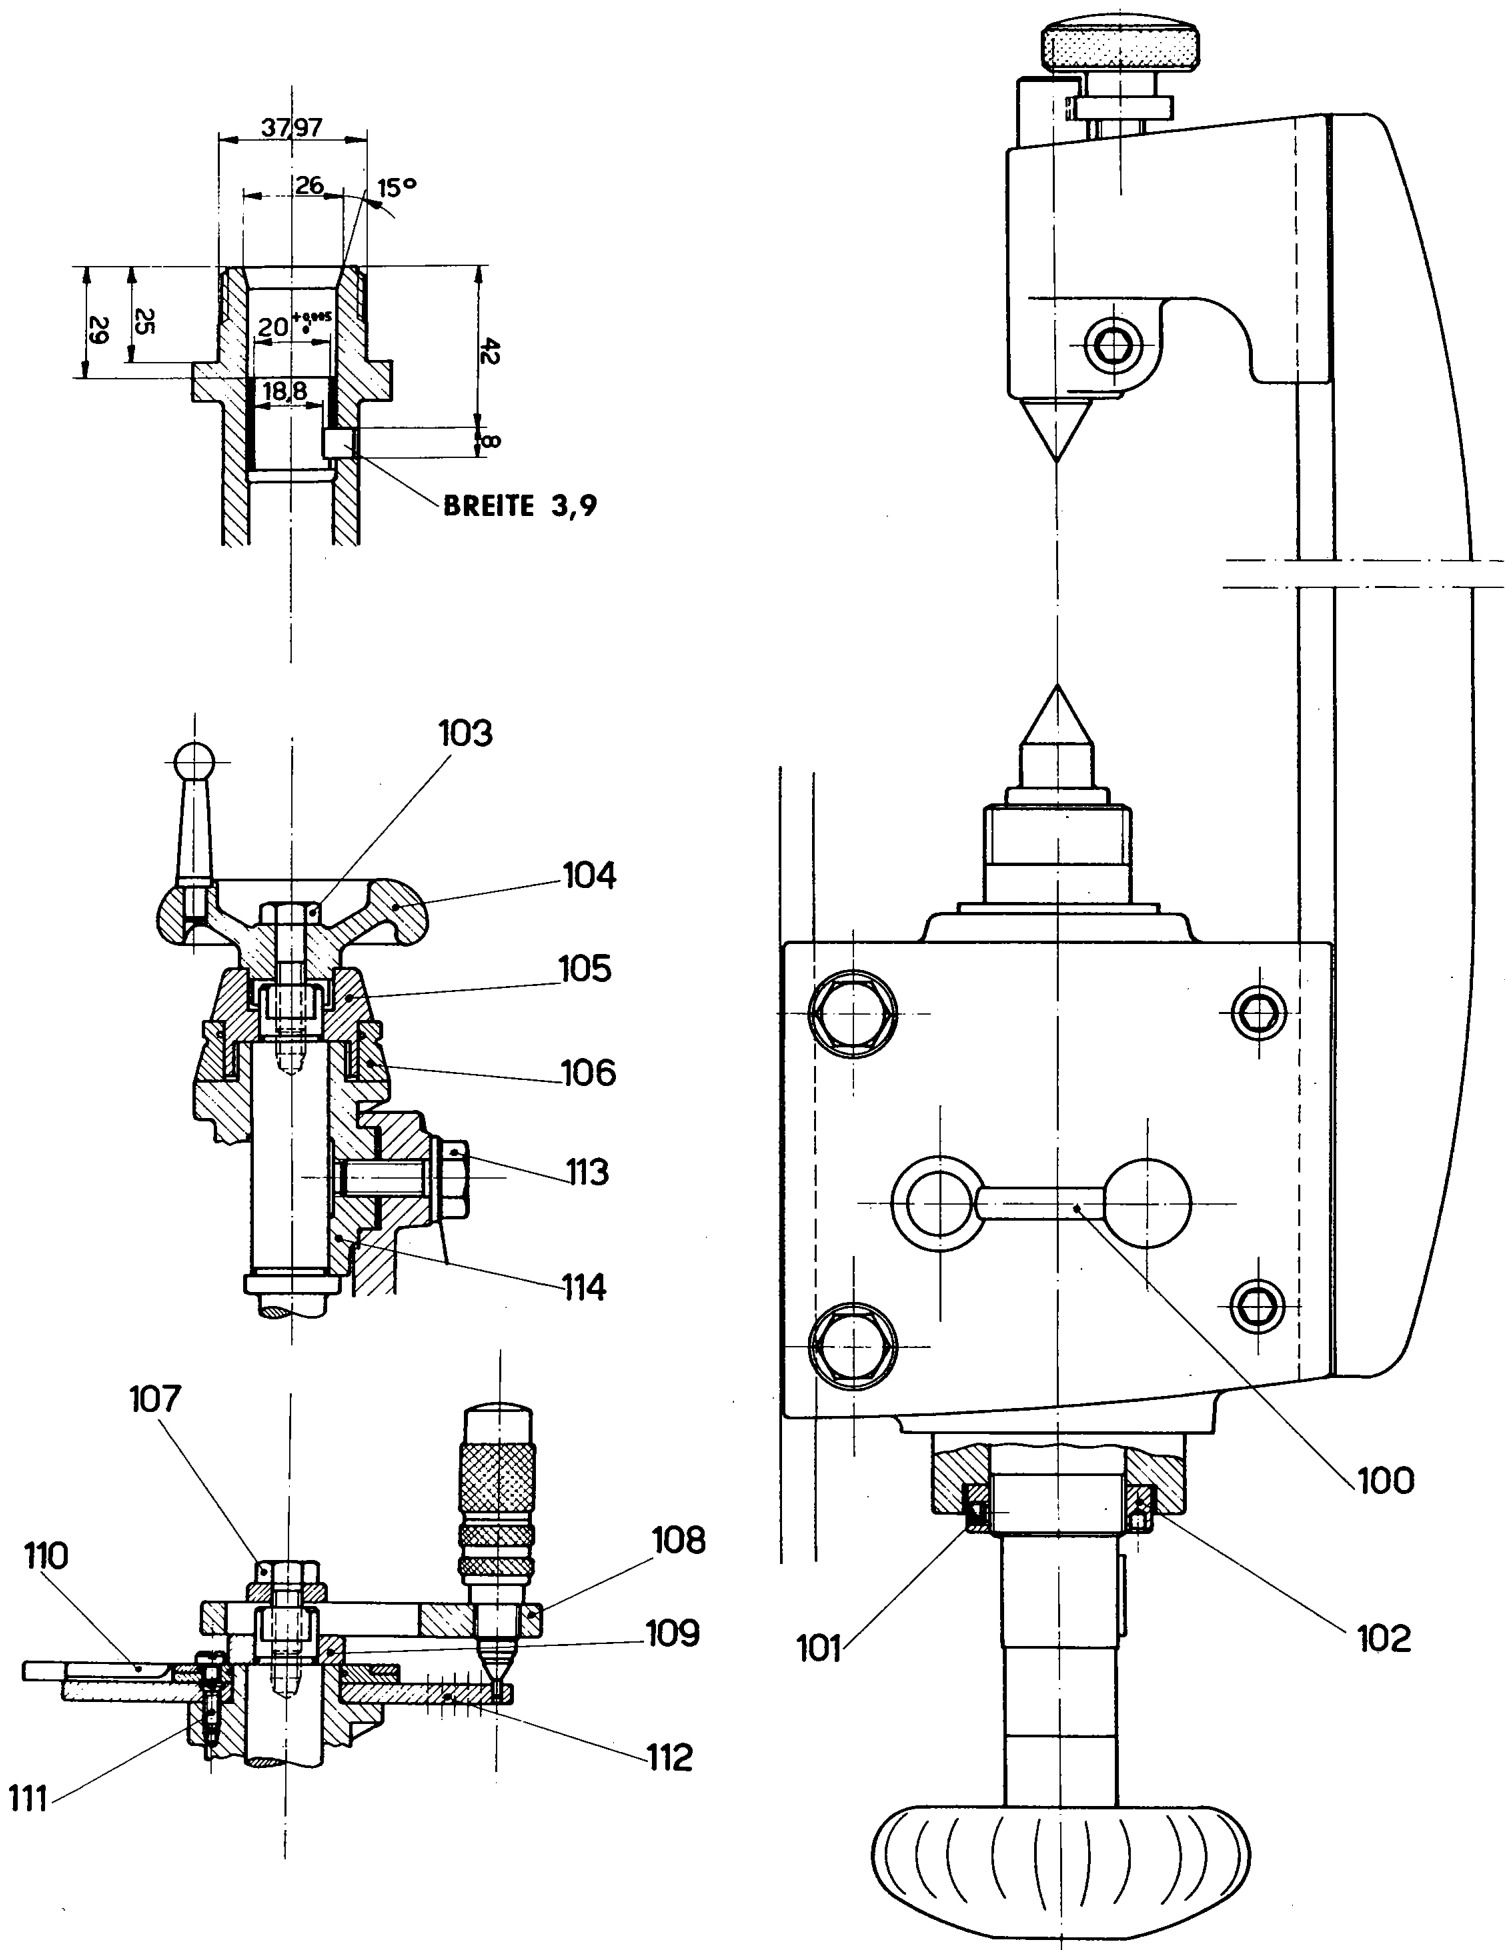
\includegraphics[width=1.0\linewidth]{./images/page_45}
    \caption{Dividing Head}
    \label{fig:dividing_head}
\end{figure}

    \chapter{Service Instructions for Dividing Head \small{Accessory No. 12/17 + 12/102}}

\section*{Main Features}
\begin{tabular}{@{}ll@{}}
    Center height:                                               & As per specification \\
    Spindle with threaded nose like dividing head W20 for chuck: & Yes                  \\
    Collet bore:                                                 & As per specification \\
    Bench profile base:                                          & 102                  \\
\end{tabular}

\section*{Accessories}
\begin{tabular}{@{}ll@{}}
    110        & Circular divider, 60 teeth                          \\
    108        & Spring ratchet                                      \\
    82         & 4-disc hole divider device                          \\
    102-20.064 & Chuck with 2 sets of 3 jaws, adjusted on the plate  \\
    85         & Drive plate Ø 100 mm, with pin                      \\
    4          & W20 Collets, max bore 20 mm, passage beyond 14.5 mm \\
    616        & Quick clamping by lever
\end{tabular}

\section*{Cleaning, Lubrication, and Maintenance}
Upon receipt and during operation, follow the provided instructions for the machine, which must be observed.

The dividing head spindle quill has a hole 103 for lubricating the spindle.
Periodically remove the quill from the quill holder by loosening the 2 screws to oil. The hole 103 should be at the top.

\section*{Compensation of Spindle Axial Play}
\begin{enumerate}
    \item Unlock the 2 screws 104.
    \item Screw nut 105 while controlling the axial play with the comparator. It should be 0.008 mm.
    \item Tighten firmly the 2 screws 104.
\end{enumerate}

\section*{Disassembly of Hole Disks}
\begin{enumerate}
    \item Unscrew nut 106.
    \item Remove washer 107, crank 108.
    \item Remove the spring ring 109 and withdraw the needles 110.
    \item Unscrew the 3 screws 111 and remove disk 112.
\end{enumerate}

To release the spindle from the worm, unlock screw 113 and turn support 114.

    \newpage
\begin{figure}[h]
    \centering
    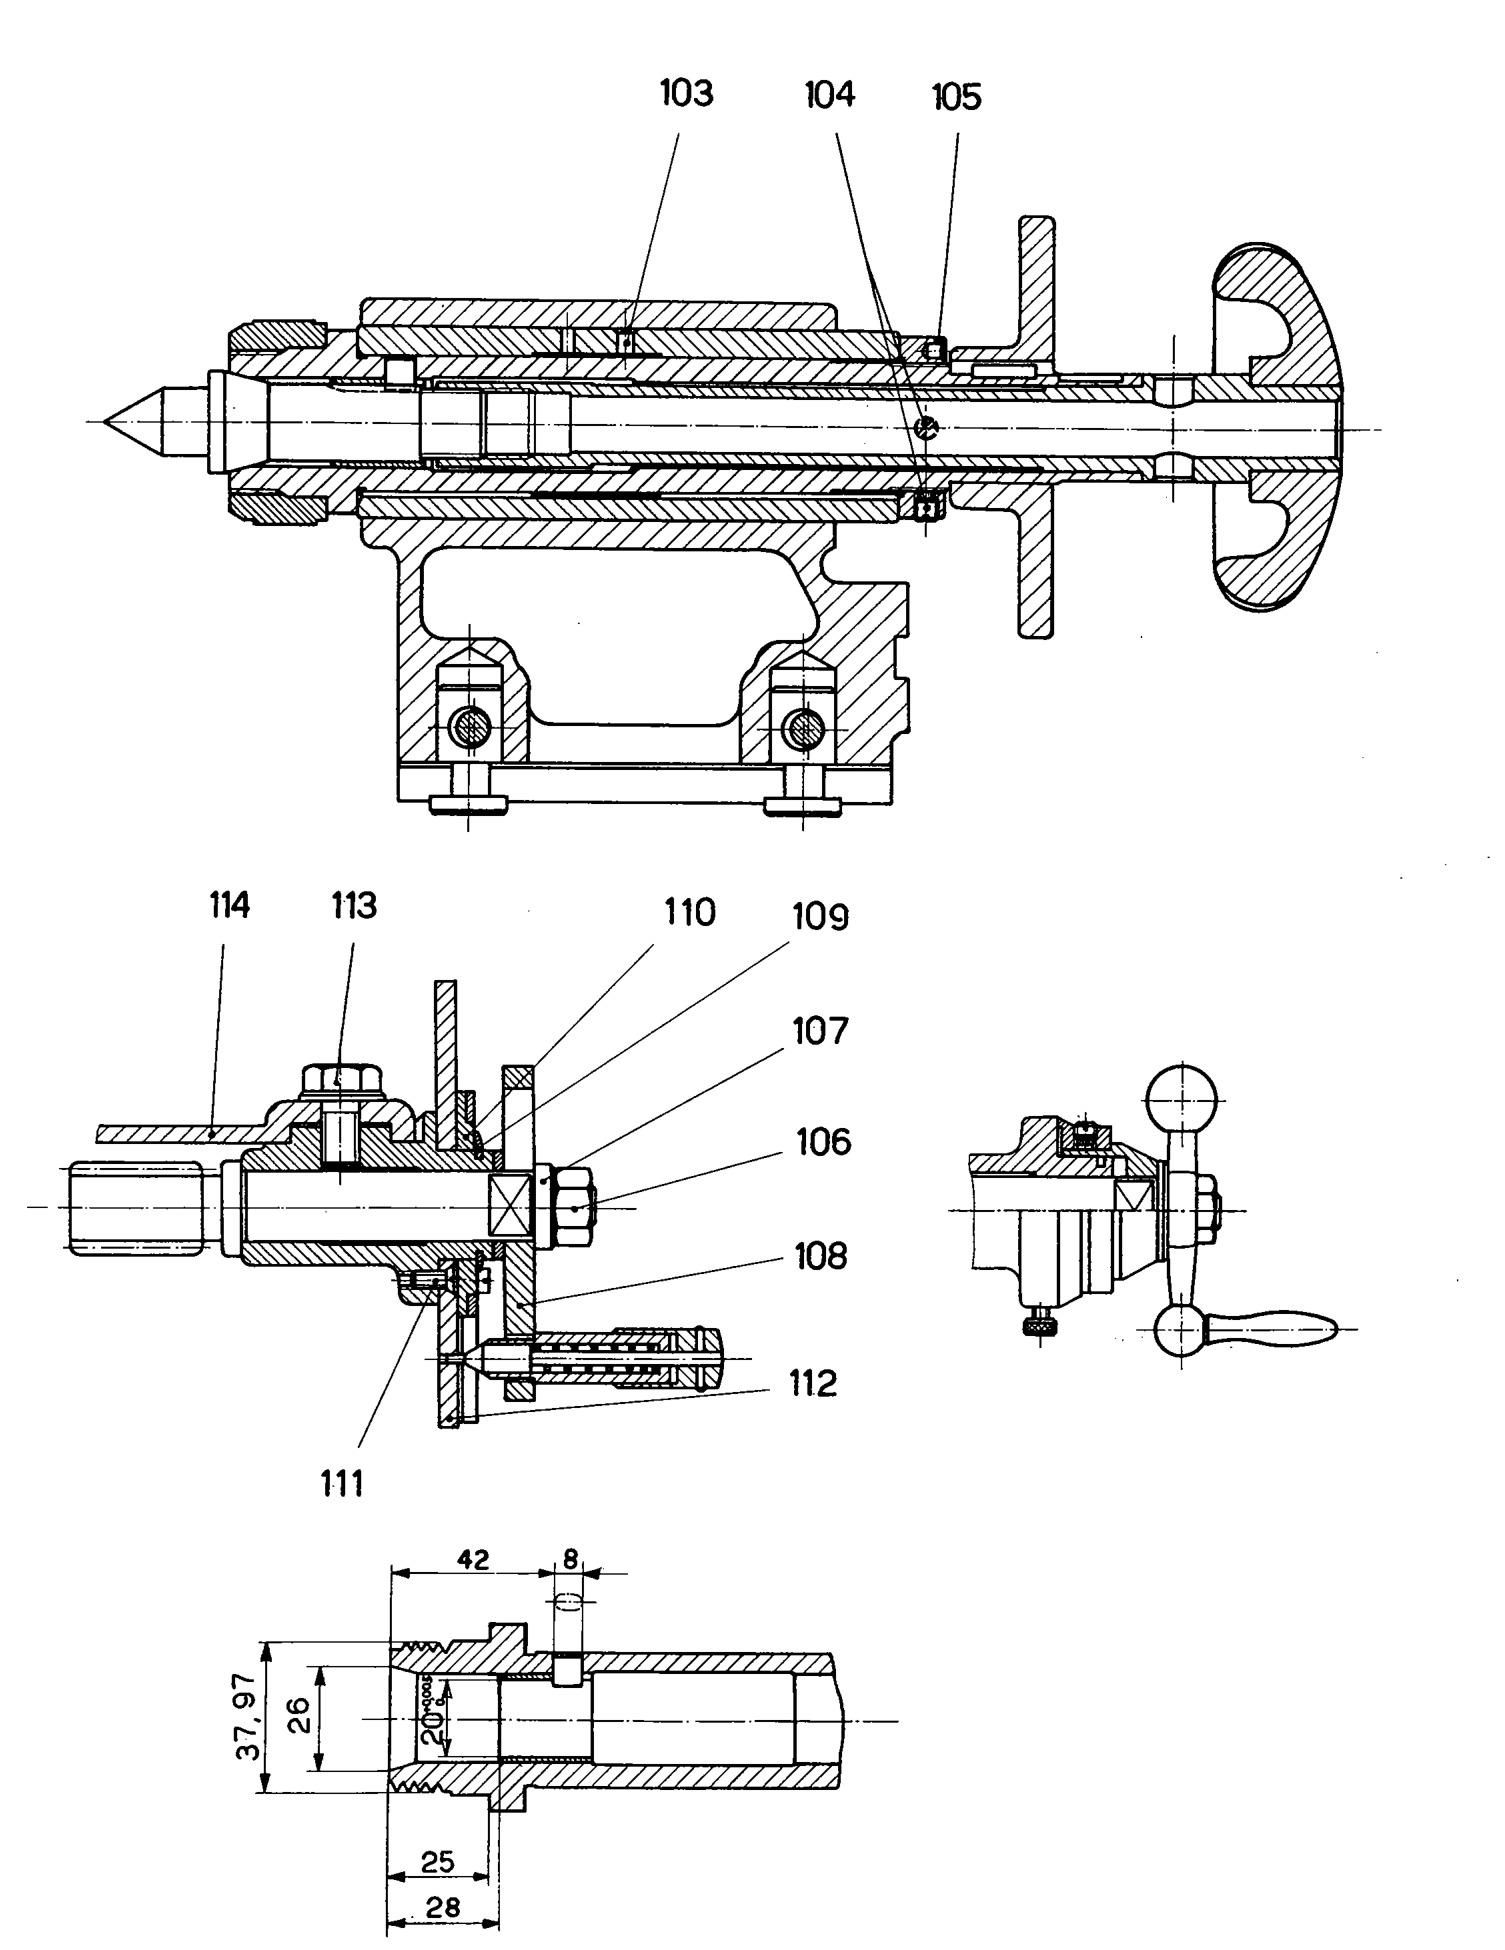
\includegraphics[width=1.0\linewidth]{./images/page_47}
    \caption{Dividing Head}
    \label{fig:dividing_head_2}
\end{figure}

    \chapter{Service Instructions for Universal Dividing Head \small{Accessory No. 900}}

\section*{Main Features}
\begin{tabular}{@{}ll@{}}
    Center height                        & 105 mm        \\
    Rotation                             & \(360^\circ\) \\
    Spindle with threaded nose for chuck & Yes           \\
    Solid center and drive dog           & Yes           \\
    24-hole disk and 3 hole disks        & Yes           \\
\end{tabular}

\section*{Accessories}
\begin{tabular}{@{}ll@{}}
    No 940B    & Automatic control in connection with table feed, including headstock with set of gears, all mounted in a protective casing. \\
    1000       & Tailstock with solid center, Morse spindle taper 0.                                                                         \\
    102-20.064 & Chuck Ø 102 mm with 2 sets of 3 concentric jaws, adjusted on the plate.                                                     \\
    994        & Extension for using the dividing head with automatic control in the middle of the table.                                    \\
    4          & Set of W20 collets. Max bore 20 mm, passage beyond max 14.5 mm.                                                             \\
\end{tabular}

\section*{Cleaning, Lubrication, and Maintenance}
Upon receipt and during operation, follow the provided instructions for the machine, which must be observed.
The universal dividing head includes 5 oilers for pressure lubrication using the pump supplied with the machine.

\section*{Installation and Use}
The dividing head is fixed on the machine table using the two tie rods supplied with this accessory.
The dividing head allows the execution of simple division processes, as well as the cutting of helices and cams.
All these operations are facilitated by the use of the division tables in the attached 13D instruction.

    \section*{Compensation of Spindle Play}

The two spindle bearings consist of high-precision tapered roller bearings, 155 and 156.

\begin{table}[h]
    \centering
    \begin{tabular}{@{}lll@{}}
        \textbf{Bearing Type} & \textbf{Manufacturer}                              & \textbf{Precision}             \\
        \hline
        Front Bearing         & La Précision Industrielle, Rueil-Malmaison, France & N° 101.040/101.080 (2 Microns) \\
        Rear Bearing          & La Précision Industrielle, Rueil-Malmaison, France & N° 100.035/100.072 (2 Microns) \\
    \end{tabular}
\end{table}

These bearings are protected by sealing joints.

\subsection*{Compensation of Spindle Play Procedure}
\begin{enumerate}
    \item Unlock screw 157 and disengage the worm.
    \item Unscrew nut 158.
    \item Remove disk 159, seal 160, ring 161, and key 162.
    \item Take out the inner ring of bearing 156.
    \item Unscrew screw 163 and remove gear 164.
    \item Unscrew the 3 screws 165 and remove the cage 166 containing the outer ring of bearing 156.
    \item Unscrew locking screw 167 and remove the worm wheel 168, along with its key 169.
    \item Take out the spacer 170 and plane it according to the play to be compensated, previously determined by precise control.
    \item Reassemble following the reverse order of disassembly.
\end{enumerate}

\subsection*{Compensation of Worm Play Procedure}
\begin{enumerate}
    \item Unlock screw 157.
    \item Unlock screw 171.
    \item Unscrew piston 172 according to the amount of play to be compensated.
    \item Lock screws 171 and then 157.
\end{enumerate}

    \newpage
\begin{figure}[h]
    \centering
    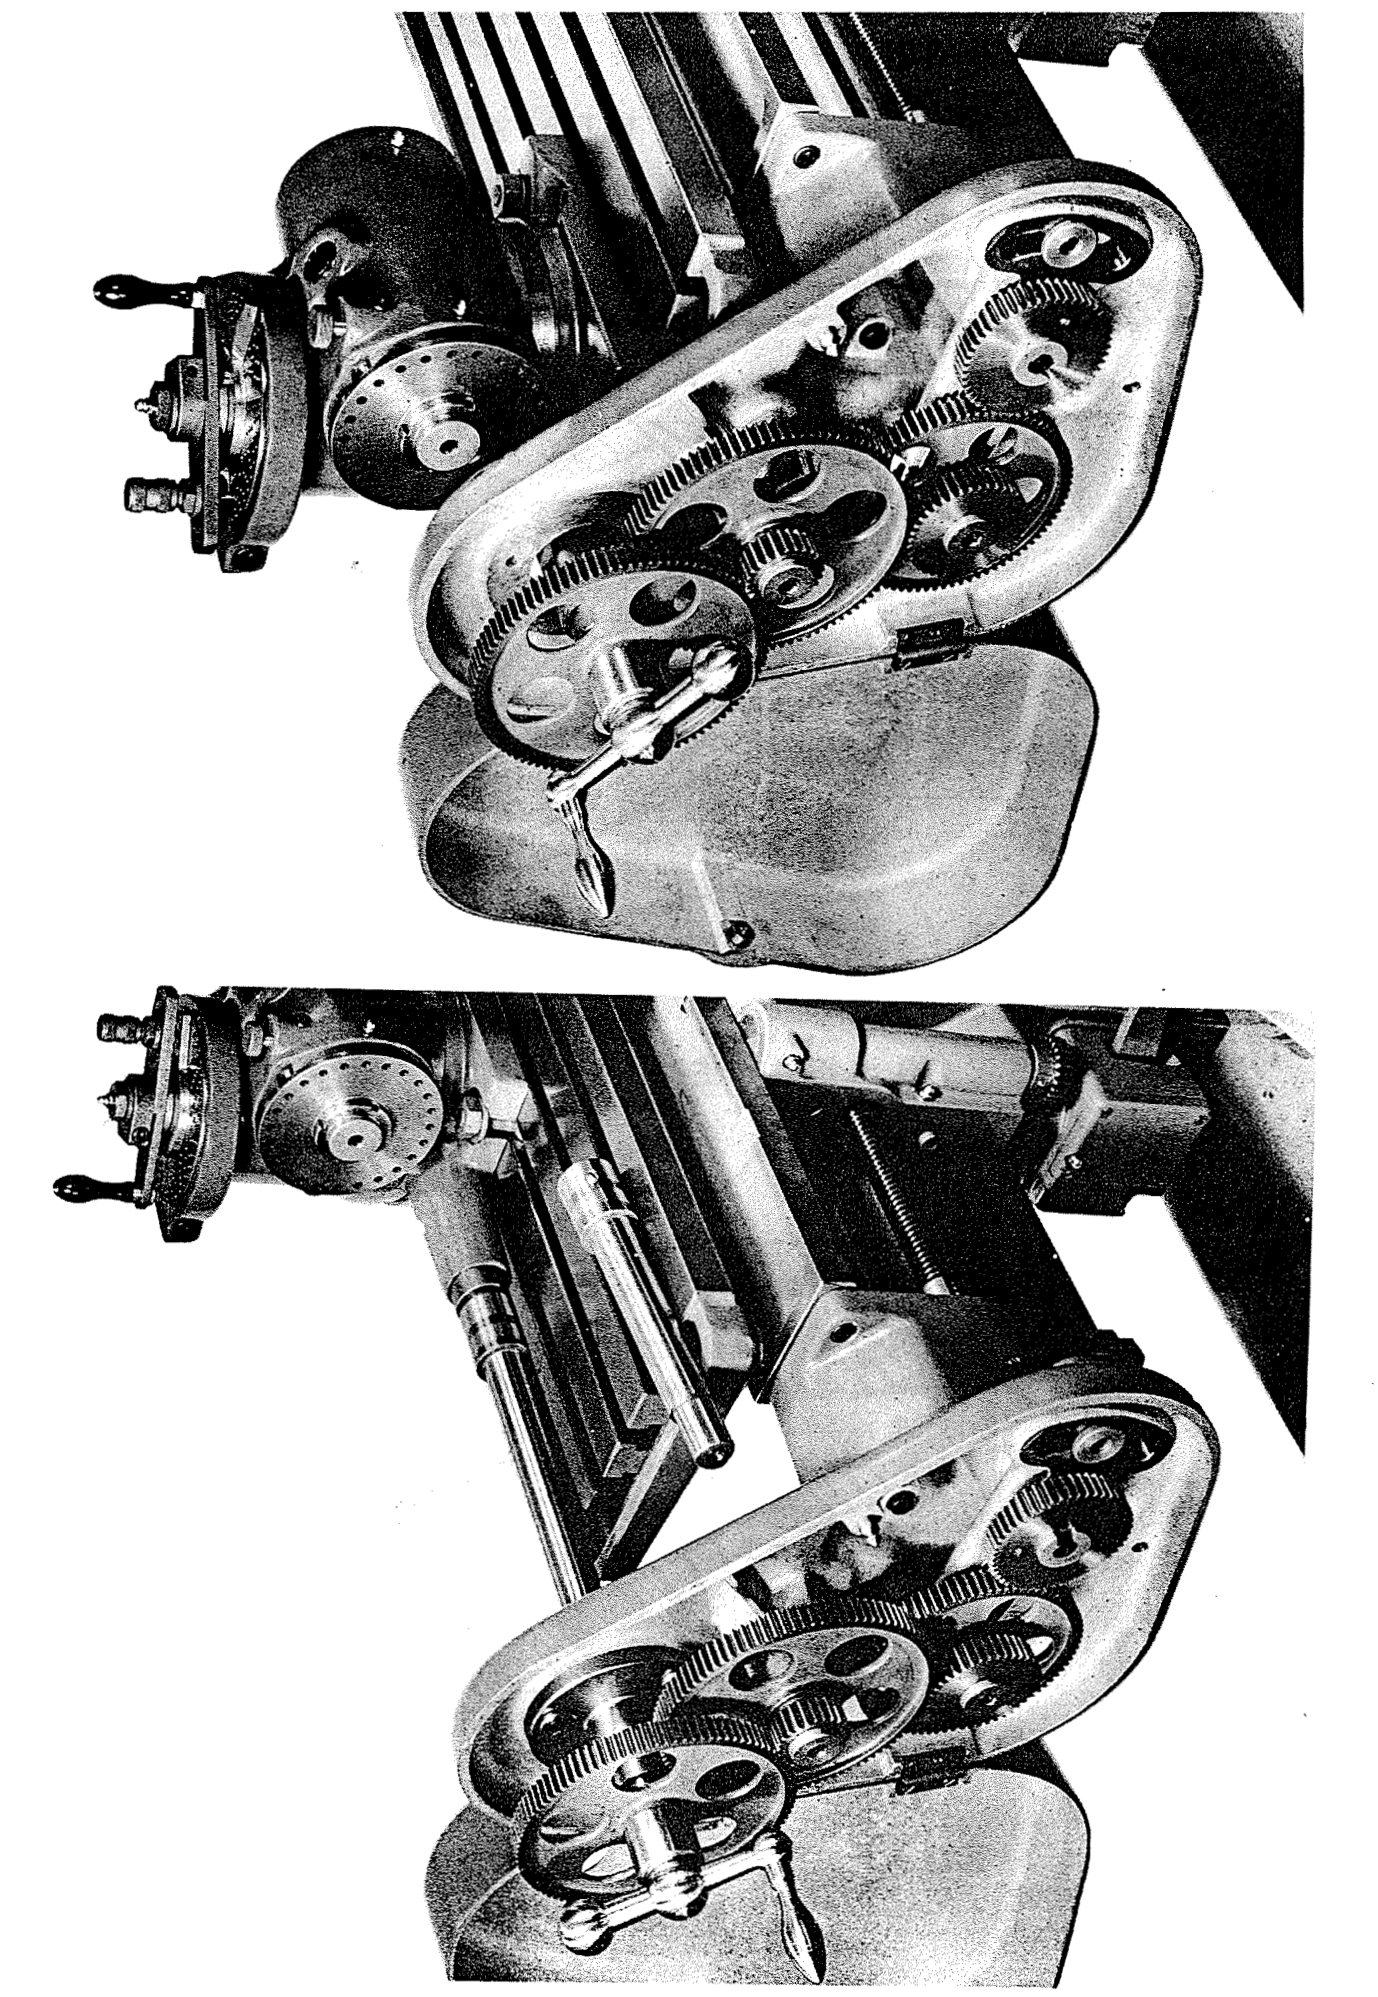
\includegraphics[width=1.0\linewidth]{./images/page_50}
    \caption{Universal Dividing Head Gears}
    \label{fig:universal_dividing_head_gears}
\end{figure}
    \newpage
\begin{figure}[h]
    \centering
    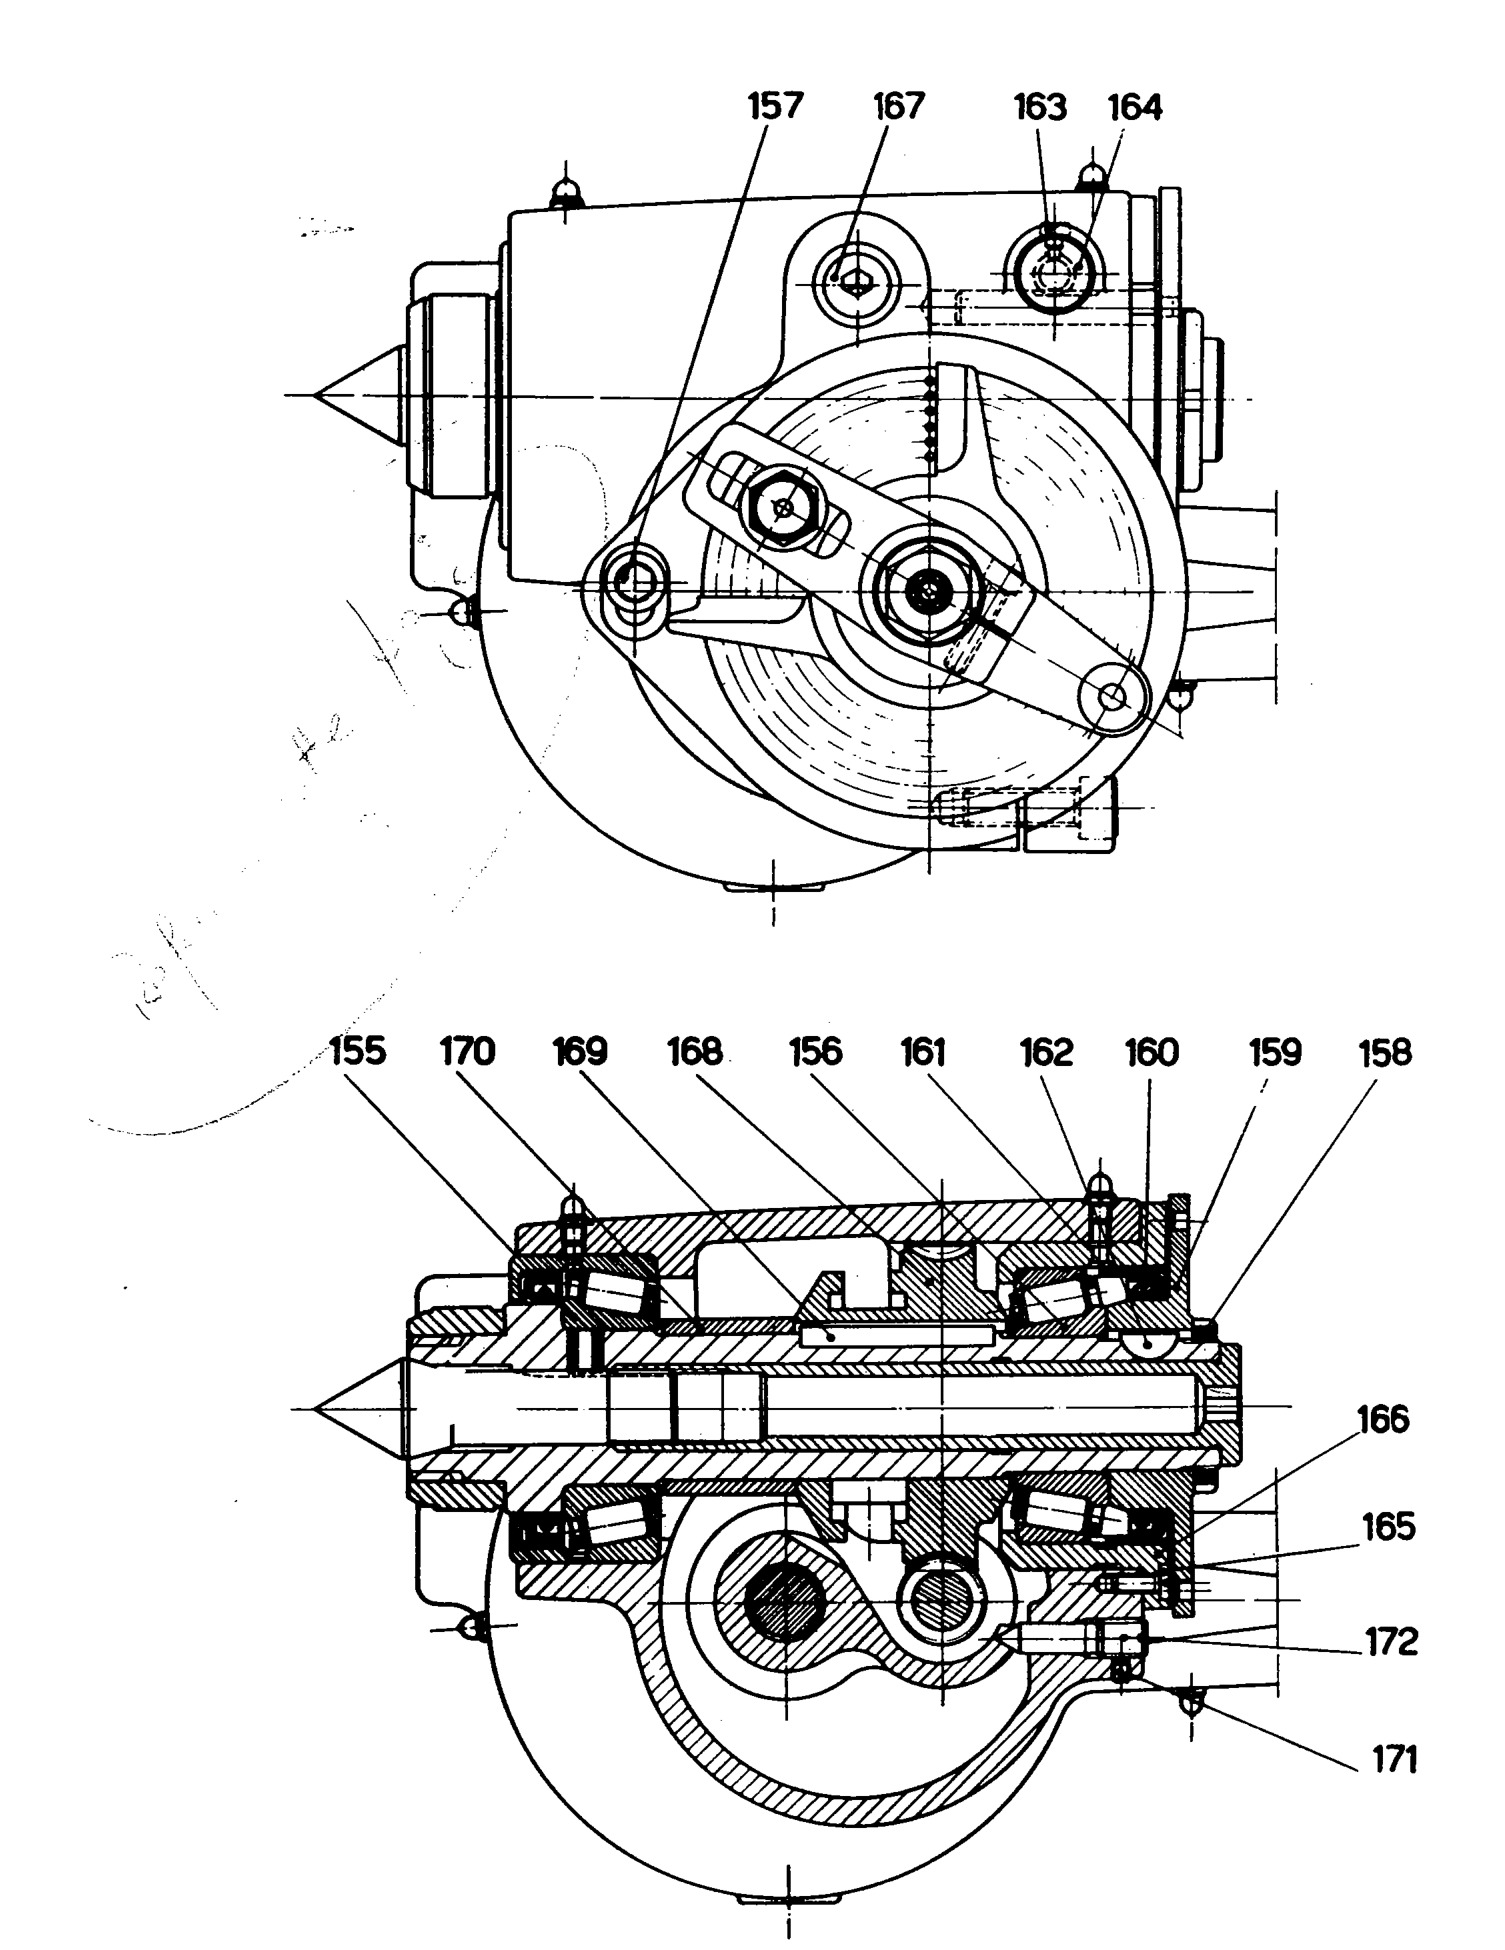
\includegraphics[width=1.0\linewidth]{./images/page_51}
    \caption{Universal Dividing Head}
    \label{fig:universal_dividing_head}
\end{figure}

    \chapter{Kinematic Chain}

% Put the original image on the page
\begin{figure}[h]
    \centering
    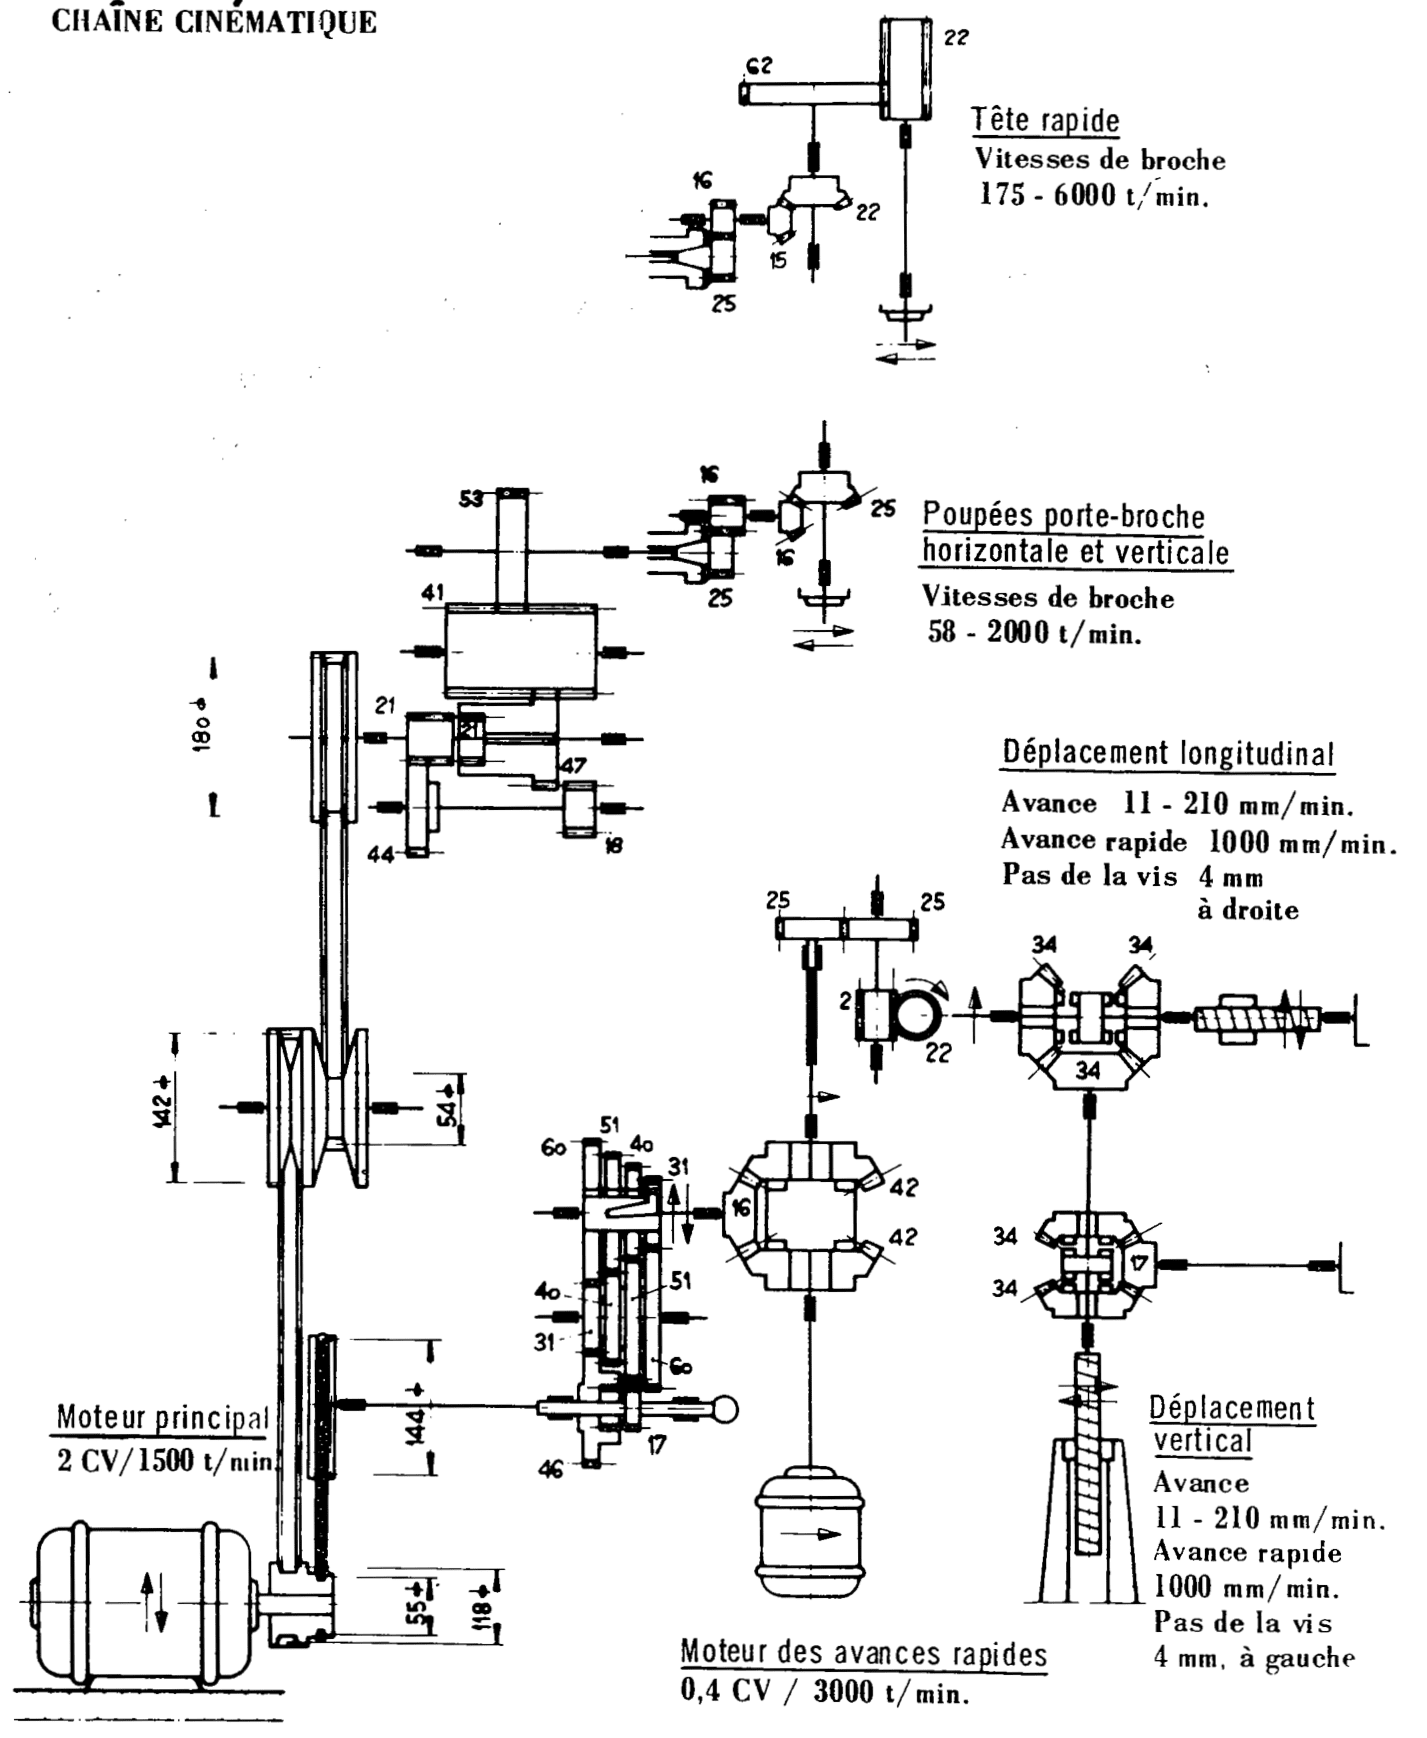
\includegraphics[width=0.95\linewidth]{images/page_56_in_13_36_kinematic_chain}
    \label{fig:kinematic_chain}
\end{figure}

% cover "Chaîne Cinématique with a white box.
\cover{80}{90}{4}{1}

% Default width for label blocks
\newlength{\labelBlockWidth}
\setlength{\labelBlockWidth}{5cm}

% Custom command for label block
\newcommand{\labelBlock}[4][\labelBlockWidth]{%
% Define a label block with white background, bold, and underlined text
    \begin{textblock*}{#1}(#2)
        \colorbox{white}{\parbox{\linewidth}{\uline{#3} \\ \small #4}\vspace{2pt}}
    \end{textblock*}%
}

% Cover "tête rapide" with an English version
\labelBlock{370pt,140pt}{\textbf{High Speed Head}}{Spindle Speeds \\
175 - 6000 r.p.m.}

% cover "Poupées porte-broche horizontale et verticale" with a white box since the new
% text doesn't cover it completely.
\cover{355}{252}{4}{2}
% Cover "Poupées porte-broche horizontale et verticale" with an English version
\labelBlock{355pt,252pt}{\textbf{Horizontal and} \\ \textbf{vertical spindles}}{Spindle Speeds \\
58 - 2000 r.p.m.}

% cover "Déplacement Longitudinal" with a white box since the new
% text doesn't cover it completely.
\cover{370}{330}{4}{2}
% Cover "Déplacement Longitudinal" with an English version
\labelBlock{370pt,335pt}{\textbf{Longitudinal movements}}{Feed: 11 - 210 mm/min \\
Rapid Feed: 1000 mm/min \\
4 mm right-hand thread}

% cover "Déplacement Vertical" with a white box since the new
% text doesn't cover it completely.
\cover{425}{520}{4}{5}

% Cover "Déplacement Vertical" with a white box
\labelBlock[5cm]{425pt,520pt}{\textbf{Vertical movements}}{Feed: 11 - 210 mm/min \\
Rapid Feed: 1000 mm/min \\
4 mm left-hand thread}

% Cover "Moteurs des avances rapides" with an English version
\labelBlock{280pt,600pt}{\textbf{Rapid Feed Motor}}{0.4 HP / 3000 r.p.m.}

% Cover "Moteur Principal" with an English version
\labelBlock[3.3cm]{65pt,535pt}{\textbf{Main Motor}}{2 HP / 1500 r.p.m.}

    \chapter{List of Bearings}
\begin{tabular}{@{}|l|l|l|l|l|l|@{}}
    \toprule
    \textbf{Component}         & \textbf{Count} & \textbf{Type}     & \textbf{Dimensions} & \textbf{Manufacturer} & \textbf{See Page} \\
    \midrule
    \textbf{Frame}             &                &                   &                     &                       &                   \\
    \quad Spindle Gearbox      & 1              & 6307Z             & 35 x 80 x 21        & SKF                   & 2                 \\
    & 1              & 3305              & 25 x 62 x 25.4      & SKF                   & 2                 \\
    & 1              & 30205             & 25 x 52 x 16.5      & SKF                   & 2                 \\
    & 3              & 30206             & 30 x 62 x 17.5      & SKF                   & 2                 \\
    \quad Variable Speed Drive & 1              & 51102             & 15 x 28 x 9         & SKF                   & 3                 \\
    \quad Feed Gearbox         & 2              & 6202              & 15 x 35 x 11        & SKF                   & 12                \\
    & 1              & 6203ZZ            & 17 x 40 x 12        & SKF                   & 12                \\
    & 1              & 6205              & 25 x 52 x 15        & SKF                   & 12                \\
    & 52             & Needle            & 2 x 15,8            & KFA                   & 12                \\
    & 6              & Roller            & 7 x 7               & KFA                   & 12                \\
    \midrule
    Vertical Slide             & 2              & 6002X             & 15 x 32 x 9         & SKF                   & 10                \\
    & 2              & 30203             & 17 x 40 x 13,5      & SKF                   & 8                 \\
    & 1              & 51102             & 15 x 28 x 9         & SKF                   & 10                \\
    & 1              & 51104             & 20 x 35 x 10        & SKF                   & 10                \\
    & 2              & INA-NKIA 5904     & 20 x 37 x 23        & HYDREL                & 10                \\
    \midrule
    Longitudinal Slide         & 2              & 6203Z             & 17 x 40 x 12        & SKF                   & 5                 \\
    & 2              & 30203             & 17 x 40 x 13,5      & SKF                   & 6                 \\
    \midrule
    Horizontal Spindle Head    & 1              & NN 3010 K-Sp      & 50 x 80 x 23        & SKF                   & 13                \\
    & 2              & 100.035 / 100.072 & 35 x 72 x 18,5      & Préc. Indus.          & 13                \\
    & 2              & 51102             & 15 x 28 x 9         & SKF                   & 13                \\
    \midrule
    Vertical Spindle Head      & 1              & Duplex 335 CD EP  & 35 x 80 x 21        & Hoffmann              & 14                \\
    & 1              & 102.035/102.072   & 35 x 72 x 18,5      & Préc. Indus.          & 14                \\
    & 1              & 101.040/101.080   & 40 x 80 x 26        & Préc. Indus.          & 14                \\
    & 1              & INA-NK 20/20      & 20 x 28 x 20        & HYDREL                & 14                \\
    \midrule
    Universal Quick Head       & 2              & 6205              & 25 x 52 x 15        & SKF                   & 15                \\
    & 1              & Duplex 335 CD     & 35 x 80 x 21        & Hoffmann              & 15                \\
    & 2              & 3205-C153         & 25 x 52 x 20,6      & SKF                   & 15                \\
    & 1              & INA-NK 20/20      & 20 x 28 x 20        & HYDREL                & 15                \\
    \midrule
    Mortising Head             & 1              & 6210              & 50 x 90 x 20        & SKF                   & 16                \\
    & 1              & NA 20             & 20 x 42 x 20        & KFA                   & 16                \\
    & 31             & Needle            & 2,5 x 11,8          & KFA                   & 16                \\
    \midrule
    Drilling Device            & 1              & 6204              & 20 x 47 x 14        & SKF                   &                   \\
    \midrule
    Universal Dividing Head    & 1              & 100.035/100.072   & 35 x 72 x 26        & Préc. Indus.          &                   \\
    & 1              & 101.040/101.080   & 40 x 80 x 26        & Préc. Indus.          &                   \\
    \bottomrule
\end{tabular}

    \newgeometry{right=4cm, margin=0cm} % Set top margin to 2cm and all other margins to zero
\begin{landscape}
    \chapter{Lubricating Chart}

    \begin{figure}[ht]
        \centering
        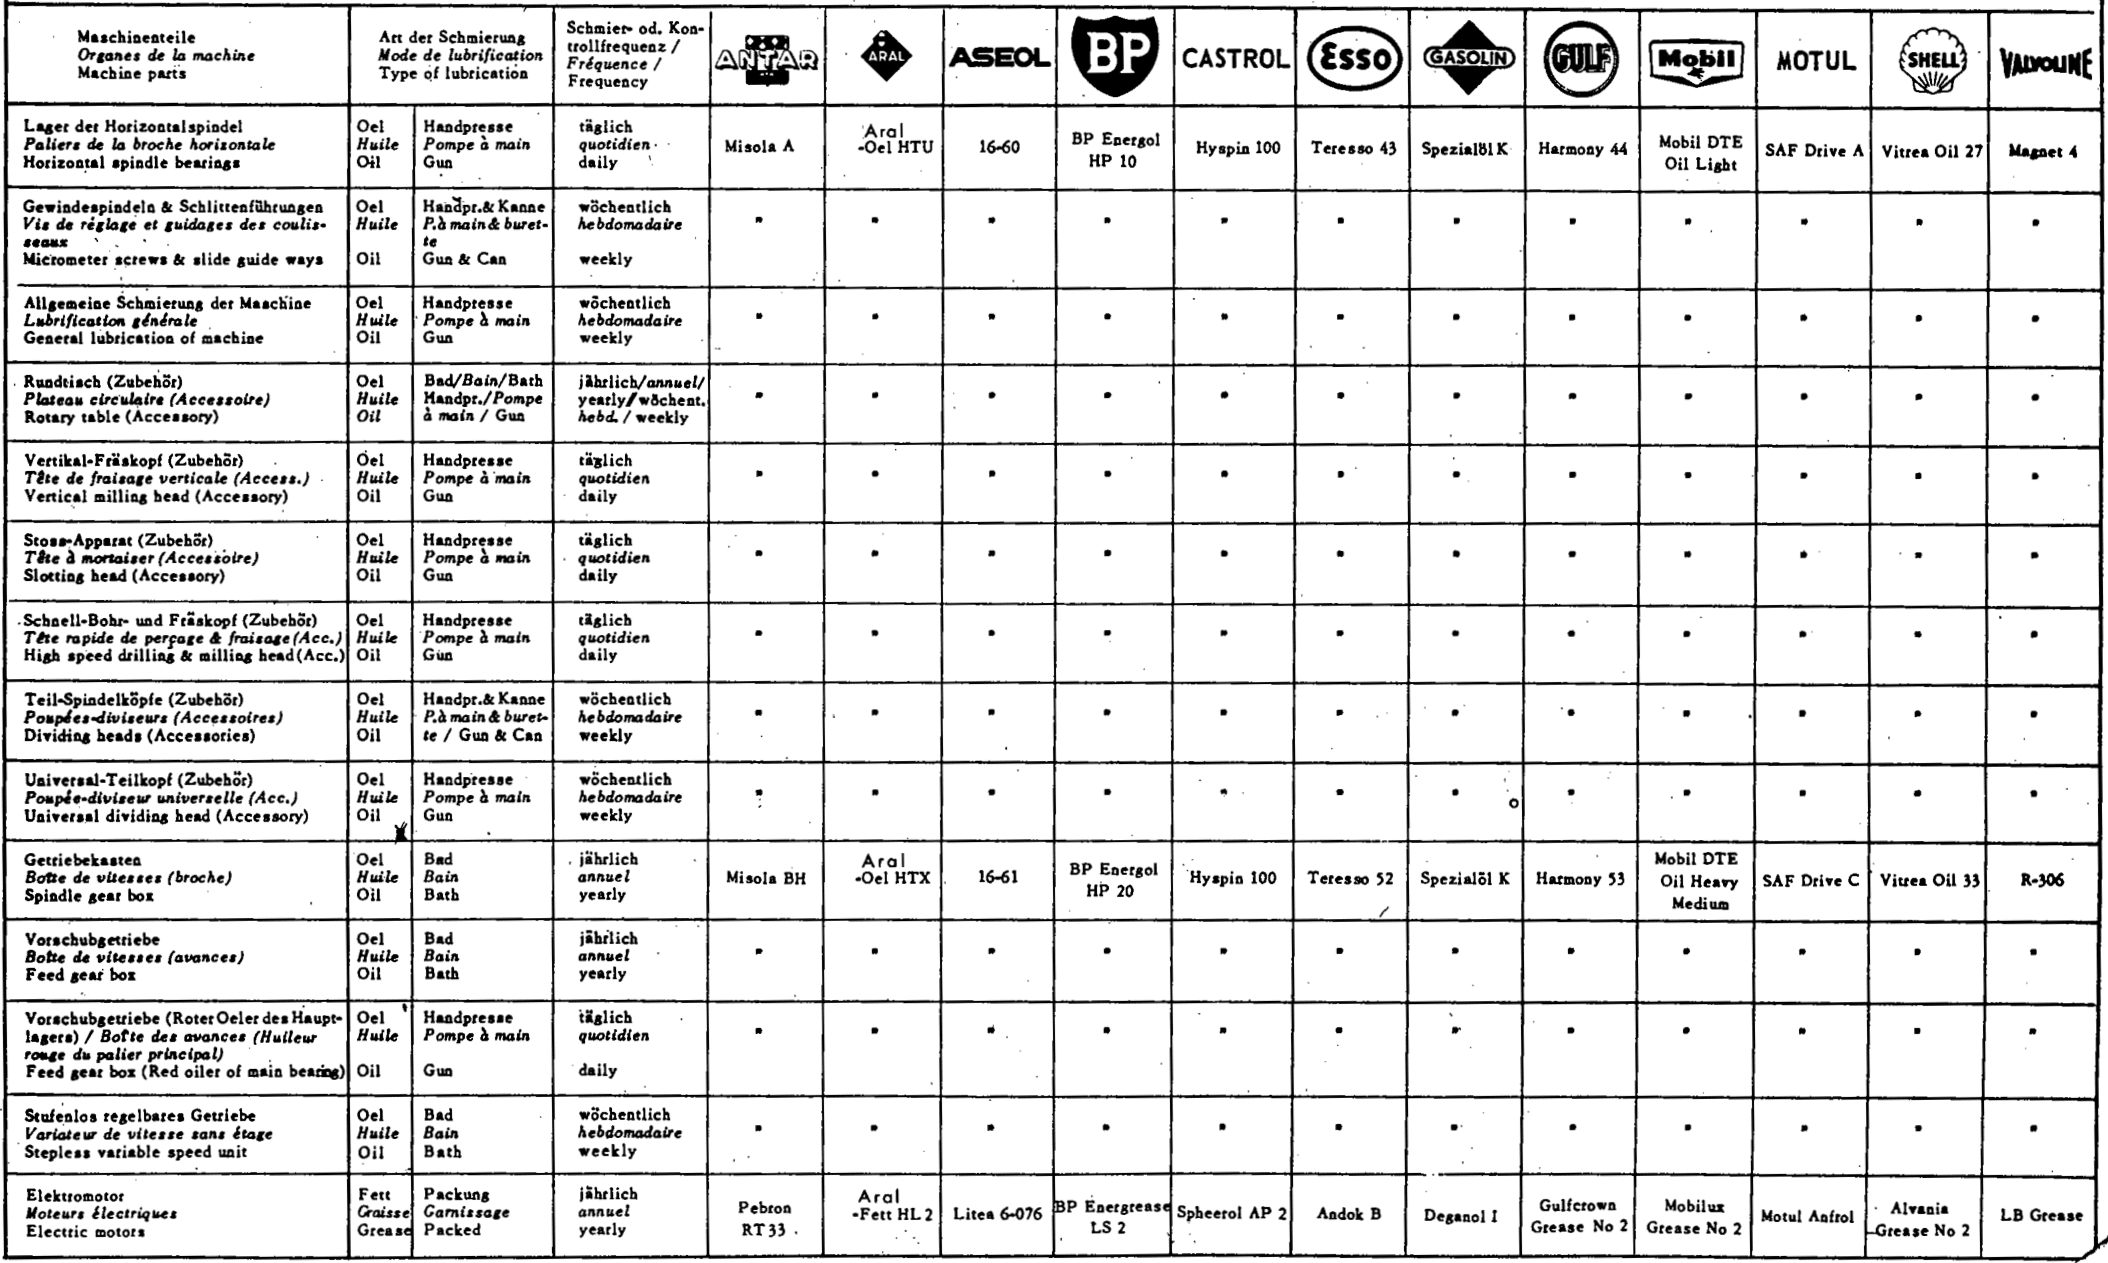
\includegraphics[width=0.9\linewidth]{images/page_58_lubricating_chart}
        \label{fig:lubricating_chart}
    \end{figure}
\end{landscape}
\restoregeometry % Restore normal margins
    \chapter{Lubricating Plan}

\begin{figure}[ht]
    \centering
    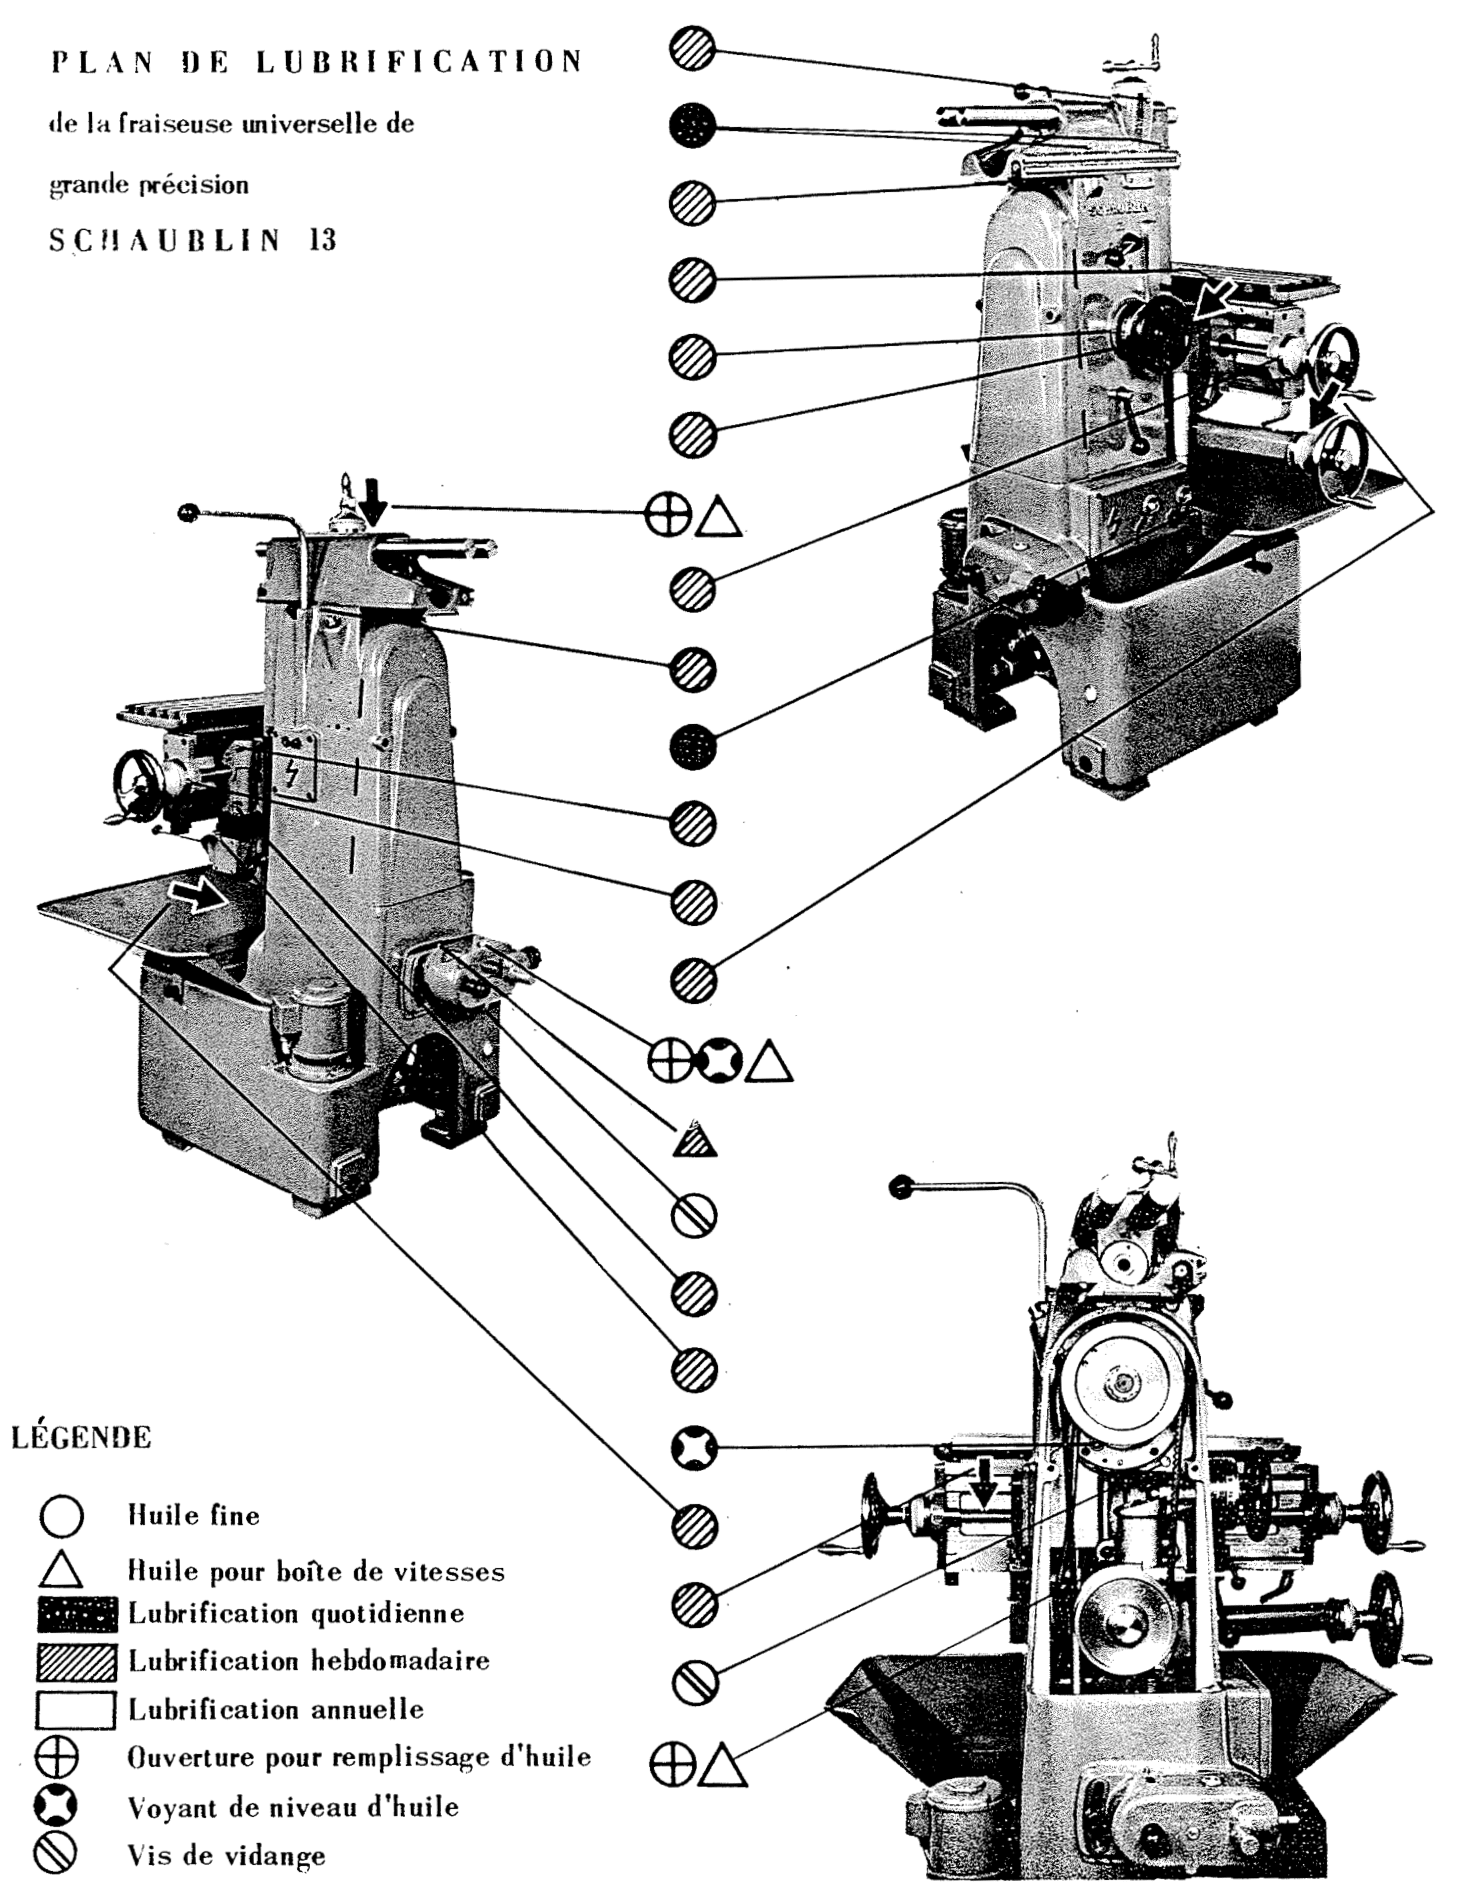
\includegraphics[width=0.9\linewidth]{images/page_59_lubrication_plan}
    \label{fig:lubricating_plan}
\end{figure}

% cover title block with a white box.
\begin{textblock*}{6cm}(100pt, 120pt)
    \colorbox{white}{\textcolor{white}{\rule{6cm}{2cm}}}
\end{textblock*}

% Cover "Légende" with an English version
\begin{textblock*}{3.3cm}(95pt,505pt)
    \colorbox{white}{\parbox{\linewidth}{\uline{\textbf{Legend}}}\vspace{2pt}}
\end{textblock*}

\newcommand{\legendBlock}[2]{%
    \begin{textblock*}{4.5cm}(128pt,#1)
        \colorbox{white}{\parbox{\linewidth}{\small #2}\vspace{2pt}}
    \end{textblock*}%
}

\legendBlock{529pt}{Fine Oil} % Cover "Huile Fine" with an English version
\legendBlock{544pt}{Gearbox Oil} % Cover "Huile pour boîte de vitesses" with an English version
\legendBlock{558pt}{Daily Lubrication} % Cover "Lubrification quotidienne" with an English version
\legendBlock{571pt}{Weekly Lubrication} % Cover "Lubrification hebdomadaire" with an English version
\legendBlock{584pt}{Yearly Lubrication} % Cover "Lubrification annuelle" with an English version
\legendBlock{597pt}{Oil Filling Opening} % Cover "Ouverture pour remplissage d'huile" with an English version
\legendBlock{611pt}{Oil Level Indicator} % Cover "Voyant de niveau de huile" with an English version
\legendBlock{624pt}{Drain Screw} % Cover "Vis de vidange" with an English version

    \chapter{Transmission Components}

\begin{figure}[ht]
    \centering
    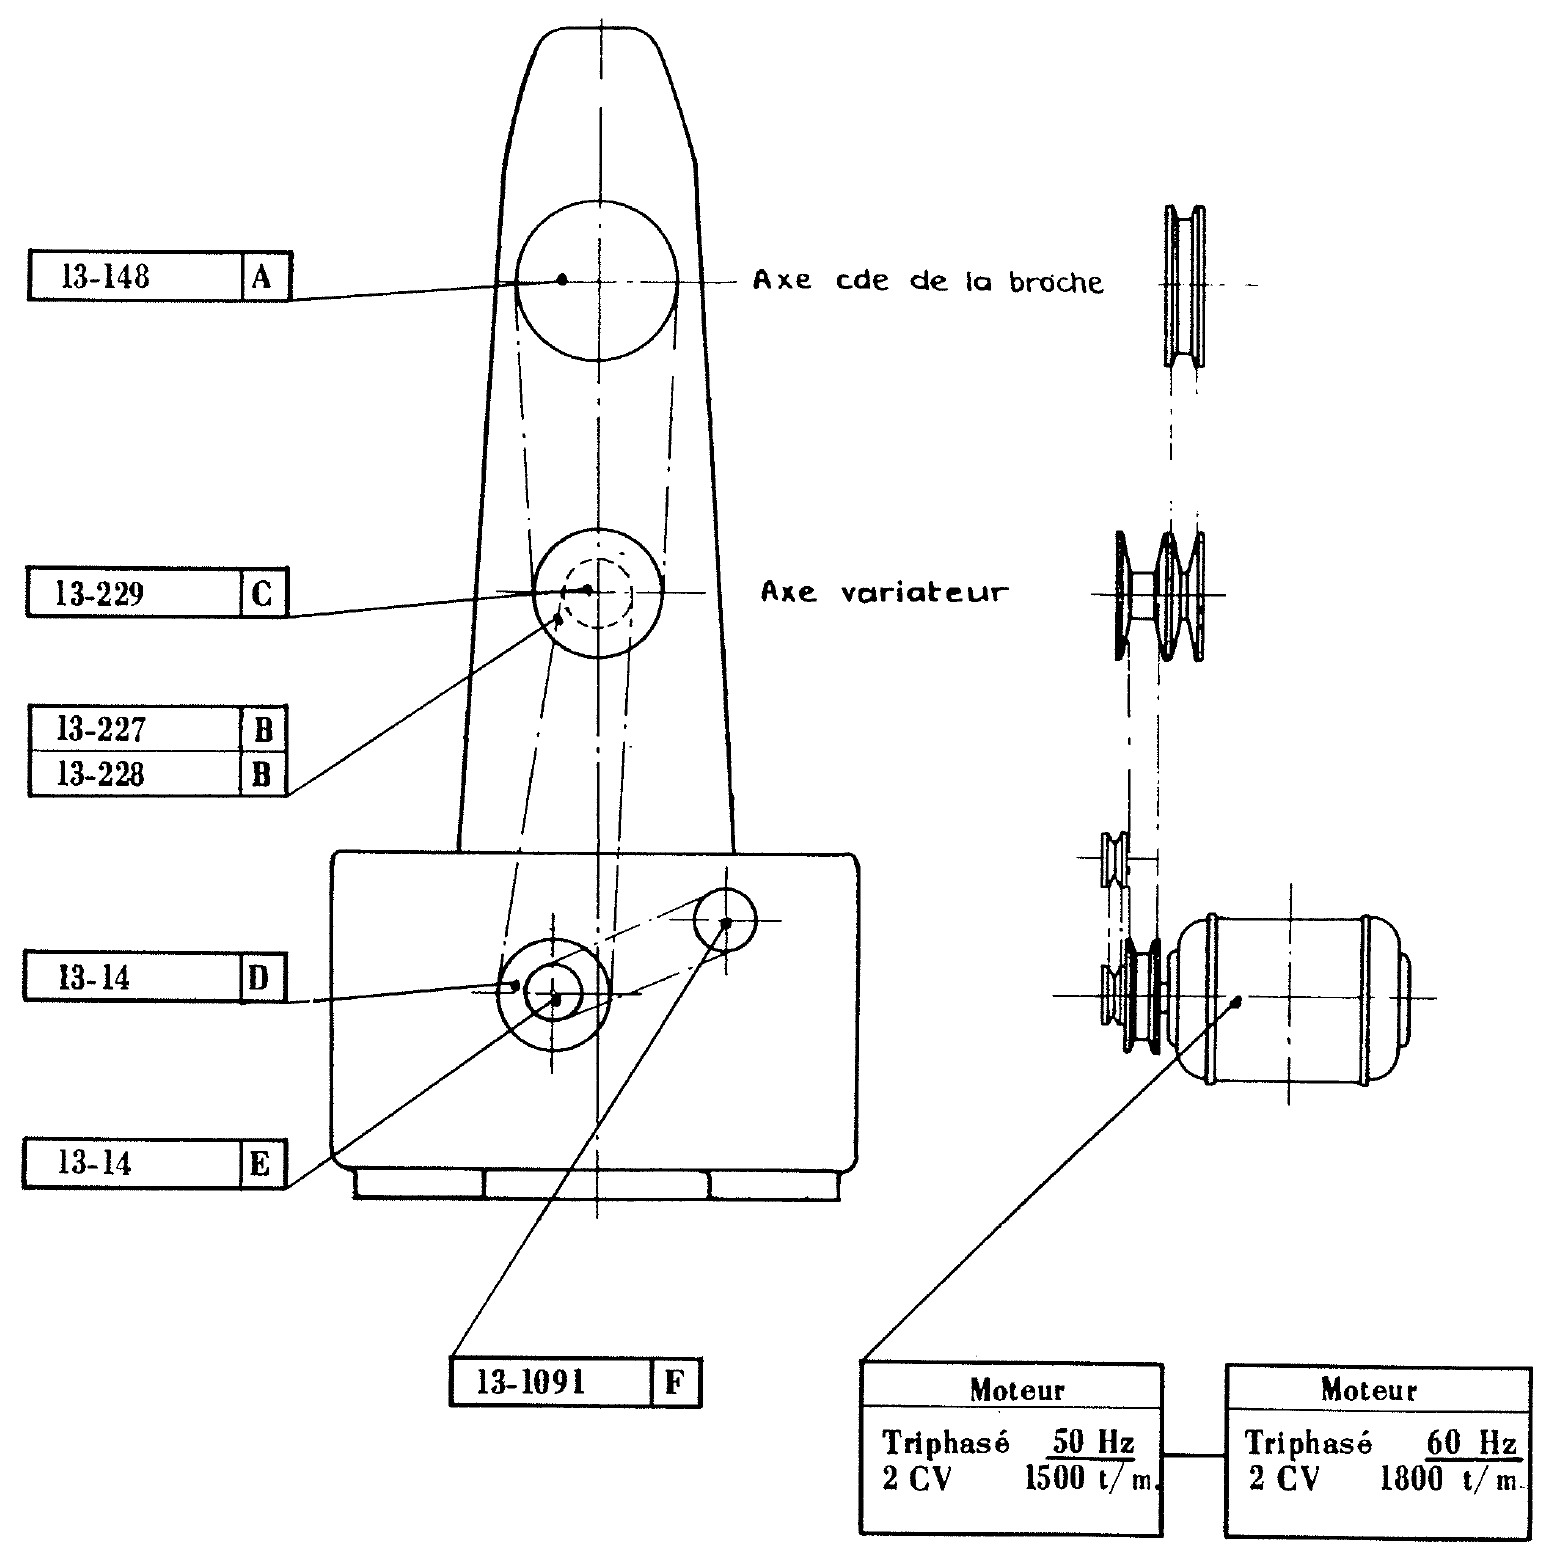
\includegraphics[width=0.9\linewidth]{images/page_60_transmission_components}
    \label{fig:transmission_components}
\end{figure}


\cover{290}{180}{3.1}{.5}

\begin{textblock*}{2cm}(310pt,180pt)
    \colorbox{white}{\parbox{\linewidth}{\small Spindle Axis}\vspace{2pt}}
\end{textblock*}%


\cover{290}{250}{3.1}{.5}

\begin{textblock*}{2.5cm}(300pt,260pt)
    \colorbox{white}{\parbox{\linewidth}{\small Variator Axis}\vspace{2pt}}
\end{textblock*}%

\newcommand{\transmission}[4][.5]{%
    \def\coverXPosition{\numexpr #2 - 3\relax}
    \def\coverYPosition{\numexpr #3 - 4\relax}
    \cover {\coverXPosition}{\coverYPosition}{2.5}{#1}

    {\small
        \begin{textblock*}{4cm}(#2pt,#3pt) % width and position (x, y)
            \begin{tabular}{|p{1.5cm}|c|}
                \hline
                #4
                \hline
            \end{tabular}
        \end{textblock*}
    }%
}

\newcommand{\motor}[3]{%
    \def\coverXPosition{\numexpr #1 - 3\relax}
    \def\coverYPosition{\numexpr #2 - 4\relax}
    \cover {\coverXPosition}{\coverYPosition}{3.2}{2}

    {\small
        \begin{textblock*}{4cm}(#1pt,#2pt) % width and position (x, y)
            \begin{tabular}{|l|}
                \hline
                #3
                \hline
            \end{tabular}
        \end{textblock*}
    }%
}

\transmission{98}{178}{13-148 & A \\}
\transmission{98}{261}{13-229 & C \\}
\transmission[1]{98}{295}{13-227 & B \\ \hline 13-228 & B \\}
\transmission{98}{362}{13-14 & D \\}
\transmission{98}{410}{13-14 & E \\}
\transmission{210}{470}{13-1091 & F \\}

\motor{305}{470}{Motor \\ \hline Three-phase 50Hz \\ 2HP 1500 r.p.m. \\}
\motor{410}{470}{Motor \\ \hline Three-phase 60Hz \\ 2HP 1800 r.p.m. \\}

{\small
    \begin{tabular}{|c|c|c|c|c|c|c|c|c|c|c|}
        \hline
        \multicolumn{6}{|c|}{\diameter Pulleys (mm)} & \multicolumn{5}{|c|}{Belts (mm or inch)} \\
        \hline
        A   & B      & C      & D   & E  & F   & Connection & Inner length & Profile       & Manufacturer & Identification   \\
        \hline
        181 & 146-54 & 146-54 & 119 & 51 & 140 & A/B        & 47 1/2"      & 1 x 11/32"    & Dayton       & S2268            \\
        &        &        &     &    &     & C/D        & 47 1/2"      & 30\textdegree & Dayton       & S2268            \\
        &        &        &     &    &     & E/F        & 725          & 10/6          & Pallas       & N\textdegree  6172 \\
        \hline
    \end{tabular}
}
    \chapter*{NOTE on the Maintenance of Coolant Pumps}

The coolant pump should be thoroughly cleaned for single-shift operation at least 2 times a year and for multi-shift operation at least 3 times a year.
For this purpose, it must be completely disassembled. All parts should be carefully cleaned in petroleum or benzine.
Tanks, pipes, grids, and filters should also be cleaned thoroughly.

Neglecting maintenance leads to rapid wear of the pump, especially when using so-called "soluble" oil emulsions.

The pump gland packings should be adjusted correctly or replaced if necessary.
For work without coolant fluid, the pump should be taken out of service.
Running the pump without liquid quickly causes serious defects.
If, even after observing the rules above, the pump continues to cause problems, it should be attributed to:

\begin{enumerate}
    \item The lubricant, especially the emulsion, is not changed frequently enough.
    Due to decomposition, the fatty part of the emulsion, together with chips (especially light metal chips) and other impurities,
    forms a sticky mass that clogs grids, filters, pipes, and fittings.
    \item The tanks are not thoroughly cleaned when changing the coolant fluid, so the new mixture becomes unusable immediately.
    \item Often, due to forgetfulness or negligence, the pump is not stopped, even when there is no suction of liquid.
    Due to its silent operation, it runs during breaks and often 24 hours a day.
\end{enumerate}

\textbf{The electric pump is an important and necessary accessory for all machine tools.}

It is used to bring the coolant fluid to the point where chip removal occurs to remove the heat generated,
lubricate, protect the machined surface from rust and corrosion, and also evacuate the chips during machining.

This process increases both cutting efficiency and tool life.
On the actual work, a good supply of coolant fluid influences precision and finishing quality.

    \chapter{Installation, Commissioning, and Maintenance Instructions for Alternating Current Motors}

\begin{figure}[ht]
    \centering
    
\includegraphics[width=0.1\linewidth]{images/page_62_manufacturer_logo}
    \label{fig:alternating_motor_manufacturer_logo}
\end{figure}

{\small

\section*{1. Installation}

The installation of motors depends on the conditions in which they are intended to operate.
Normal-type, \textbf{protected, ventilated} motors should only be installed in dry and non-dusty areas.
\textbf{Special insulation motors} should be used in areas where water condensation, dust, or aggressive gases may occur.
For operations where our standard motors are not suitable, we have developed special types (motors with a protective cap against water droplets,
    enclosed motors with or without fresh air intake, etc.).

During installation, consideration should be given to the accessibility of parts that may require periodic inspection,
    such as bearings, brushes, terminal plate, short-circuit device, etc.

It is advisable to mount the motor on a concrete base, directly or on slides.
The rotor axis, especially for motors with plain bearings and lubrication by rings, \textbf{must be perfectly horizontal and parallel to the shaft it is intended to drive.}

If the motor is mounted on slides, it is better to first screw them onto the motor, then place the assembly on the base,
    place shims under the slides, and finally seal them.
When the installation is complete, tighten the motor fixing screws to the slides or base, taking care not to twist the motor frame.

In the case of \textbf{belt drive}, the center of the motor pulley and the driven pulley must be perfectly in the same plane.
The belt should not be too tight, otherwise, the bearings would be subject to excessive pressure and could \textbf{overheat}.

\textbf{Ball bearing motors} can be mounted against a wall or ceiling, even in a vertical or inclined position if necessary,
    provided that, apart from the weight of the pulley or coupling, the motor shaft is not subject to any other axial force.

In such cases, the bearing flanges of \textbf{ring-lubricated motors} must be turned 90° or 180° so that the oil filling opening is always at the top.

The motor shaft ends are machined according to the \textbf{VSM tolerance system} (Swiss Society of Machine Builders),
    \textbf{light pressed fit k5}, and equipped with a keyway with a key according to VSM standards.
The parts to be mounted on the shaft ends must have a normal H6 bore.
This adjustment has been adopted because the forcing resulting from a tight fit easily causes excessive axial loads on the bearings.
The faces of the shaft ends are drilled with a threaded hole (see figures 3 and 4) to allow the axial fixing
of transmission components such as pulleys, gears, couplings, etc., with a washer and screw.

The installation of pulleys, gears, couplings, etc., on the shaft ends is done using a screw inserted into the threaded
hole and an appropriate device. When pulleys, etc., are not supplied by us, care should be taken to ensure that they are carefully balanced.

\section*{2. Connection}

Before connecting the motor, check if the voltage indicated on the nameplate matches the network voltage.
Connect the motor according to the instructions on the diagram supplied with the motor or attached inside the terminal cover.
Grounding is done by the yellow screw.

    \begin{wrapfigure}{R}{0.35\textwidth}
        \centering
        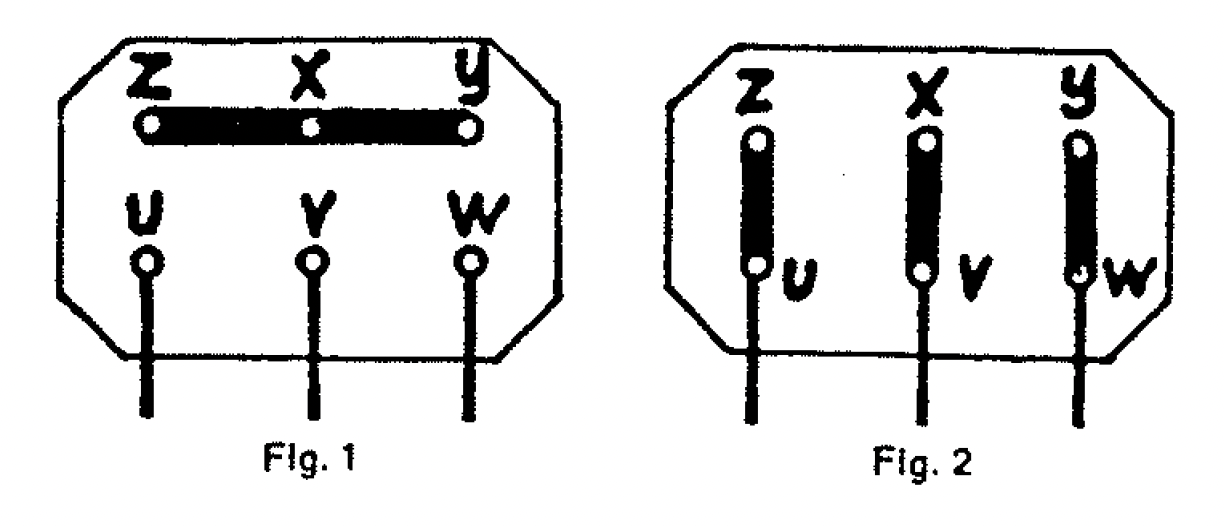
\includegraphics[width=0.33\textwidth]{images/page_62_alternating_motor_connections}
        \label{fig:alternating_motor_connections}
    \end{wrapfigure}

    The motor stator typically has a terminal plate with 6 terminals to which the phase arrivals and departures are connected.
    If it is a three-phase motor designed for two voltages E and E V3,
    connections should be made as indicated in Figure 1 for the higher voltage (star connection) and,
    for the lower voltage (delta connection), according to Figure 2.

\section*{3. Rotation Direction}

To reverse the rotation direction, simply swap two of the current leads at the stator terminals;
for three-phase motors: two current leads, for biphasic motors with compound voltage: the two outer conductors,
    for biphasic motors with non-compound voltage and single-phase motors: two current leads from the same phase.
    If the motor is equipped with a double-width pulley for driving a fixed pulley and idle pulley, the belt must be on the idle pulley at startup.
The belt should be brought onto the fixed pulley only when the motor has reached its full speed.
Unless the motor has a third bearing (external), the belt must always rotate on the bearing flange side.
If the motor stops for any reason, it must be immediately switched off to prevent damage.
Maximum temperatures: bearings, about 50\textdegree C; windings and iron, 80\textdegree C above ambient temperature (max. 40\textdegree C).

\section*{4. Maintenance}

All our \textbf{ball bearing motors} are supplied with enough grease to last approximately 6 to 12 months under normal operating conditions.
A good ball bearing grease should be used, which will be pumped into the bearings using Stauffer or Técalémit "S" grease fittings (figure 3).


    \begin{wrapfigure}{L}{0.35\textwidth}
        \centering
        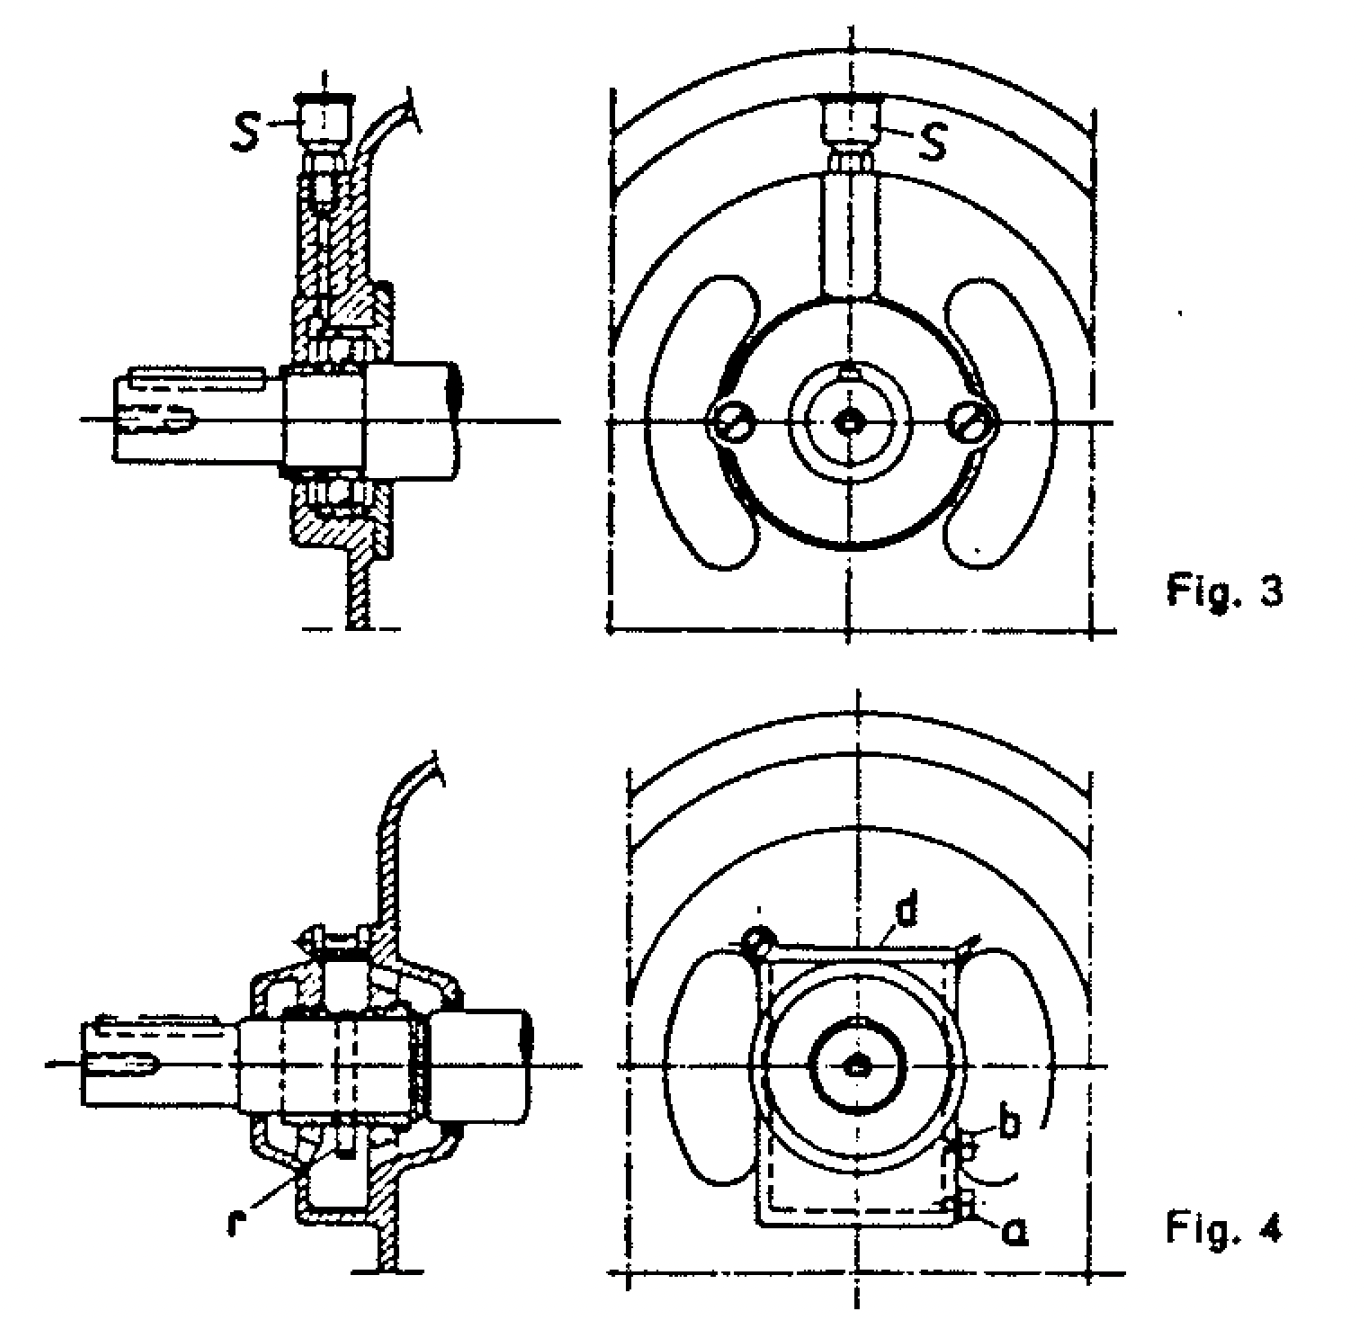
\includegraphics[width=0.33\textwidth]{images/page_62_maintenance}
        \label{fig:alternating_motor_maintenance}
    \end{wrapfigure}

    \textbf{Bearing ring motors} are shipped without oil.
    Before commissioning, it is recommended to clean the oil chambers with gasoline and, when dry, fill them with resin- and acid-free machine oil.
This initial oil charge will be renewed about 1 month later and then again 2 to 4 months later.
Afterward, the oil should be changed every 6 months. To do this, drain the oil by removing screw "a" (Figure 4) and clean the oil chamber with gasoline. Then, replace screw "a," loosen screw "b," and pour in new oil until it overflows through overflow "b." Replace screw "b" and close the bearing cover.

It is absolutely essential that the oil feed ring "r" comes with the shaft and transports oil. Periodically check its condition and purity.

For \textbf{motors with ring-induced}, occasionally check if the rings are still smooth and free of carbon dust. Spark production can result from ovalization of the rings, burns, improper brush support, insufficient brush pressure, brushes or support rods having play, or vibrations due to improper motor installation.

If the rings are only slightly ovalized, burned, or dirty, simply sand them with emery or glass paper using a wooden piece that matches the curvature of the rings. If the rings are considerably damaged, it will be necessary to grind and then polish them on a lathe. Never apply paraffin, grease, etc., to the rings.

If the brushes do not press with their entire surface on the rings, they should be sanded by placing a piece of emery cloth on the rings and moving it back and forth under the brushes until the contact surface of each brush perfectly matches that of the ring.

Carefully remove carbon and metal particles, dust, etc., and wipe the rings with a dry cloth. Repeat the same process when installing new brushes. Since bronze brushes are relatively hard, it is preferable to give them a curvature corresponding to that of the rings using a half-round file, and then finish this work with emery cloth. Slightly chamfer the edges of the brushes to avoid spark production at these points.

The wear of brushes and rings in \textbf{fixed-brush} motors is naturally higher than in motors with \textbf{ring short-circuiting and brush lifting devices}. Always keep the short-circuiting contacts of the rings and the rotor starter clean and lightly grease them with Vaseline. Remove any fusion beads that may occur using a file and emery paper.

\section*{5. Spare Parts}

When ordering spare parts such as bearings, plain bearings, brush holders, brushes, etc., it is essential to specify the manufacturing number and type of the motor found on the nameplate. In case of doubt (especially for older motors), send a model of the desired part to the factory.

Replacement brushes must absolutely be of the same brand as those delivered with the motor. When ordering brushes, also specify their brand and dimensions (for example, SR 81, 16 x 32 mm). In case of disputes, it is better to send a few used brushes to our factory, as their appearance often helps identify the cause of the disputes.

}
    \chapter{Service Instructions for Alternating Current Motors with Short-Circuit Rotor}

\begin{figure}[ht]
    \centering
    
\includegraphics[width=0.1\linewidth]{images/page_63_manufacturer_logo}
    \label{fig:schindler_manufacturer_logo}
\end{figure}

\begin{center}
    \textbf{\small SCHINDLER \& CIE. S.A. EBIKON-LUCERNE, SWITZERLAND}
\end{center}


\section*{1. Installation}

The motor will be placed as much as possible in a place free of dust and humidity;
it should be fixed, plumb, on a metal or concrete base (or wood for small motors).

The motor and device housings must be grounded.

The motor connection will be made according to the connection diagram attached to each machine.
The motor must be protected according to the intensity indicated on the plate and according to the starting conditions.

For installations with a double-width pulley, make sure that, during loaded operation, the belt is on the motor side.

As a transmission element, glued, leather, or balata belts will be used. The use of staples should be avoided.
Axial shocks of the rotor are an indication of a deformed belt. To prevent bearing heating, the belt should not be too tight.
If the pulley needs to be replaced or if a second pulley is key-seated on the other end of the shaft,
make sure that these pulleys are well balanced.
Dismounting or keying of the pulleys must be done carefully to avoid damaging the bearings.

\section*{2. Commissioning}

Before commissioning, the sleeve bearings must be carefully cleaned with petroleum.
The latter will be introduced through the bearing cover and will flow out through the drain hole whose cap will have been unscrewed.
This operation will be repeated until the petroleum flows clear through the drain hole.

    After being cleaned, the bearings will be filled with high-quality mineral oil, free of acid and not too fluid.
Before filling, close the drain hole and unscrew the overflow plug located on the side of the bearing.
Pour the oil into the bearings until it overflows from the overflow, which will then be closed with its plug.
The overflow level should not be exceeded, as excess oil may flow into the motor, or the lubricating rings will remain stationary.
Ensure that the rings rotate and stir the oil.

Ball or roller bearings are filled with grease in our factories and delivered ready for operation.
No lubrication device is provided, as it could be a risk of contamination, with new grease being introduced
into the bearing without flushing out the old, contaminated grease.
Additionally, it is impossible to verify if the grease enters the motor, which could have its disadvantages.

The rubbing surfaces of the devices must be carefully cleaned.
Check if the connections are made exactly according to the diagram.
The stator has a 6-terminal plate to which the inputs and outputs of each phase will be connected.

If a three-phase motor is designed for 2 different voltages \(E\) and \(\sqrt{3}E\), the connections will be made:
In star, according to Figure 1, for the higher voltage indicated on the plate, and in a triangle, according to Figure 2,
for the lower voltage.

\begin{figure}[ht]
    \centering
    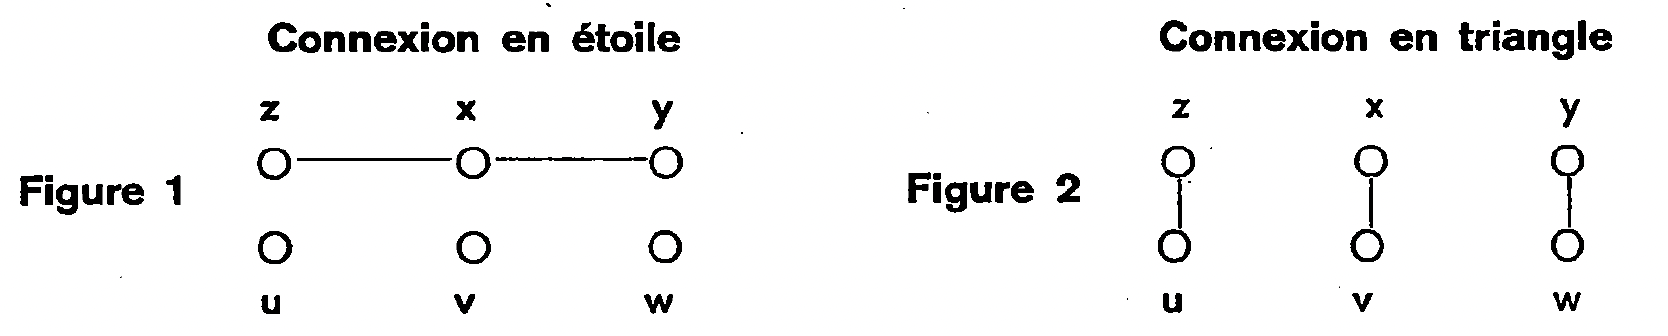
\includegraphics[width=1\linewidth]{images/page_64_motor_connections}
    \label{fig:schindler_motor_connections}
\end{figure}

To reverse the direction of rotation, it is sufficient to interchange two of the current supply wires at the terminal plate:

\begin{itemize}
    \item For three-phase motors: any two supply wires
    \item For two-phase motors with compound voltage: the two outer conductors
    \item For two-phase motors with non-compound voltage and single-phase motors: any two supply wires of the same phase
\end{itemize}

If the motor stops, it must be immediately disconnected. The maximum temperature should not exceed \(35^\circ C\) above
the ambient temperature. Refer to the diagram for details.

If the motor with a double-width pulley is intended for transmission with fixed and loose pulleys,
the belt must be on the loose pulley at startup and move to the fixed pulley only when the motor reaches its speed.

\section*{3. Maintenance}

The motor must be cleaned 1 or 2 times a year when it is out of operation, using a bellows or compressed air,
and then wiped with a cloth soaked in benzene. It is essential to avoid the penetration of oil or impurities into the winding.
Do not damage the insulation, and check if all terminals and nuts are securely tightened.

The sleeve bearings must be filled with oil as consumption occurs, and every 5 to 6 months, the oil must be renewed.
To prevent dust or dirt from falling into the bearings, wipe the covers before opening them. If necessary,
the bearings should be cleaned with petroleum.

Ball bearings consume very little grease, and one filling is expected to last for about 10,000 hours of operation.
After this period, but at least every 3 years, perform a new filling as follows:


    \section*{4. Maintenance}

After removing the outer cover of the bearing and loosening the screws fixing the bearing flanges to the frame,
the flanges can be moved, leaving the bearings easily accessible and fixed on the shaft.
Remove the old grease from the covers and shields by washing them with petroleum.
Then, fill the covers and bearings about three-quarters full with new grease and reassemble everything,
putting each piece back in its original position before disassembly.
It is essential to avoid the introduction of water or dust into the bearings; the seals should be in good condition,
and the screws tightened. Only use high-quality grease, free of acid, retaining its lubricating qualities at high temperatures
as well as in cold conditions.
The replacement of pads or ball bearings is determined by the air gap (clearance between the stator and rotor),
which should not be less than 0.1-0.2 mm. This gap can be checked using a gauge that we can provide upon request.

All parts are manufactured according to gauges and are, therefore, interchangeable.
In case of ordering any spare parts, it is sufficient to indicate the manufacturing number marked on the motor plate.

\section*{4. Faults and Their Causes}

\subsection*{1. Bearing Overheating}
\begin{itemize}
    \item Defective assembly when the motor is directly coupled with a machine, and the two shaft ends are not aligned.
    \item Insufficient cleaning of bearings before commissioning.
    \item Grease rings not rotating; the oil is too thick or excessive in the bearings.
    \item Poor-quality, impure, or insufficient oil.
    \item Too much or too little grease or poor-quality grease in the bearings.
    \item Belt too tight, or in the case of a double-width pulley, the belt under load is too far from the bearing.
\end{itemize}

\subsection*{2. Oil Losses at the Bearings}
\begin{itemize}
    \item Excessive oil in the bearings.
    \item Oil channels are obstructed.
    \item The drain screw is not sufficiently tightened.
\end{itemize}

\subsection*{3. Abnormal Motor Noise}
\begin{itemize}
    \item Cut in a pipeline (defective fuse, poor contact, or lack of contact at the switch, disconnected connections on the terminal board).
    \item Short circuit between windings.
    \item Bearings misaligned due to wear.
\end{itemize}

\subsection*{4. Excessive Motor Heating}
\begin{itemize}
    \item Due to overload (excessive current).
    \item Insufficient motor cooling (surrounded by a partition).
    \item Voltage too high.
    \item Ventilation channels clogged.
    \item Short circuit in windings.
\end{itemize}

\subsection*{5. Motor Stops}
\begin{itemize}
    \item Due to overload.
    \item Too low voltage.
    \item Interruption in a pipeline (defective fuse, poor or no contact at the switch).
    \item Seizure of plain bearings or defective bearings.
\end{itemize}

\subsection*{6. Abnormal Number of Revolutions}
\begin{itemize}
    \item Due to overload.
    \item Interruption in a phase.
    \item Frequency deviations.
\end{itemize}

\begin{flushright}
    Fabrique d'Ascenseurs et de Moteurs Electriques\\
    \textbf{SCHINDLER \& CIE. S.A. EBIKON-LUCERNE}\\
    Phone (041) 6 21 21\\
    Phone (041) 6 31 31
\end{flushright}

    \chapter{Schaublin 13 Milling Machine Drawings}

This attachment comprises a comprehensive collection of drawings meticulously sourced from the original French version of the Schaublin 13 milling machine manual. These drawings, provided by Schaublin, offer an in-depth insight into the intricacies of the machine, serving as a valuable resource for users seeking detailed visual references. Each drawing has been faithfully reproduced to maintain the integrity of the original technical documentation.

\textbf{Key Points:}
\begin{enumerate}
    \item \textbf{Comprehensive Set:} The attachment includes a thorough compilation of drawings encompassing all aspects of the Schaublin 13 milling machine.

    \item \textbf{Original Source:} Drawings are sourced directly from the authentic French version of the Schaublin manual, ensuring accuracy and reliability.
\end{enumerate}

Feel free to utilize this attachment to enhance your understanding of the Schaublin 13 milling machine, utilizing the wealth of technical information provided in the original documentation.

\newpage


\section{Longitudinal lead screw}

\begin{figure}[ht]
    \centering
    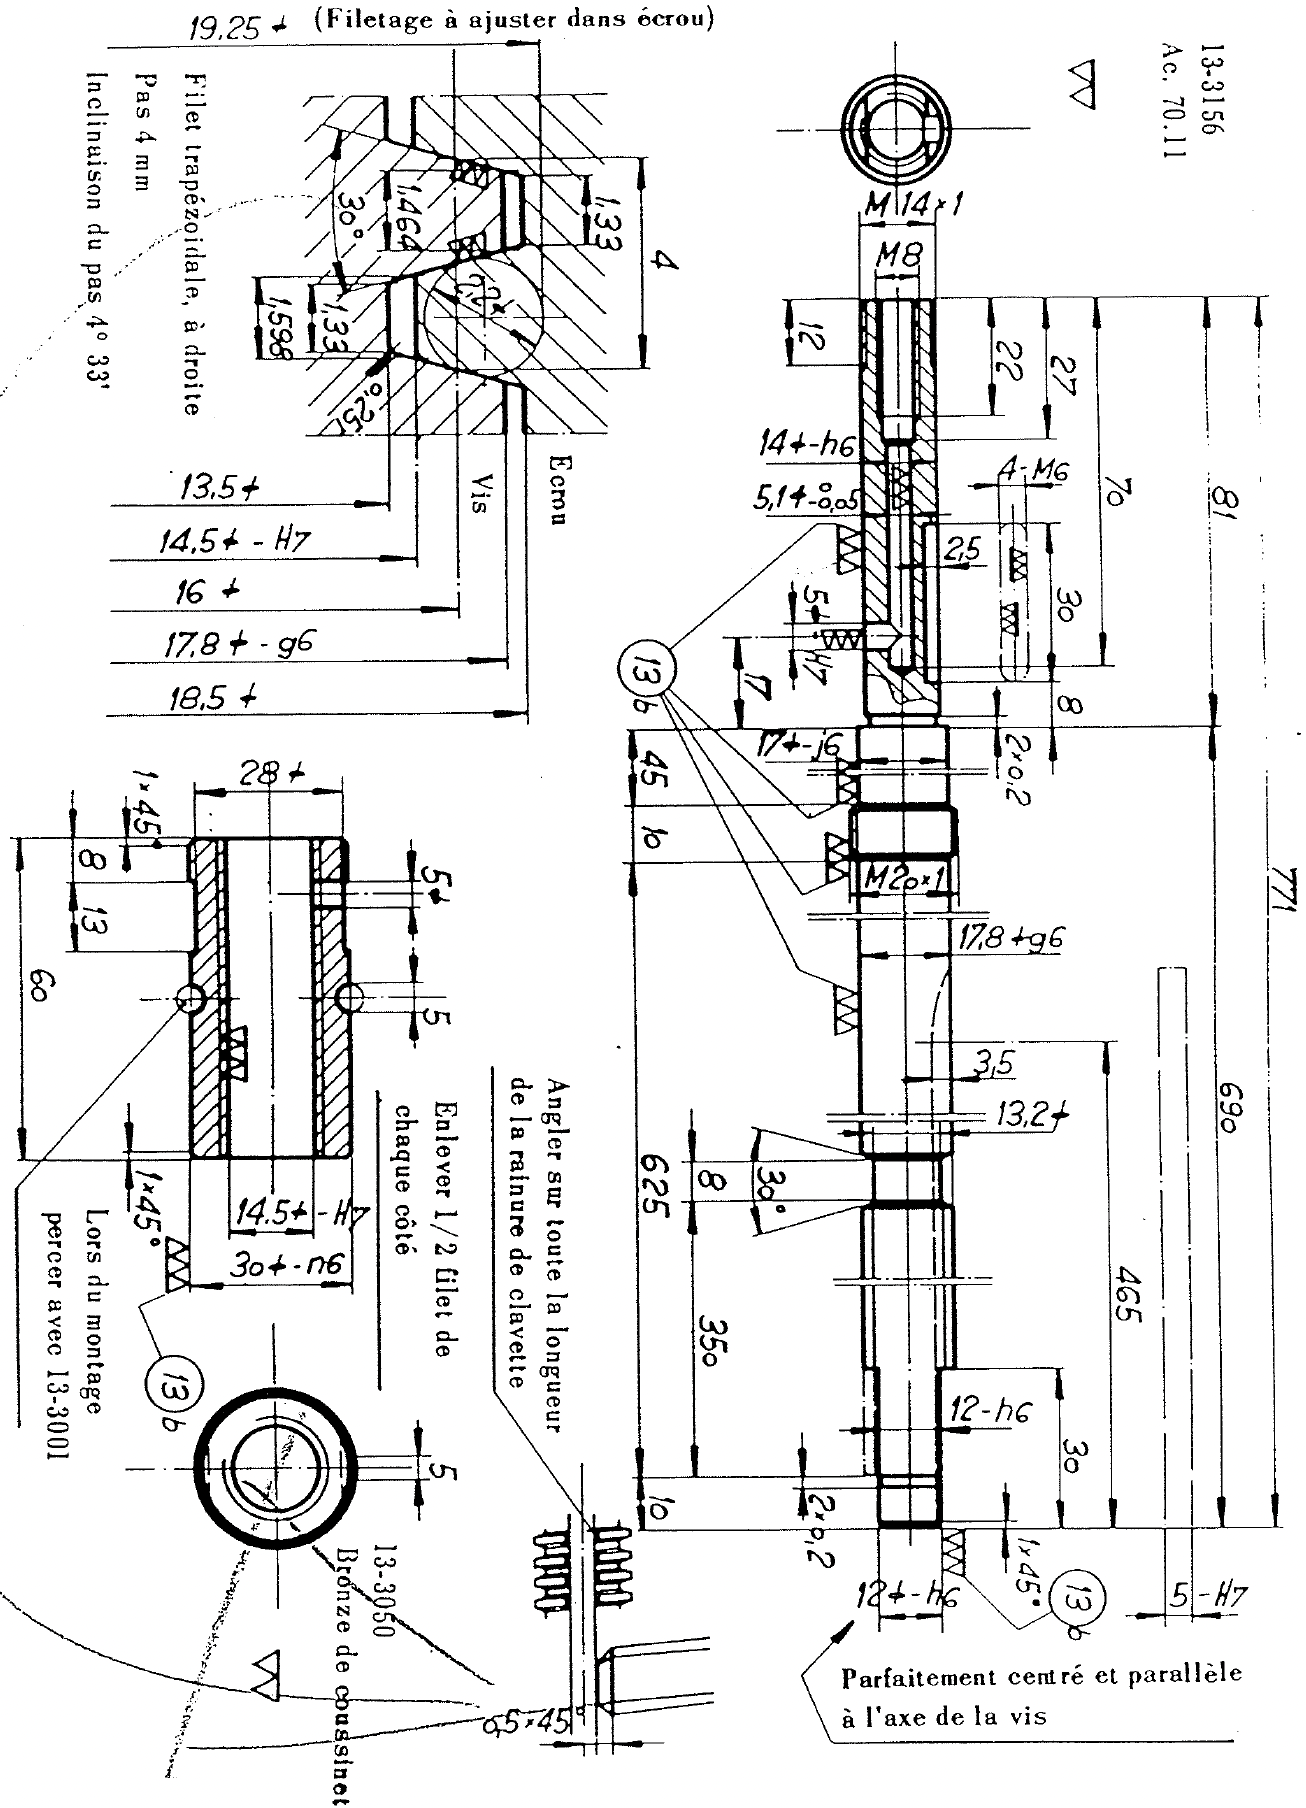
\includegraphics[width=.87\linewidth]{images/page_66}
    \label{fig:page_66}
\end{figure}
    \newcommand{\assemblyDrawing}[4][.95]{%
    \newpage
    \section{#2}
    \begin{figure}[ht]
        \centering
        \includegraphics[width=#1\linewidth]{images/assemblies/page_#3_#4}
        \label{fig:page_#3_assembly_#4}
    \end{figure}%
}

\assemblyDrawing{Transmission Housing}{68}{transmission_housing}
\assemblyDrawing{Transmission Housing}{69}{transmission_housing}
\assemblyDrawing[.85]{Variable Speed Drive}{70}{variable_speed_drive}
\assemblyDrawing{Base Frame}{71}{base_frame}
\assemblyDrawing{Longitudinal Slide}{72}{longitudinal_slide}
\assemblyDrawing{Longitudinal Slide}{73}{longitudinal_slide}
\assemblyDrawing[.75]{Rapid Feed}{74}{rapid_feed}
\assemblyDrawing{Disengagable Handwheel for Vertical Movement}{75}{disengagable_handwheel_for_vertical_movement}
\assemblyDrawing{Automatic Vertical Slide}{76}{automatic_vertical_slide}
\assemblyDrawing{Automatic Vertical Slide}{77}{automatic_vertical_slide}
\assemblyDrawing[.75]{Automatic Vertical Slide}{78}{automatic_vertical_slide}
\assemblyDrawing{Automatic Vertical Slide}{79}{automatic_vertical_slide}
\assemblyDrawing[.9]{Horizontal Spindle Carrier Head}{80}{horizontal_spindle_carrier_head}
\assemblyDrawing[.9]{Vertical Head}{81}{vertical_head}
\assemblyDrawing[.9]{Fast Head}{82}{fast_head}
\assemblyDrawing{Mortising Head}{83}{mortising_head}
\assemblyDrawing{External Piping}{84}{external_piping}
\assemblyDrawing{Counter Support}{85}{counter_support}


\section{Oil pan}
\begin{figure}[ht]
    \centering
    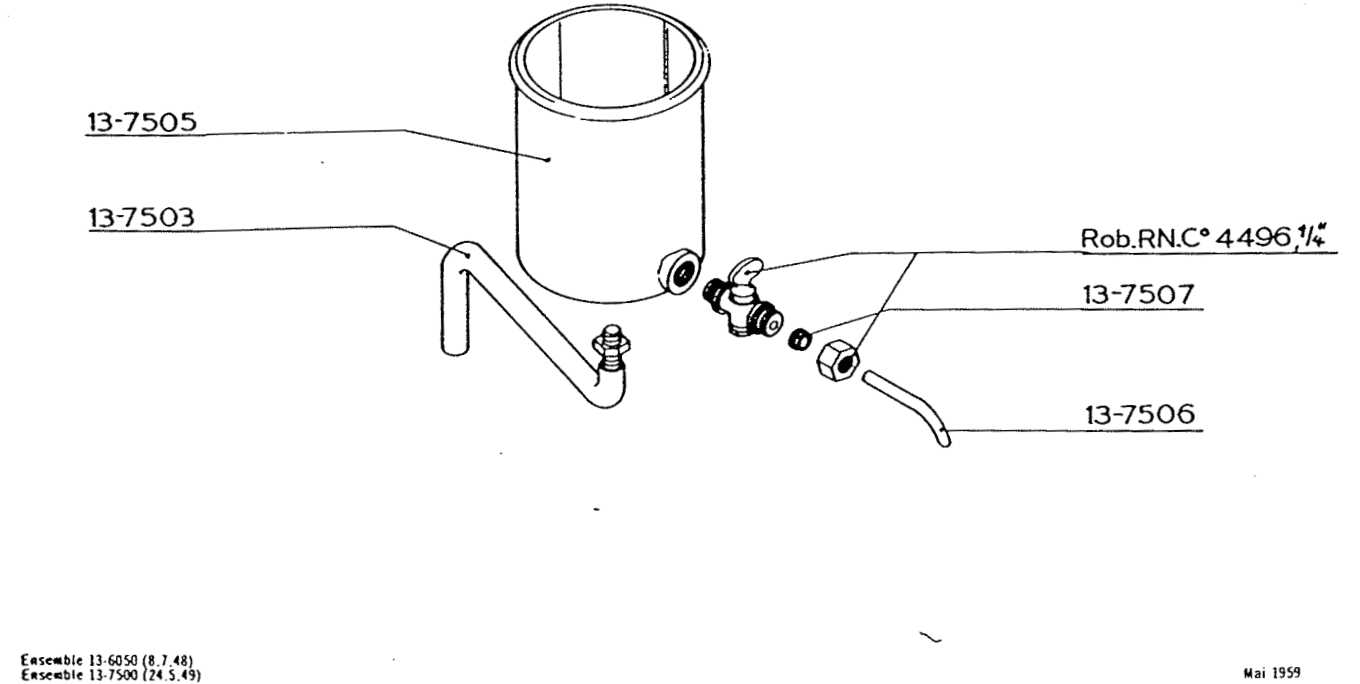
\includegraphics[width=.9\linewidth]{images/assemblies/page_85_oil_pan}
    \label{fig:page_85_assembly_oil_pan}
\end{figure}
\assemblyDrawing[.9]{Circular Plate with Vernier and 3 Disk Indexing Device}{86}{circular_plate_with_vernier_and_3_disk_indexing_device}
\cover[white]{200}{90}{8}{1}
\assemblyDrawing{Rack Controls}{87}{rack_controls}
\assemblyDrawing[.9]{Wedge Supports}{88}{wedge_supports}
\assemblyDrawing{Wedge Support}{89}{wedge_support}
\assemblyDrawing{Rotary Vises}{90}{rotary_vises}
\assemblyDrawing[.9]{Graduated Scales}{91}{graduated_scales}
\assemblyDrawing{Simple Indexer Tailstock Quick Clamp 20W}{92}{simple_indexer_tailstock_quick_clamp_20w}
\assemblyDrawing{Tailstock with Quill Tailstock}{93}{tailstock_with_quill_tailstock}

\end{document}
